
\documentclass[aspectratio=169]{beamer}


\usepackage{booktabs} % Allows the use of \toprule, \midrule and \bottomrule for better rules in tables

%%% Customize Theme %%%%%%%%%%%%%%%%%%%%%%
\usetheme{Madrid}

%%%%%%%%%%%%%%%%%%%%%%%%%%%%%%%%%%%%%%%%%%%%%%%%%%
%%%%%%%%%%%%~~~~~~~~PACKAGES~~~~~~~~~%%%%%%%%%%%%%
%%%%%%%%%%%%%%%%%%%%%%%%%%%%%%%%%%%%%%%%%%%%%%%%%%

\usepackage[utf8]{inputenc}
\usepackage[T1]{fontenc}
\usepackage[francais]{babel}
\usepackage{graphicx}
\usepackage{amsmath,amsfonts,amsthm,amssymb}
\usepackage{algorithm}
\usepackage{algorithmic}
\usepackage{fancyhdr}
%\usepackage[]{algorithm2e}
\usepackage{hyperref}
\usepackage{color}
\usepackage{pstricks}
%\usepackage{stmaryrd}
\usepackage{bbm}
\usepackage{bm}
\usepackage{showlabels}
\usepackage{cases}
\usepackage{array}
\usepackage{relsize,exscale}
\usepackage{caption}
\usepackage{times}
\usepackage{subcaption}
\usepackage{graphicx} 
\usepackage{epstopdf}
\usepackage{tikz}
\usepackage{glossaries}
\usepackage{pgfplots}
\pgfplotsset{compat=1.18}
%%%%%%%%%%%%%%%%%%%%%%%%%%%%%%%%%%%%%%%%%%%%%%%%%%%%%%%%%%%%%
%%%%%~~~~~~~~~~~~~~~MATH ENVIRONMENT~~~~~~~~~~~%%%%%%%%%%%%%%
%%%%%%%%%%%%%%%%%%%%%%%%%%%%%%%%%%%%%%%%%%%%%%%%%%%%%%%%%%%%%

\let\definition\relax
\newtheorem{definition}{Définition}
\newtheorem{proposition}{Propriété}
\newtheorem{thm}{Théorème}
\newtheorem{corollaire}{Corollaire}
\newcommand{\myabs}[1]{\left \lvert {#1} \right \rvert}

% Bottom right hand color
\setbeamercolor*{structure}{bg=myRed!20,fg=myRed!90}

\setbeamercolor*{palette primary}{use=structure,fg=white,bg=structure.fg} %?
\setbeamercolor*{palette secondary}{use=structure,fg=myRed,bg=white}
    %bottom left of footer & bar between title & top bubbles
\setbeamercolor*{palette tertiary}{use=structure,fg=white,bg=myRed} 

\setbeamercolor{frametitle}{bg=myRed!85,fg=white} %title of each slide

\setbeamercolor*{titlelike}{parent=palette primary} %?
%\setbeamercolor{titlelike}{parent=palette primary,fg=structure.fg!50!myRed}

%for miniframe (very top) AND center footer
\setbeamercolor{section in head/foot}{fg=myOrange, bg=white}

%%% Specific Colors %%%
\setbeamercolor{item projected}{bg=myOrange}
\setbeamertemplate{enumerate items}{bg=myOrange}

\setbeamercolor{itemize item}{fg=myOrange}
\setbeamercolor{itemize subitem}{fg=myOrange}

\setbeamercolor{button}{bg=myOrange}

%%% Edits ONLY the TOC slide %%%
\setbeamercolor{section in toc}{fg=black}
\setbeamercolor{subsection in toc}{fg=black}

%%%%%%%%%%%%%%%%%%%%%%%%%%%%%%%%%%%%%%%%%%%%%%%%%%%%%%%%%%%%%%%%%%
%%%%%~~~~~~~~~~~~~~RGB COLORS~~~~~~~~~~~~~~~~~~~%%%%%%%%%%%%%%%%%%
%%%%%%%%%%%%%%%%%%%%%%%%%%%%%%%%%%%%%%%%%%%%%%%%%%%%%%%%%%%%%%%%%%
\definecolor{myRed}{RGB}{120,4,4}
\definecolor{myOrange}{RGB}{227, 125, 0}
\definecolor{cadmiumgreen}{rgb}{0.0, 0.42, 0.24}
\definecolor{armygreen}{rgb}{0.29, 0.33, 0.13}
\definecolor{darkgreen}{rgb}{0.0, 0.2, 0.13}
\definecolor{officegreen}{rgb}{0.0, 0.5, 0.0}
\definecolor{blue-violet}{rgb}{0.54, 0.17, 0.89}
\definecolor{yellow-orange}{rgb}{1, 0.6, 0}
\definecolor{byzantine}{rgb}{0.74, 0.2, 0.64}
\definecolor{bulgarianrose}{rgb}{0.28, 0.02, 0.03}
\definecolor{burntorange}{rgb}{0.8, 0.33, 0.0}
\definecolor{calpolypomonagreen}{rgb}{0.12, 0.3, 0.17}
\definecolor{midnightblue}{rgb}{0.1, 0.1, 0.44}
\definecolor{darkmagenta}{rgb}{0.55, 0.0, 0.55}
\definecolor{darkmidnightblue}{rgb}{0.0, 0.2, 0.4}
\definecolor{royalblue}{rgb}{0.25, 0.41, 0.88}
\newcommand{\dps}{\displaystyle}



\setbeamercolor{block title}{bg=myOrange, fg=white}
\setbeamercolor{block body}{bg=myOrange!20}

\newcommand{\corrige}[1]{\textcolor{midnightblue}{\textbf{Correction :} #1}}

%---------------------------------------------------------
%	SELECT FONT THEME & FONTS
%---------------------------------------------------------
\usefonttheme{default} % Typeset using the default sans serif font
\usepackage{palatino} % Use the Palatino font for serif text
\usepackage[default]{opensans} % Use the Open Sans font for sans serif text
\useinnertheme{circles}
\setbeamerfont{headline}{size=\tiny}

%---------------------------------------------------------
%	SELECT OUTER THEME
%---------------------------------------------------------
% Outer themes change the overall layout of slides, such as: header and footer lines, sidebars and slide titles. Uncomment each theme in turn to see what changes it makes to your presentation.

%\useoutertheme{default}
%
\useoutertheme{miniframes}

%\useoutertheme{infolines}
%\useoutertheme{smoothbars}
%\useoutertheme{sidebar}
%\useoutertheme{split}
%\useoutertheme{shadow}
%\useoutertheme{tree}
%\useoutertheme{smoothtree}

%---------------------------------------------------------
%	PRESENTATION INFORMATION
%---------------------------------------------------------

\title[Dérivation et Intégration]{Dérivation et Intégration \\ A1 Semestre 2}
%\subtitle{}
\author[JAD DABAGHI]{JAD DABAGHI}

\institute[]{Enseignant-Chercheur en  Mathématiques DVRC \\ \smallskip \textit{jad.dabaghi@devinci.fr}}
\date[24 Avril 2024]
%\date[\today]


%\logo{\includegraphics[width=2.5cm]{Logo_ESILV.png}}

\newcommand{\sh}{\mathrm{sh}}
\newcommand{\ch}{\mathrm{ch}}


\makeatletter
\let\beamer@writeslidentry@miniframeson=\beamer@writeslidentry%
\def\beamer@writeslidentry@miniframesoff{%
  \expandafter\beamer@ifempty\expandafter{\beamer@framestartpage}{}% does not happen normally
  {%else
    % removed \addtocontents commands
    \clearpage\beamer@notesactions%
  }
}
\newcommand*{\miniframeson}{\let\beamer@writeslidentry=\beamer@writeslidentry@miniframeson}
\newcommand*{\miniframesoff}{\let\beamer@writeslidentry=\beamer@writeslidentry@miniframesoff}
\makeatother


%---------------------------------------------------------
%---------------------------------------------------------
%---------------------------------------------------------
\begin{document}




%---------------------------------------------------------
%	TITLE SLIDE
%---------------------------------------------------------
\section{}
\miniframesoff
\begin{frame}
	\titlepage % Output the title slide, automatically created using the text entered in the PRESENTATION INFORMATION block above
 \hspace{13.5 cm} 
 \includegraphics[scale = 0.3]{Logo_ESILV.png}
\end{frame}


\begin{frame}
	\frametitle{Table des matières} % Slide title, remove this command for no title
	
	\tableofcontents % Output the table of contents (all sections on one slide)
	%\tableofcontents[pausesections] % Output the table of contents (break sections up across separate slides)
\end{frame}



%%%%%%%%%%%%%%%%%%%%%%%%%%%%%%%%%%%%%%%%%%%%%%%%%%%%%%
%%%%%%%%%%%%~~~~~~~~INTRODUCTION~~~~~~~~~%%%%%%%%%%%%%
%%%%%%%%%%%%%%%%%%%%%%%%%%%%%%%%%%%%%%%%%%%%%%%%%%%%%%

\section{Introduction} 

 
%------------------------------------------------
\begin{frame}
	\frametitle{Objectifs}
            \begin{enumerate}
                \item 
Comprendre les comportements locaux et asymptotiques des fonctions
                \vspace{0.4 cm}
                \item
Savoir manipuler les développements limités
%% \vspace{0.4 cm}
%% \item
%% Connaître les principales propriétés des fractions rationnelles
\vspace{0.4 cm}
\item
  Savoir calculer plusieurs familles d'intégrales
  \vspace{0.4 cm}
\item
Introduction à l'analyse à plusieurs variables.
\end{enumerate}   
\end{frame}

\begin{frame}
    \frametitle{Contenu du module}
    \begin{enumerate}
        
   \item
            Chapitre 1 : Relations de comparaison \quad \alert{(CMO 1)}
                       \vspace{0.15 cm}
\begin{itemize}
\item
Un peu de topologie,  
       continuité d’une fonction en un point.
    \item 
    Fonctions dominées, fonctions négligeables, fonctions équivalentes.
\end{itemize}
   \vspace{0.3 cm}
\item
    Chapitre 2 : Développements limités \quad \alert{(CMO $2$)}
               \vspace{0.15 cm}

\begin{itemize}
    \item 
    Formules de Taylor, opérations sur les développements limités, applications.
    \item \textcolor{cadmiumgreen}{\textbf{Contrôle continu 1h 14 Mars 2023}}
\end{itemize}
\vspace{0.15 cm}
\item
Chapitre 3 : Calcul d'intégrales \quad \alert{(CMO 3)}
\vspace{0.15 cm}
\item
Chapitre 4 : Introduction à l'analyse à plusieurs variables \quad \alert{(CMO 4)}
\end{enumerate}            
        
\end{frame}


%%%%%%%%%%%%%%%%%%%%%%%%%%%%%%%%%%%%%%%%%%%%%%%%%%%%%%%
%%%%%%%%%%%%~~~~~~~~ANALYSE REELLE~~~~~~~~~%%%%%%%%%%%%%
%%%%%%%%%%%%%%%%%%%%%%%%%%%%%%%%%%%%%%%%%%%%%%%%%%%%%%%

\input{Analyse_reelle}

%%%%%%%%%%%%%%%%%%%%%%%%%%%%%%%%%%%%%%%%%%%%%%%%%%%%%%%%%%%%%%%%
%%%%%%%%%%%%~~~~~~~~RELATIONS COMPARAISONS~~~~~~~~~%%%%%%%%%%%%%
%%%%%%%%%%%%%%%%%%%%%%%%%%%%%%%%%%%%%%%%%%%%%%%%%%%%%%%%%%%%%%%%

\section{Relations de comparaison}

%------------------------------------------------
\begin{frame}
\frametitle{Fonctions dominées}

\begin{definition}
Soit $f : I \rightarrow \mathbb{R}$ et $\varphi : I \rightarrow \mathbb{R}$ et $a \in I$. 
 Alors $f$ est \textbf{dominée} par $\varphi$ au voisinage de $a$, s'il existe une fonction $u : I \rightarrow \mathbb{R}$ bornée au voisinage de $a$ et telle que $f = \varphi u$ au voisinage de $a$. 
 On note
 \begin{equation*}
     f = \mathcal{O}(\varphi)
 \end{equation*} 
\end{definition}
\invisible<1>{
\vspace*{0.3 cm}
\textcolor{cadmiumgreen}{\textbf{Exemple} : } 
$f(x) = x^2 \sin \left(\dps \frac{1}{x} \right)$  sur $\ \mathbb{R}$ et $\varphi(x) = x^2$.
Alors
\begin{equation*}
    f(x) = \varphi(x) \textcolor{red}{u}(x) \quad \text{avec} \quad \textcolor{red}{u}(x) = \sin \left(\frac{1}{x} \right). 
\end{equation*}
Or \alert{$u$ est bornée} donc $f = \mathcal{O}(\varphi)$.
 \invisible<2>{
 }}
\end{frame}
%%%%%
\begin{frame}
\frametitle{Fonctions négligeables}
\vspace{-0.1 cm}
\begin{definition}
on dit que $f$ est \textbf{négligeable} devant $\varphi$ au voisinage de $a$, s'il existe une fonction $\varepsilon$ définie sur $I$ tel que $f = \varphi \varepsilon$ au voisinage de $a$ et $\lim_{\substack{a}} \varepsilon = 0$. On note $f = o(\varphi)$.
  \end{definition}
  \invisible<1>{
  \textcolor{cadmiumgreen}{\textbf{Exemple :}}
  $x^3 = o(x^2)$ au voisinage de $0$ car $x^3 = \textcolor{red}{x} \times x^2$ avec $\textcolor{red}{\varepsilon}(x) = x$ et $\dps \lim_{x \rightarrow 0} \textcolor{red}{\varepsilon}(x) = 0$.
  \begin{figure}[h]
    \centering
    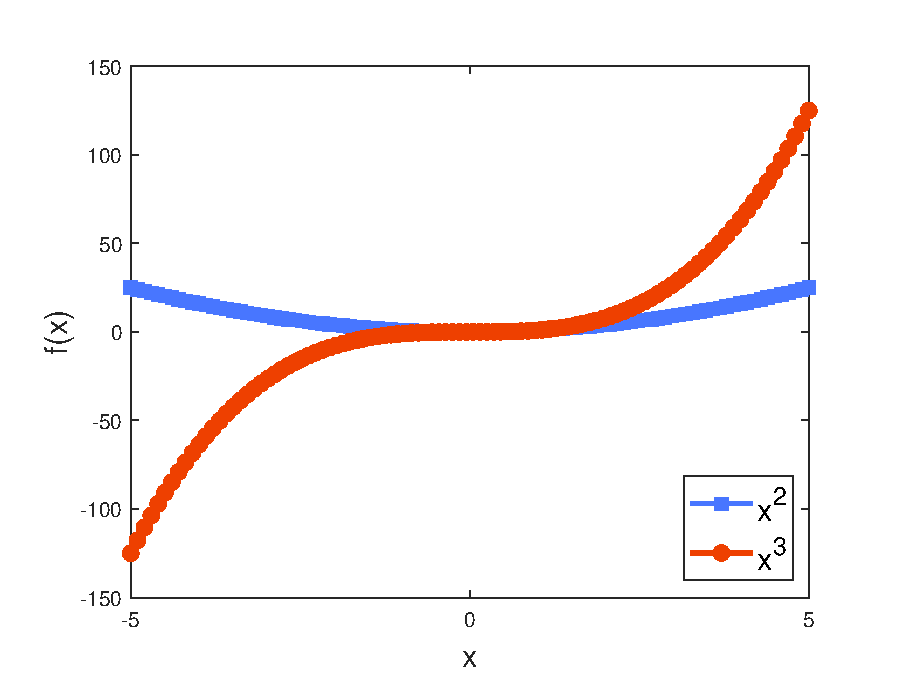
\includegraphics[scale = 0.35]{fig_x2_x3}
\quad
    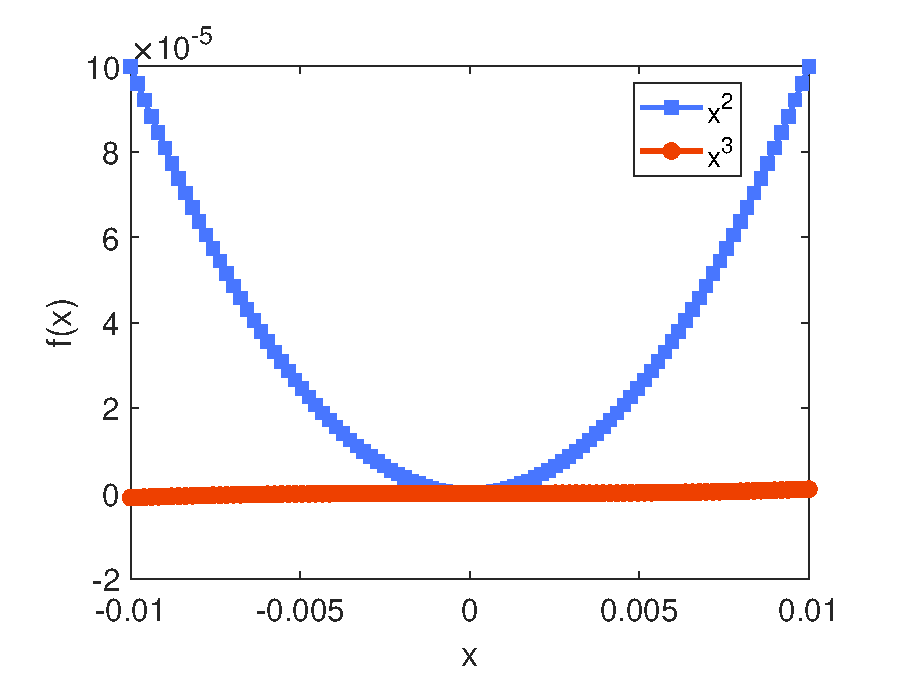
\includegraphics[scale = 0.35]{fig_x2_x3_zoom}
  \end{figure}
  \invisible<2>{
  }}
\end{frame}

%------------------------------------------------
\begin{frame}
	\frametitle{Quelques résultats}
		\begin{proposition}
Soit $f : I \rightarrow \mathbb{R}$ une fonction et $a \in I$.
\vspace{0.2 cm}
   \begin{enumerate}
   \item
     La fonction $f$ est bornée au voisinage de $a$ si, et seulement si $f = \mathcal{O}(1)$.
\vspace{0.3 cm}
   \item
     La fonction $f$ tend vers $0$ en $a$ si, et seulement si $f= o(1)$.
     \end{enumerate}
\end{proposition}
\vspace{0.2 cm}
\invisible<1>{
\textbf{Démonstration :}
\invisible<2>{
}}
\vspace{0.2 cm}
  \begin{enumerate}
  \item
 \invisible<1>{
 $\alert{(\Rightarrow)}$
On suppose $f$ bornée au voisinage de $a$. 
$\forall x \in \textcolor{cadmiumgreen}{\mathcal{V}_{a}}$, $|f(x)| = f(x) \times \underbrace{\textcolor{darkmagenta}{1}}_{\text{bornée}}$. 
    Donc $f = \mathcal{O}(1)$.
    \\
    \invisible<2>{
  \vspace{0.2 cm}
   $\alert{(\Leftarrow)}$  $f = \mathcal{O}(1)$. 
   Alors $\exists \varphi$  bornée sur $\textcolor{cadmiumgreen}{\mathcal{V}_{a}}$ tel que $f = \varphi \times 1$ sur $\textcolor{cadmiumgreen}{\mathcal{V}_{a}}$. 
Donc $f$ bornée sur $\textcolor{cadmiumgreen}{\mathcal{V}_{a}}$.
\invisible<3>{
}}}
\end{enumerate}
\end{frame}
%------------
\begin{frame}
\begin{enumerate}\setcounter{enumi}{1}
  \item
$\alert{(\Rightarrow)}$  $f$ tend vers $0$ en $a$ :
\begin{equation*}
\forall \varepsilon > 0 \ \exists \textcolor{cadmiumgreen}{\eta_1} > 0 \ \forall x \in ]a - \textcolor{cadmiumgreen}{\eta_1}, a + \textcolor{cadmiumgreen}{\eta_1}[, \ |f(x)|  \leq \varepsilon.    
\end{equation*}
On pose
\begin{equation*}
\begin{array}{ccccc}
\varphi & : & \mathcal{D}_f & \to & \mathbb{R} \\
 & & x & \mapsto & f(x) \\
\end{array}
\qquad \lim_{x \rightarrow a} \varphi(x) = 0
\end{equation*}
    Alors  
 $f = o(1)$.
\\
\vspace{0.4 cm}
\invisible<1>{
$\alert{(\Leftarrow)}$  $f=o(1)$ au voisinage de $a$. 
\vspace*{0.2 cm}
Alors  $\exists \textcolor{darkmagenta}{\varphi}$ définie au voisinage de $a$ tel que $f = \textcolor{darkmagenta}{\varphi} 1$ au voisinage de $a$ avec $\lim_{a} \varphi = 0$. 

Or $\lim_{a} \varphi \in \mathcal{V}_a$ donc $\lim_{a} f = \lim_{a} \varphi = 0$.
\invisible<2>{
}}
    \end{enumerate}
\end{frame}
%------------------------------------------------

\begin{frame}{Quelques remarques}
\begin{enumerate}
    \item <1->
Lorsque $f = o(g)$ au voisinage de $a \in I$, $f = g \times \varepsilon$ au voisinage de $a$ et $\lim_{a} \varepsilon = 0$. Mais, $\lim_{a} \varepsilon \not \rightarrow 0$ sur $I$ tout entier.
\\
\vspace{0.2 cm}
  \textcolor{cadmiumgreen}{\textbf{Contre exemple :}} 
  \begin{equation*}
      f : x \mapsto x^3 \quad \text{et} \quad g : x \mapsto x^2 \quad \text{sur} \ \mathbb{R}.
  \end{equation*}
  On a $f=o(g)$ au voisinage de $0$ (\textcolor{darkmagenta}{$\varepsilon(x) = x$}) mais $\varepsilon(x) \neq 0 \ \forall x \in \mathbb{R}^{*}$.  
\\
\vspace{0.2 cm}
 \item <2->
  Si $f=o(h)$ et $g=o(h)$ au voisinage de $a$ alors $f$ n'est pas forcément égal à $g$. 
  \\
\vspace{0.2 cm}
  \textcolor{cadmiumgreen}{\textbf{Contre exemple :}}
  \begin{equation*}
   f : x \mapsto x^3 \quad    g : x \mapsto x^4 \quad h : x \mapsto x^2.
  \end{equation*}
  On a $f=o(h)$ au voisinage de $0$ et $g=o(h)$ au voisinage de $0$ mais $f \neq g$.
\vspace{0.3 cm}
    \item <3->
  Le même phénomène s'observe pour la notation $\mathcal{O}$.
\end{enumerate}
      
\end{frame}
%%--------------------
\begin{frame}{Règles de calcul}

\begin{proposition}
    \begin{enumerate}
  \item
  $f = o(\varphi) \Rightarrow f = \mathcal{O}(\varphi) \qquad  $ \textcolor{midnightblue}{(négligeable $\Rightarrow$ bornée)}
  \vspace{0.3 cm}
  \item
$f_1 = \mathcal{O}(\varphi)$ et $f_2 = \mathcal{O}(\varphi)$ $\Rightarrow f_1 + f_2 = \mathcal{O}(\varphi)$ \quad  \textcolor{midnightblue}{\small{(somme de fonctions bornée est bornée)}}
\vspace{0.3 cm}
\item
$f_1 = \mathcal{O}(\varphi_1)$ et $f_2 = \mathcal{O}(\varphi_2)$ $\Rightarrow f_1 f_2 = \mathcal{O}(\varphi_1 \varphi_2)$ 
\vspace{0.3 cm}
\item
$f_1 = o(\varphi)$ et $f_2 = o(\varphi)$ $\Rightarrow f_1  + f_2 = o(\varphi)$ \quad \textcolor{midnightblue}{\small{(somme de termes négligeable est négligeable)}}
\vspace{0.3 cm}
\item
$f_1 = o(\varphi_1)$ et $f_2 = o(\varphi_2)$ $\Rightarrow f_1 f_2 = o(\varphi_1 \varphi_2)$
\vspace{0.3 cm}
\item
$f = \mathcal{O}(\varphi_1)$ et $\varphi_1 = \mathcal{O}(\varphi_2)$ $\Rightarrow f = \mathcal{O}(\varphi_2)$ \quad \textcolor{midnightblue}{\small{(transitivité de la domination)}}
\vspace{0.3 cm}
\item
$f = o(\varphi_1)$ et $\varphi_1 = o(\varphi_2)$ $\Rightarrow f = o(\varphi_2)$ \textcolor{midnightblue}{\small{(transitivité de la négligence)}}
  \end{enumerate}
  \end{proposition}
\end{frame}
%------------
\begin{frame}{Démonstration}
\begin{enumerate}
        \item <1-> 
    $f = o(\varphi)$ au voisinage d'un point $a$ $\Rightarrow \ f = g \varphi$ au voisinage de $a$ et \textcolor{darkmagenta}{$\lim_{a} g = 0$}. 
%Ce qui s'écrit aussi à l'aide de la définition de la limite
\begin{equation*}
\textcolor{darkmagenta}{\forall \varepsilon > 0 \ \exists \eta > 0 \ \forall x \in  ]a-\eta, a+\eta[, \ |g(x)| \leq \varepsilon.}
\end{equation*}
La fonction $g$ est donc bornée au voisinage de $a$.
Alors $f = \mathcal{O}(\varphi)$.

\item <2->
  \invisible<1>{
    $f_1 = \mathcal{O}(\varphi)$ alors $f_1 = \varphi u$ au voisinage de $a$ où $u$ est bornée au voisinage de $a$.
  \begin{equation*}
    \exists \eta_1 > 0 \ \forall x \in ]a - \eta_1, a + \eta_1[, \ f_1(x) = \varphi(x) u(x).
  \end{equation*}
  \invisible<2>{
    $f_2 = \mathcal{O}(\varphi)$ donc $f_2 = \varphi v$ au voisinage de $a$.
\begin{equation*}
 \exists \eta_2 > 0 \ \forall x \in ]a - \eta_2, a + \eta_2[, \ f_2(x) = \varphi(x) v(x).
\end{equation*}
\invisible<3>{
Pour \textcolor{darkmagenta}{$\eta = \min(\eta_1, \eta_2)$} on a $\forall x \in ]a - \textcolor{darkmagenta}{\eta}, a + \textcolor{darkmagenta}{\eta} [ \ (f_1+ f_2)(x) = \varphi(x) (u + v)(x)$. 
  Comme $u+v$ bornée au voisinage de $a$ on a $f_1 + f_2 = \mathcal{O}(\varphi)$.
  \invisible<4>{
  }}}}
\end{enumerate}
    
\end{frame}
%--------
\begin{frame}
\frametitle{Démonstration}
    \begin{enumerate}\setcounter{enumi}{3}
    \item 
      \begin{itemize}
      \item
        $f_1 = o(\varphi)$ au voisinage de $a$ alors il existe une fonction $\varepsilon_1$ définie au voisinage de $a$ tel que
        \begin{equation*}
\lim_{x \rightarrow a} \varepsilon_1(x) = 0 
        \end{equation*}
        et vérifiant $f_1 = \varepsilon_1 \varphi$ au voisinage de $a$
        \vspace*{0.3 cm}
      \item
$f_2 = o(\varphi)$ au voisinage de $a$ alors il existe une fonction $\varepsilon_2$ définie au voisinage de $a$ tel que 
\begin{equation*}
 \lim_{x \rightarrow a} \varepsilon_2(x) = 0
\end{equation*}
vérifiant $f_2 = \varepsilon_2 \varphi$ au voisinage de $a$.
%\\
        \end{itemize}
        
\vspace{0.3 cm}
Ainsi, la fonction $\varepsilon = \varepsilon_1 + \varepsilon_2$ est bien définie au voisinage de $a$ et $\lim_{x \rightarrow a} \varepsilon (x) = 0$. 
Alors, $f_1 + f_2 = o(\varphi)$.
    \end{enumerate}
\end{frame}
%-----------
\begin{frame}{Règle pratique}
      \begin{proposition}
    Soit $I$ un intervalle de $\mathbb{R}$ et $a \in I$.
Supposons que $\varphi$ ne s'annule pas sur $I \backslash{a}$.
Alors au voisinage de $a$
\vspace{0.3 cm}
\begin{enumerate}
\item $f$ est dominée par $\varphi$ si, et seulement si,  $\dps \frac{f}{\varphi}$ est bornée au voisinage de $a$.
\item
$f$ est négligeable devant $\varphi$ si, et seulement si, $\lim_{x \rightarrow a} \dps \frac{f(x)}{\varphi(x)} = 0$.
\end{enumerate}
\end{proposition}
\end{frame}
%%-----------
\begin{frame}{Fonctions équivalentes}
    \begin{definition}
Soient $f$ et $g$ définies sur un intervalle $I$. On dit que $f$ est équivalente à $g$ au voisinage de $a$, s'il existe une fonction $h$ définie sur $I$ telle que $f=gh$ au voisinage de $a$ et $\lim_{x \rightarrow a} h(x) = 1$. On note $f \underset{a}{\sim}  g$.
\end{definition}
\invisible<1>{
\textcolor{cadmiumgreen}{\textbf{Exercice :}}
Soient $f$ et $g$ deux fonctions définies sur $\mathbb{R}$ par
  $f(x) = \sin(x)$ et  $g(x) = x$. Montrer que $f$ et $g$ sont équivalentes en $0$.
  
  \invisible<2>{
  \corrige{
On a $f \underset{0}{\sim} g$. 
  En effet
\begin{equation*}
\forall x \in \mathbb{R}^{*} \quad f(x)= h(x) \times g(x) \quad \text{avec} \quad h(x) = \frac{\sin(x)}{x} \underset{0}{\rightarrow} 1.
\end{equation*}
  }
  \invisible<3>{
\textbf{Remarque :} $x \mapsto x$ est un DL à l'ordre $1$ de la fonction $x \mapsto \sin(x)$ au voisinage de $0$.
\invisible<4>{
}}}}
\end{frame}

%%-------------------
\begin{frame}{\'{E}quivalent pour les polynômes}
\vspace{-0.5 cm}
\begin{equation*}
f(x) = \sum_{k=p}^n a_k x^k \quad \text{avec} \quad a_p \neq 0 \quad \text{et} \quad a_n \neq 0.
\end{equation*}
\begin{enumerate}
\item<1->
\textbf{\'{E}tude en $0$ :} Pour $x \in \mathbb{R}$, on a
\begin{equation*}
f(x)  = a_p x^p + a_{p+1}x^{p+1} + \cdots + a_n x^n = a_p x^p \underbrace{\left(1 + \frac{a_{p+1}}{a_p} x + \cdots + \frac{a_n}{a_p} x^{n - p} \right)}_{\textcolor{royalblue}{\rightarrow 1}}
\vspace{-0.3 cm}
\end{equation*} 
Donc
\alert{$f(x) \underset{0}{\sim} a_p x^p$}.
\item<2->
\textbf{\'{E}tude en $+ \infty$ :} Pour $x \in \mathbb{R}$ on a 
\begin{equation*}
f(x) = a_n x^n \underbrace{\left( 1 + \frac{a_{n-1}}{a_n} x^{-1} + \frac{a_{n-2}}{a_n} x^{-2} + \cdots + \frac{a_p}{a_n} x^{p-n} \right)}_{\textcolor{royalblue}{\rightarrow 1}} 
\vspace{-0.5 cm}
\end{equation*}
Donc
\alert{$f(x) \underset{+ \infty}{\sim} a_n x^n$}.
\end{enumerate}
\end{frame}

%-------
\begin{frame}{Cas pratique}
\alert{\textbf{Comment montrer que deux fonctions sont équivalentes au voisinage d'un point ?}}
\begin{proposition}
Soient $f$ et $g$ deux fonctions définies sur un intervalle $I$ et $a \in I$. 
On suppose que $g$ ne s'annule pas sur $I \backslash {a}$. Alors, la fonction $f$ est équivalente à la fonction $g$ au voisinage de $a$, si et seulement si, 
\begin{equation*}
\lim_{x \rightarrow a} \frac{f(x)}{g(x)} = 1
\end{equation*}
\end{proposition}
    
\end{frame}

%------
\begin{frame}{Résultats fondamentaux}

\begin{proposition}
Soient $f$ et $g$ deux fonctions équivalentes en $a \in I$.
\vspace{0.2 cm}
\begin{enumerate}
\item
Si $g$ a une limite finie ou infinie en $a$ alors $\lim_a f = \lim_a g$.
\vspace{0.2 cm}
\item
Si $g$ est positive sur $I$ alors $f$ est positive au voisinage de $a$.
\vspace{0.2 cm}
\item
	Si $g$ ne s'annule pas sur $I$ alors $f$ ne s'annule pas au voisinage de $a$.
\end{enumerate}
\end{proposition}
\vspace{0.3 cm}
\textcolor{cadmiumgreen}{{\textbf{Obtention d'équivalents :}}}
Si $f$ est dérivable en $a \in I$ et si $f'(a) \neq 0$, alors au voisinage de $a$ :
\begin{equation*}
\boxed{f(x) - f(a) \sim f'(a)(x-a)}
\end{equation*}
\end{frame}

%%--------
\begin{frame}{Exercices}
\begin{enumerate}
\item Montrer que $e^x - 1 \sim x$ au voisinage de $0$
  \vspace*{0.3 cm}
  \\
\item Montrer que $\ln(1 + x) \sim x$ au voisinage de $0$
  \vspace*{0.3 cm}
  \\
\item Montrer que $\sin(x) \sim x$ au voisinage de $0$
\end{enumerate}
\vspace*{0.4 cm}
\textbf{\textcolor{midnightblue}{Corrigé :}}
\vspace*{0.4 cm}
\begin{enumerate}
  \item
\textcolor{cadmiumgreen}{Comme $x \mapsto e^x$ est dérivable en $0$ et que $e^0 = 1$ on a 
\begin{equation*}
    e^x - e^0  \underset{0}{\sim} e^{\prime}(0)(x-0) \Rightarrow e^x - 1 \underset{0}{\sim} x.
\end{equation*}
}
\end{enumerate}
\end{frame}
%%%
\begin{frame}
  \begin{enumerate}
  \setcounter{enumi}{1}
\item
\textcolor{cadmiumgreen}{$x \mapsto \sin(x)$ est dérivable en $0$ et et possède une dérivée non nulle
\begin{equation*}
    \sin(x) - \sin(0) \underset{0}{\sim} \sin^{\prime}(0) (x-0) \Rightarrow \sin(x) \underset{0}{\sim} x.
\end{equation*}
}
\item
\textcolor{cadmiumgreen}{$x \mapsto \ln(1 + x)$ est dérivable en $0$ et possède une dérivée non nulle 
\begin{equation*}
 \ln(1+x) - \ln(1+0) \underset{0}{\sim} \frac{1}{1+0}(x - 0) \Rightarrow \ln(1+x) \underset{0}{\sim} x.   
\end{equation*}
}
\end{enumerate}
\end{frame}
%----------------
\begin{frame}{Substitution dans un équivalent}
\vspace{-0.1 cm}
\begin{proposition}
Soient $f$ et $g$ définies sur $I$ et équivalentes en $a$.
Si $u : \Delta \rightarrow I$ et telle que $\lim_{t \rightarrow \alpha} u(t) = a$, alors $f(u(t))$ et $g(u(t))$ sont équivalentes en $\alpha$.    
\end{proposition}
\invisible<1>{
\textbf{Application :}
Déterminer les équivalents des fonctions suivantes en $0$ :
\invisible<2>{
\begin{enumerate}
\item <1->
$\dps e^{\sin t} - 1 $
\\
\invisible<3>{
\corrige{$u(t) = \sin t$, $f(x) = e^x - 1$ et  $g(x) = x$.
On a $f \underset{0}{\sim} g$
 et $\dps \lim_{t \rightarrow 0} u(t)= 0$ donc $f(u(t)) \underset{0}{\sim} g(u(t))$.
 Finalement, $\dps e^{\sin t} - 1 \underset{0}{\sim} \sin t$.
} 
 %\item
% $ (1 + x)^{\alpha} - 1 $
% \\
% \corrige{
% $(1 + x)^{\alpha} - 1  =e^{\alpha \ln(1 + x)} - 1$.
% Soit $f(y) = e^{y} - 1$,  $g(y) = y$ et $u(x) = \alpha \ln(1 + x)$.
% \\
% On a $\dps \lim_{x \rightarrow 0} u(x) = 0$ et $f \underset{0}{\sim} g$. 
% Alors, $\dps f(u(x)) \underset{0}{\sim} g(u(x)) \ \Rightarrow (1 + x)^{\alpha} - 1 \underset{0}{\sim} \alpha \ln(1 + x)$.
% }
\item<2->
	$\ln(\cos(t))$
	\\
\invisible<4>{
 \corrige{
	On a $\ln (\cos(t)) = \ln(1 + \cos(t) - 1)$.
	Posons $u(t) = \cos(t) - 1$. Alors, $\lim_{t \rightarrow 0} u(t) = 0$.
	De plus, $\ln(1 + y) \underset{0}{\sim}y$. Donc,
	$\ln(1 + u(t)) \underset{0}{\sim} u(t)$.
	Ainsi, $\ln(\cos(t)) \underset{0}{\sim} \cos(t) - 1$.
}	
\end{enumerate}
\invisible<5>{

}}}}}
\end{frame}
%--------------
\begin{frame}{Opération sur les fonctions équivalentes}
\vspace*{-0.1 cm}
    \begin{proposition}
Si au voisinage de $a$ on a 
\begin{enumerate}
\item $f_1 \sim g_1$ et $g_1 \sim g_2$ alors $f_1 \sim g_2$ en $a$ \alert{(transitivité)}.
\item Si $f_1 \sim g_1$ et $f_2 \sim g_2$ alors $f_1 f_2 \sim g_1 g_2$ en $a$ \alert{(produit)}.
\item
Si $f_1 \sim g_1$ et $f_2 \sim g_2$ et si aucune de ces fonctions ne s'annule sur $I \backslash{a}$ alors $\dps \frac{f_1}{f_2} \underset{a}{\sim} \frac{g_1}{g_2}$.
\end{enumerate}
\end{proposition}

\begin{proposition}
\begin{enumerate}
    \item 
Si $g = o(f)$ au voisinage d'un point $a \in I$, alors $f+g \underset{a}{\sim} f$.
    \item
     Soient $f$ et $g$ deux fonctions définies sur un intervalle $I$ et $a \in I$.
Si $f \underset{a}{\sim} g$ alors $f = \mathcal{O}(g)$ au voisinage de $a$.
\end{enumerate}
\end{proposition}

\end{frame}
%-----------
\begin{frame}{Application}
  Déterminer un équivalent de $f$ au voisinage de $+ \infty$  définie sur $\mathbb{R}_{+}^{*}$ par $\dps f(x) = e^{\dps \frac{1}{x^2}} - e^{\dps \frac{1}{(x + 1)^2}}.$
\\
\vspace*{0.2 cm}
\invisible<1>{
\corrige{
On a 
$\forall x \in \mathbb{R}_{+}^{*}, \ 
f(x) = e^{\dps \frac{1}{x^2}} \left(\dps 1 - e^{\dps \frac{1}{(x + 1)^2}- \frac{1}{x^2}} \right) = e^{\dps \frac{1}{x^2}} \left(\dps 1 - e^{\dps \frac{-2x - 1}{x^2(x + 1)^2}} \right).$
\\
Or $1 - e^{y} \underset{0}{\sim} y$ et $\dps \lim_{ x \rightarrow + \infty} \dps \frac{-2x - 1}{x^2(x+1)^2} = 0$. 
Donc, 
$\dps 1 - e^{\dps \frac{-2x - 1}{x^2 \left( x + 1 \right)^2}} \underset{+ \infty}{\sim} \frac{-2x - 1}{x^2 \left( x + 1 \right)^2} \underset{+ \infty}{\sim} \frac{-2}{x^3}$.
De plus,
$e^{\dps \frac{1}{x^2}} \underset{+\infty}{\sim} 1$.
Ainsi,
$\dps f(x) \underset{+\infty}{\sim} -\frac{2}{x^3}$.
}
\invisible<2>{}
}
\end{frame}
%--------
\begin{frame}{Application}
    Déterminer un équivalent en $0$ de $\ln(\sin(x))$
    \\
    \vspace*{0.3 cm}
\corrige{
\invisible<1>{
On a 
\begin{equation*}
\ln(\sin(x)) = \ln \left(x \frac{\sin(x)}{x} \right) = \ln(x) + \ln \left( \frac{\sin(x)}{x} \right).
\end{equation*}
\invisible<2>{
Or 
\begin{equation*}
\dps \ln \left( \frac{\sin(x)}{x} \right) = o(\ln(x)) \quad \text{car} \quad \dps \lim_{x \rightarrow 0} \left( \frac{1}{\ln(x)} \ln \left( \frac{\sin(x)}{x} \right) \right) = 0.
\end{equation*}
\invisible<3>{
Donc
\begin{equation*}
    \dps \ln \left( \frac{\sin(x)}{x} \right) + \ln(x) \underset{0}{\sim} \ln(x).
\end{equation*}
\invisible<4>{
Ainsi
\begin{equation*}
ln(\sin(x)) \underset{0}{\sim} \ln(x).
\end{equation*}
\invisible<5>{
}}}}}
}
\end{frame}

\begin{frame}{Remarques importantes}
    \begin{enumerate}
\item<1->
\textcolor{cadmiumgreen}{\textbf{Composition d'équivalents :}}
    Si $f \sim g$ on ne peut rien dire à priori de $u \circ f$ et $u \circ g$.
    \\
\textcolor{midnightblue}{\textbf{Exemple :}} Soient $f : \mathbb{R} \rightarrow \mathbb{R}$ et $g : \mathbb{R} \rightarrow \mathbb{R}$ définies par 
\begin{equation*}
    f(x) = x \quad \text{et} \quad g(x) = x + \sqrt{x} \Rightarrow \textcolor{darkmagenta}{f(x) \underset{+ \infty}{\sim} g(x) \quad \text{mais} \quad \dps e^{f(x)} = o(e^{g(x)})}
\end{equation*} 
\item<2->
\textcolor{cadmiumgreen}{\textbf{Somme d'équivalents :}} Si $u_1 \sim u_2$ et $v_1 \sim v_2$ alors $u_1 + v_2 \not \sim u_2 + v_2$.
  \\
\textcolor{midnightblue}{\textbf{Exemple :}} 
\begin{equation*}
u(x) = \sin(2x) + \cos(x) - 1.
\end{equation*}
\vspace*{-0.2 cm}
On a 
\begin{equation*}
\sin(y) \underset{0}{\sim} y \quad \text{et} \quad \lim_{x \rightarrow 0} 2x = 0 \ \Rightarrow \ \textcolor{darkmagenta}{\sin(2x) \underset{0}{\sim} 2x} \quad \textcolor{darkmagenta}{\cos(x) - 1} = -2 \sin^2 \left(\frac{x}{2}\right)\textcolor{darkmagenta}{\underset{0}{\sim} - \frac{x^2}{2}}
\end{equation*}
Or 
\begin{equation*}
\lim_{x \rightarrow 0} \frac{u(x)}{2x} =  \left( \frac{\sin(2x)}{2x} + \frac{\cos(x) - 1}{2x} \right) = 1 \ \Rightarrow \alert{u(x) \underset{0}{\sim} 2x}
\end{equation*}
    \end{enumerate}
\end{frame}


%%%%%%%%%%%%%%%%%%%%%%%%%%%%%%%%%%%%%%%%%%%%%%%%%%%%%%%%%%%%%%%%
%%%%%%%%%%%%~~~~~~~~TAYLOR ET DL~~~~~~~~~%%%%%%%%%%%%%%%%%%%%%%%
%%%%%%%%%%%%%%%%%%%%%%%%%%%%%%%%%%%%%%%%%%%%%%%%%%%%%%%%%%%%%%%%


\miniframesoff


\begin{frame}
    \begin{center}
        \Huge{Dérivation}
    \end{center}
\end{frame}

%------------------------------------------------
\section{Dérivation}



\begin{frame}
\begin{definition}
On dit que $f$ est dérivable en $a$ si la fonction $\mathcal{T}$, appelée taux
d’accroissement de $f$ en $a$, définie sur $I\setminus\{a\}$ par
\[
\mathcal{T}(x)=\frac{f(x)-f(a)}{x-a}
\]
possède une limite finie en $a$.
Cette limite s’appelle le nombre dérivé de $f$ en $a$ et se note $f'(a)$.
\end{definition}


\textcolor{cadmiumgreen}{\textbf{Exemples : }}
\begin{enumerate}
\item Si $(\alpha,\beta)\in\mathbb{R}^2$, la fonction
$f:x\mapsto \alpha x+\beta$ est dérivable en tout point $a\in\mathbb{R}$ et
\[
\lim_{x\to a}\frac{f(x)-f(a)}{x-a}=\alpha.
\]

\item La fonction $f:x\mapsto |x|$ n’est pas dérivable en $0$ car
$\lim_{x\to 0}\frac{|x|-0}{x}= \underset{-}{+} 1 $,
la limite n'est pas unique!
\end{enumerate}
\end{frame}
%%%%%
\begin{frame}
\begin{proposition}
Si $f$ est dérivable en $a$, alors $f$ est continue en $a$.
\end{proposition}
\textbf{Démonstration :}
\begin{enumerate}
\invisible<1>{
\item $f$ est dérivable au point $a$ alors 
$f'(a)=\lim_{x\to a}\frac{f(x)-f(a)}{x-a}$.
\invisible<2>{
\item
\textcolor{midnightblue}{\textbf{Ecriture équivalente :}} $
\forall \varepsilon>0\ \exists \eta>0\ \forall x\in]a-\eta,a+\eta[ ,
\left|
\frac{f(x)-f(a)}{x-a}-f'(a)
\right|<\varepsilon$ donc
$
|f(x)-f(a)|<|x-a|(\varepsilon+|f'(a)|)<\eta(\varepsilon+|f'(a)|)$
\invisible<3>{
\item
Mq $f$ est $\mathcal{C}^0$. Soit $\varepsilon_1>0$. Mq $\exists \eta_1>0$ tq
 $|x-a|<\eta_1 \Rightarrow |f(x)-f(a)|<\varepsilon_1$.
\item
Choix de $\eta_1$ en fonction de $\varepsilon_1$ satisfaisant la Def de Continuité
\[
\varepsilon=\varepsilon_1
\quad \text{et} \quad
\eta_1=\frac{1}{2}\frac{\varepsilon_1}{\varepsilon_1+|f'(a)|}
\]
\invisible<4>{
\item
 Conclusion :
\[
|f(x)-f(a)|<|x-a|
\left(\varepsilon_1+|f'(a)|\right)
<\eta_1
\left(\varepsilon_1+|f'(a)|\right)
<\varepsilon_1.
\]
\invisible<5>{
}}}}}
\end{enumerate}



\end{frame}
%%%%
\begin{frame}
\begin{definition}
Lorsque la fonction $f$ est dérivable en tout point de $I$ on dit que $f$ est dérivable sur $I$ et la
fonction définie sur $I$ par $x\mapsto f'(x)$ est appelée fonction dérivée de $f$, et se note $f'$.
\end{definition}
\begin{proposition}
Si $f$ est dérivable sur $I$, alors elle est continue sur $I$.
\end{proposition}
\end{frame}
%%%%%%%%
\begin{frame}{Interprétations des dérivées}
\begin{enumerate}
\item
Soit une fonction $f$ définie sur $I$, pour $x\in I\setminus\{a\}$, la droite joignant les points
$A=(a,f(a))$ et $M=(x,f(x))$ a pour pente
$T_a(x)=\frac{f(x)-f(a)}{x-a}$.

Si $f$ est dérivable en $a\in I$, cette pente a pour limite $f'(a)$ quand $x$ tend vers $a$.
Le vecteur de composantes $(1,T_a(x))$ est un vecteur directeur de la corde $(AM)$, et il
tend vers $(1,f'(a))$. La droite passant par $A$ et de pente $f'(a)$ est donc la tangente
à la courbe d’équation $y=f(x)$.
\vspace*{0.3 cm}
\item
La tangente en $A$ est horizontale si et seulement si $f'(a)=0$.
\vspace*{0.3 cm}
\item
Lorsque $f(t)$ est l’abscisse à l’instant $t$ d’un point en mouvement rectiligne, pour
$t\neq a$ le taux d’accroissement
$T_a(t)=\frac{f(t)-f(a)}{t-a}$
représente la vitesse moyenne entre les instants $a$ et $t$, et sa limite $f'(a)$ représente
la vitesse instantanée à l’instant $a$.
\end{enumerate} 

\end{frame}

%%%%%%
\begin{frame}
\frametitle{Opérations sur les dérivées}
\begin{proposition}
Soient $f$ et $g$ deux fonctions définies sur $I$ et $(\lambda, \mu) \in \mathbb{R}^2$. 
Si $f$ et $g$ sont dérivables en $a$ alors
les fonctions $\lambda f + \mu g$  sont dérivables en $a$ et :
\begin{equation}
(\lambda f + \mu g)^{\prime}(a) = \lambda f(a) + \mu g(a) \quad \text{and} \quad (f g)^{\prime}(a)= f^{\prime}(a) g(a) + f(a) g^{\prime}(a)
\end{equation}
\end{proposition}
\textbf{Démonstration :}
\begin{enumerate}
\item
\begin{equation}
\begin{split}
(fg)'(a)
&= \lim_{x \to a} \frac{(fg)(x) - (fg)(a)}{x - a} \\
&= \lim_{x \to a} \frac{(fg)(x) - (fg)(a) + f(x)g(a) - f(x)g(a)}{x - a} \\
&= \lim_{x \to a} \frac{g(a)\bigl(f(x) - f(a)\bigr) + f(x)\bigl(g(x) - g(a)\bigr)}{x - a} \\
&= f'(a)g(a) + f(a)g'(a).
\end{split}
\end{equation}
\end{enumerate}
\end{frame}
%%%%%%%
\begin{frame}
\begin{enumerate}
\setcounter{enumi}{1}
\item
\begin{equation}
\begin{split}
(\lambda f + \mu g)^{\prime}(a)
&= \lim_{x \to a} \frac{(\lambda f + \mu g)(x) - (\lambda f + \mu g)(a)}{x - a} \\
&= \lambda \underbrace{\lim_{x \to a} \frac{f(x) - f(a)}{x - a}}_{f^{\prime}(a)}
+ \mu \underbrace{\lim_{x \to a} \frac{g(x) - g(a)}{x - a}}_{g^{\prime}(a)}
\end{split}
\end{equation}
\end{enumerate}
\begin{corollaire}
Si $f$ et $g$ sont deux fonctions dérivables sur $I$, alors la fonction $fg$ est dérivable sur $I$ et
\begin{equation}
\begin{split}
(f+g)^{\prime} &= f^{\prime} + g^{\prime}
\\
(fg)^{\prime} &= fg^{\prime} + f^{\prime}g
\end{split}
\end{equation}
\end{corollaire}
\end{frame}
%%%%%%
\begin{frame}
\frametitle{Inverse et quotient}
\vspace*{-0.15 cm}
\begin{proposition}
Soit $f$ une fonction dérivable en $a$ et ne s'annulant pas sur $I$ alors $\frac{1}{f}$ est dérivable en $a$ et
\vspace*{-0.2 cm}
\begin{equation*}
\left(\frac{1}{f}\right)^{\prime}(a) = - \frac{f^{\prime}(a)}{\left(f(a)  \right)^2}
\end{equation*}
\end{proposition}
\vspace*{-0.1 cm}
\textbf{Démonstration :} Soit $x \in I$ et $a \in I$ tel que $x \neq a$.
\begin{equation*}
\lim_{x \to a} \frac{\dfrac{1}{f(x)} - \dfrac{1}{f(a)}}{x - a}
= \lim_{x \to a} \left( - \frac{1}{f(x)f(a)} \right)
\frac{f(x) - f(a)}{x - a} 
= - \frac{f^{\prime}(a)}{(f(a))^{2}}.
\end{equation*}
\vspace*{-0.2 cm}
\begin{corollaire}
Soient $f$ et $g$ deux fonctions dérivables en $a$. 
Si $g$ ne s’annule pas sur $I$ alors la fonction $\frac{f}{g}$ 
est dérivable en $a$ et
\begin{equation*}
\left(\frac{f}{g}\right)^{\prime}(a) = \frac{f^{\prime}(a) g(a) - g^{\prime}(a) f(a)}{g(a)^2}
\end{equation*}
\end{corollaire}
\end{frame}
%%%%
\begin{frame}
\frametitle{Composée et fonction réciproque}
\begin{proposition}
Soient $I$ et $J$ deux intervalles, $f$ une application de $I$ dans $J$ et $g$ une application définie sur
$J$. 
Si $f$ est dérivable en $a \in I$  et $g$ dérivable en $b = f(a)$  alors $g \circ f$ est dérivable en $a$ et
\begin{equation}
(g \circ f)^{\prime}(a) = g^{\prime}(f(a)) f^{\prime}(a)
\end{equation}
\end{proposition}
\textbf{Démonstration :} Soit $x \in I \setminus \{a\}$. On a
\begin{equation}
\begin{split}
\lim_{x \to a} \frac{(g \circ f)(x) - (g \circ f)(a)}{x - a}
&= \lim_{x \to a} \frac{g(f(x)) - g(f(a))}{x - a} \\
&= \lim_{x \to a}
\frac{g(f(x)) - g(f(a))}{f(x) - f(a)}
\frac{f(x) - f(a)}{x - a} \\
&= g'\bigl(f(a)\bigr) f'(a).
\end{split}
\end{equation}
\end{frame}
%%%%%%%%%%%%%
\begin{frame}
\textbf{\textcolor{cadmiumgreen}{Exemple :}} 
Soit $f$ la fonction définie sur $\mathbb{R}$ par
\begin{equation*}
f(x) = x^{2}\sin\!\left(\frac{1}{x}\right) \quad \text{si } x \neq 0
\quad \text{et} \quad f(0) = 0.
\end{equation*}
Montrer que $f$ est dérivable en $0$.
\\
\vspace*{0.2 cm}
\invisible<1>{
\textcolor{midnightblue}{\textbf{Correction :} Sur $\mathbb{R}^*$, $f$ est dérivable en tant que produit et composée
de fonctions dérivables. Étudions la dérivabilité de $f$ en $0$. On a
\begin{equation*}
\begin{split}
\lim_{x \to 0} \frac{f(x) - f(0)}{x - 0}
&= \lim_{x \to 0} x \sin\!\left(\frac{1}{x}\right).
\end{split}
\end{equation*}
\invisible<2>{
Or
\begin{equation*}
\left|\sin\!\left(\frac{1}{x}\right)\right| \leq 1
\quad \forall x \in \mathbb{R}.
\end{equation*}
\invisible<3>{
Donc
\begin{equation*}
\lim_{x \to 0}
\left| \frac{f(x) - f(0)}{x - 0} \right|
\leq
\lim_{x \to 0} |x|
= 0 \quad \text{$f$ est dérivable en $0$ et $f^{\prime}(0) = 0$.}
\end{equation*}
\invisible<4>{
}}}}
}
\end{frame}
%%
\begin{frame}
\begin{proposition}
Soit $f$ une application continue et strictement monotone de l’intervalle $I$ sur l’intervalle
$J = f(I)$, dérivable en $a \in I$. La fonction $f^{-1}$ est dérivable en $b = f(a)$ si, et seulement si,
$f^{\prime}(a) \neq 0$ et l’on a alors
\begin{equation*}
(f^{-1})^{\prime}(b) = \frac{1}{f^{\prime}(f^{-1}(b))}
\end{equation*}
\end{proposition}
\end{frame}
%%%%%%%%
\begin{frame}
\begin{proposition}
Soient $f$ une fonction définie sur un intervalle $I$ et $a$ un point de $I$ qui n'en est pas une borne.
Si la fonction $f$ présente un extremum local en $a$ et si elle est dérivable en $a$ alors
$f'(a)=0$.
\end{proposition}
\invisible<1>{
\textbf{Démonstration :} Par hypothèse, $f$ possède un extremum local en $a$.
Supposons que l’extremum est un minimum. 
Alors, $\exists h>0$ tel que
$\forall x \in [a-h,a+h],\ f(x)\geq f(a)$.
D’autre part, $f$ est dérivable en $a$ donc
\begin{equation*}
\lim_{x \to a} \frac{f(x)-f(a)}{x-a} = f'(a).
\end{equation*}
Si $x \in [a,a+h]$ alors $f'(a)\geq 0$.
D’autre part, si $x \in [a-h,a]$, il vient que $f'(a)\leq 0$.
En conclusion $f'(a)=0$.
\invisible<2>{
}}
\end{frame}
%%%%%%
\begin{frame}
\frametitle{Quelques remarques}
\begin{enumerate}
\item
\invisible<1>{
Une fonction peut avoir un extremum local en $a$ et ne pas être dérivable en a,
comme le prouve l’exemple de la fonction $x \mapsto |x|$ en $0$.
\invisible<2>{
\item
Si $a$ est une extrémité de l’intervalle, une fonction peut présenter un extremum
local en $a$ et être dérivable en $a$ sans que sa dérivée y soit nulle, comme le
prouve l’exemple de la restriction à $[0, 1]$ de la fonction $x \mapsto x$ qui présente un
minimum en $0$ et un maximum en $1$.
\invisible<3>{
\item
L’annulation de la dérivée de $f$ en $a$ n’est qu’une condition nécessaire pour que $f$
possède un extremum local en $a$, comme le prouve l’exemple de la fonction
strictement croissante $x \mapsto x^3$ dont la dérivée s’annule en $0$ mais qui ne possède pas d’extremum en $0$
\invisible<4>{
}}}}
\end{enumerate}
 
\end{frame}
%%%%
\begin{frame}
\frametitle{Théorème de Rolle}
\vspace{-0.2 cm}
\begin{thm}
Soit $(a,b)\in \mathbb{R}^2$ tel que $a<b$.
Soit $f$ une fonction continue sur $[a,b]$ et dérivable sur $]a,b[$
et vérifiant $f(a)=f(b)$.
Alors $\exists c\in ]a,b[$ tel que $f'(c)=0$.
\end{thm}
\begin{columns}

% ----- Colonne gauche : image -----
\begin{column}{0.55\textwidth}
\begin{tikzpicture}
\begin{axis}[
    xlabel={$x$},
    ylabel={$y$},
    xlabel style={font=\scriptsize},
    ylabel style={font=\scriptsize},
    tick label style={font=\scriptsize}, % graduations
    legend style={font=\scriptsize},     % légende
    domain=0:6.3,
    samples=120,
    xmin=0, xmax=6.3,
    ymin=-1.2, ymax=1.2,
    axis lines=box,
    legend pos=north west,
    width=\textwidth,
    height=6cm,
]
\addplot+[blue, mark=*] {cos(deg(x))};
\addlegendentry{$y=\cos(x)$}

\addplot+[red, mark=*] {-1};
\addlegendentry{$y=-1$}
\end{axis}
\end{tikzpicture}
\end{column}

% ----- Colonne droite : texte -----
\begin{column}{0.45\textwidth}
Le théorème de Rolle nous dit que le graphe de la fonction $f$
possède au moins une tangente horizontale !
\end{column}

\end{columns}
\end{frame}
%%%%%
\begin{frame}
\textbf{Démonstration :}

\begin{enumerate}
\vspace{0.3 cm}
\invisible<1>{
\item La fonction $f$ est continue sur $[a,b]$. L’image par $f$ du segment
$[a,b]$ est un segment $[m,M]$ avec $m \leq M$.
\vspace{0.3 cm}
\invisible<2>{
\item Si la fonction $f$ est constante sur $[a,b]$ il vient que $m = M$ et donc
$f' = 0$ sur $[a,b]$.
\invisible<3>{
\vspace{0.3 cm}
\item Si $m < M$, l’un des réels $m$ ou $M$ est différent de la valeur commune
prise par $f$ en $a$ et en $b$. Supposons par exemple que $m \neq f(a)$.
La fonction $f$ atteint alors la valeur $m$ en un point $c$ différent de
$a$ et $b$. Elle admet donc un minimum en ce point de l’intervalle ouvert
$]a,b[$ ce qui implique $f'(c) = 0$.
\invisible<4>{
}}}}
\end{enumerate}
\end{frame}
%%%%%
\begin{frame}
\frametitle{Interprétation cinématique}
\textit{Le théorème de Rolle nous dit qu’un point mobile sur un axe qui revient
à son point de départ a vu sa vitesse s’annuler à un instant donné.}

\begin{center}
\begin{tikzpicture}[scale=1]

\def\xleft{0}
\def\xright{8}

% ---------- t = 10 ----------
\draw[thick, blue] (\xleft,4) -- (\xright,4);
\fill[blue] (\xleft,4) circle (2pt);
\fill[blue] (\xright,4) circle (2pt);
\node at (0,4.4) {\includegraphics[width=1.6cm]{voiture.png}};
\fill[black] (0,4) circle (3pt);
\node[below] at (1.5,4) {$x(10)$};
\node[right] at (8.5,4) {$t=10$};

% ---------- t = 12 ----------
\draw[thick, blue] (\xleft,3) -- (\xright,3);
\fill[blue] (\xleft,3) circle (2pt);
\fill[blue] (\xright,3) circle (2pt);
\node at (4,3.4) {\includegraphics[width=1.6cm]{voiture.png}};
\fill[black] (4,3) circle (3pt);
\node[below] at (4,3) {$x(12)$};
\node[right] at (8.5,3) {$t=12$};

% ---------- t = 15 ----------
\draw[thick, blue] (\xleft,2) -- (\xright,2);
\fill[blue] (\xleft,2) circle (2pt);
\fill[blue] (\xright,2) circle (2pt);
\node at (7.8,2.4) {\includegraphics[width=1.6cm]{voiture.png}};
\fill[black] (8,2) circle (3pt);
\node[below] at (8,2) {$x(15)$};
\node[right] at (8.5,2) {$t=15$};

% ---------- t = 18 ----------
\draw[thick, blue] (\xleft,1) -- (\xright,1);
\fill[blue] (\xleft,1) circle (2pt);
\fill[blue] (\xright,1) circle (2pt);
\node at (3.5,1.4) {\includegraphics[width=1.6cm]{voiture.png}};
\fill[black] (3.5,1) circle (3pt);
\node[below] at (3.5,1) {$x(18)$};
\node[right] at (8.5,1) {$t=18$};

% ---------- t = 20 ----------
\draw[thick, blue] (\xleft,0) -- (\xright,0);
\fill[blue] (\xleft,0) circle (2pt);
\fill[blue] (\xright,0) circle (2pt);
\node at (0,0.4) {\includegraphics[width=1.6cm]{voiture.png}};
\fill[black] (0,0) circle (3pt);
\node[below] at (0,0) {$x(20)$};
\node[right] at (8.5,0) {$t=20$};

\end{tikzpicture}
\end{center}

\end{frame}
%%%%
\begin{frame}
\frametitle{\'{E}galité des accroissements finis}
\begin{thm}
Étant donnés des réels $a$ et $b$ tels que $a<b$ ainsi qu’une fonction $f$
continue sur $[a,b]$, dérivable sur $]a,b[$, il existe un réel $c$
appartenant à $]a,b[$ tel que
\[
f(b)-f(a) = (b-a)f'(c).
\]
\end{thm}

\textbf{Démonstration :}

\begin{enumerate}
\item Soit $k \in \mathbb{R}$ et soit $\varphi$ définie sur $[a,b]$ par $\varphi(x) = f(x) - k(x-a)$.

\item Pour $k = \dfrac{f(b)-f(a)}{b-a}$ on obtient $\varphi(a)=\varphi(b)$.

\item De plus, $\varphi \in C^0([a,b])$, dérivable sur $]a,b[$ et vérifie
$\varphi(a)=\varphi(b)$. D’après le théorème de Rolle,
\vspace*{-0.2 cm}
\begin{equation*}
\exists c \in ]a,b[ \quad \varphi'(c)=0
\iff f'(c)-k=0
\iff f'(c)=\dfrac{f(b)-f(a)}{b-a}.
\end{equation*}
\end{enumerate}

\end{frame}
%%%%%%
\begin{frame}
\frametitle{Quelques remarques}
\begin{minipage}[c]{0.49 \textwidth}
Si $\Gamma$ est le graphe de la fonction $f$ dans le plan $\mathbb{R}^2$ et si
$A$ et $B$ sont les points de $\Gamma$ d’abscisses respectives $a$ et $b$,
l’égalité des accroissements finis nous dit qu’il existe au moins un point
de $\Gamma$ en lequel la tangente à $\Gamma$ est parallèle à la droite $(AB)$.

\medskip

\textbf{Interprétation en cinématique :} En cinématique, la formule des
accroissements finis nous dit que lorsqu’une voiture réalise un parcours
à la moyenne de $90\,km/h$, il existe un instant du trajet en lequel sa
vitesse instantanée est de $90\,km/h$.
\end{minipage}
\hfill
\begin{minipage}[c]{0.5 \textwidth}
\begin{figure}
\includegraphics[scale=0.35]{image_TAF}
\end{figure}
\end{minipage}

\end{frame}
%%%%
\begin{frame}
\frametitle{Variations d'une fonction}
\begin{proposition}
Soient $I$ un intervalle et $f : I \to \mathbb{R}$ une fonction dérivable.
La fonction $f$ est croissante (respectivement décroissante) ssi
$\forall x \in I$, $f'(x) \geq 0$ (respectivement $\forall x \in I$, $f'(x) \leq 0$).
\end{proposition}

\medskip
\invisible<1>{
\textbf{Démonstration :} Supposons $f$ croissante.
 Soit $x_0 \in I$.
On a
$f'(x_0)=\lim_{x\to x_0}\frac{f(x)-f(x_0)}{x-x_0}$.

\begin{itemize}
\item Si $x \geq x_0$ par croissance de $f$ on a $f'(x_0)\geq 0$.
De même si $x \leq x_0$ on a $f'(x_0)\geq 0$.

\item Réciproquement, supposons que $\forall x \in I$, $f'(x)\geq 0$
et montrons que $f$ est croissante. Soit $(x_1,x_2)\in I^2$ tel que
$x_1<x_2$. D’après l’égalité des accroissements finis,
$\exists c \in ]x_1,x_2[$ tel que
\[
f(x_2)-f(x_1)=(x_2-x_1)f'(c)\geq 0 \; \alert{\Rightarrow\; f \text{ croissante}}.
\]
\end{itemize}
\invisible<2>{
}}
\end{frame}
%%%%%
\begin{frame}
\frametitle{Inégalité des accroissements finis}
\begin{proposition}
Soit $(a,b)\in \mathbb{R}^2$ tels que $a<b$ ainsi qu’une fonction
$f \in \mathcal{C}^0([a,b])$ et dérivable sur $]a,b[$.
S’il existe des réels $m$ et $M$ vérifiant
$\forall x \in ]a,b[, \ m \leq f'(x) \leq M$ alors on a
\[
m(b-a) \leq f(b)-f(a) \leq M(b-a).
\]
\end{proposition}

\medskip
\invisible<1>{
\textbf{Démonstration :}

\begin{enumerate}
\item La fonction $f$ est continue sur $[a,b]$ et dérivable sur $]a,b[$.

\item D’après l’égalité des accroissements finis,
$\exists c \in ]a,b[$ tel que
\[
f(b)-f(a)=f'(c)(b-a).
\]

\item Par hypothèse, $m \leq f'(c) \leq M$.
Il vient que
\[
m(b-a) \leq f(b)-f(a) \leq M(b-a).
\]
\end{enumerate}
\invisible<2>{
}}
\end{frame}
%%%%
\begin{frame}
\begin{corollaire}
Soit $f$ une fonction dérivable sur un intervalle $I$ et $k$ un réel positif
tel que $\forall x \in I$, $|f'(x)| \leq k$. Alors on a
\[
\forall (x_1,x_2) \in I \times I,\ |f(x_2)-f(x_1)| \leq k|x_2-x_1|.
\]
On dit aussi que la fonction $f$ est $k$-lipschitzienne sur $I$.
\end{corollaire}

\medskip
\invisible<1>{
\textbf{Démonstration :}

\begin{enumerate}
\item Soit $(x_1,x_2) \in I \times I$. Supposons que $\forall x \in I$,
$|f'(x)| \leq k$.

\item La fonction $f$ étant dérivable sur $I$, on peut lui appliquer
l’égalité des accroissements finis, $\exists c \in ]x_1,x_2[$ tel que
$
f(x_2)-f(x_1)=f'(c)(x_2-x_1)$.

\item Ainsi,
$|f'(c)| = \left|\frac{f(x_2)-f(x_1)}{x_2-x_1}\right| \leq k$.
Cela prouve le résultat souhaité.
\end{enumerate}
\invisible<2>{
}}
\end{frame}
%%%
\begin{frame}
\frametitle{Interprétations graphique et cinématique
}
\begin{columns}

% -------- Colonne gauche : texte --------
\begin{column}{0.51\textwidth}
$f$ dérivable sur $I$ tq
$\forall x \in I,\ m \leq f'(x) \leq M$.
Soit $a \in I$ et $b = f(a)$.
Par l’égalité des accroissements finis sur $[a,x]$,
$\exists c \in [a,x]$ tel que
\[
f(x)-f(a)=f'(c)(x-a).
\]

Cela donne
\[
b + m(x-a) \leq f(a) + f'(c)(x-a) \leq b + M(x-a).
\]

La courbe représentative de $f$ se trouve entre les droites d’équations
\[
y = b + m(x-a) \quad \text{et} \quad y = b + M(x-a).
\]
\end{column}

% -------- Colonne droite : schéma --------
\begin{column}{0.49\textwidth}
\begin{center}
\begin{tikzpicture}[scale=0.65]

% Axes
\draw[->] (0,0) -- (6,0) node[right] {$x$};
\draw[->] (0,0) -- (0,4) node[above] {$y$};

% Point (a,b)
\fill (2,1.5) circle (2pt);
\node[below left] at (2,1.5) {$(a,b)$};

% Droite y = b + m(x-a)
\draw[thick, blue]
(0,0.5) -- (6,2)
node[right] {$y=b+m(x-a)$};

%\node at (4, 1.2) {$y=b+m(x-a)$};

% Droite y = b + M(x-a)
\draw[thick, red]
(0,1) -- (6,3.5)
node[right]
 {$y=b+M(x-a)$};

% Courbe f(x)
\draw[thick, domain=0.5:5.5, samples=50]
plot (\x,{1.5+0.3*(\x-2)+0.3*sin(\x r)});

\node at (4, 2.2) {$\mathcal{C}_f$};

\end{tikzpicture}
\end{center}
\end{column}

\end{columns}

\end{frame}
%%%%%%%%%%
\begin{frame}
\textbf{En cinématique :}
Sur l’autoroute A14, 2 radars sont placés à une distance de $2{,}6\ \text{km}$.
La vitesse maximale autorisée est de $130\ \text{km/h}$.  
On note $A$ le radar situé en $f(t_A)$ et à l’instant $t_A$.
On note $B$ le radar situé en $f(t_B)$ à l’instant $t_B$.
On suppose $t_A = 0$ et que la fonction $f$ décrivant
la position de la voiture à chaque instant $t \in [t_A,t_B]$ est lisse. 
D’après l’inégalité des accroissements finis, on a
\begin{equation*}
\lvert f(t_B)-f(t_A)\rvert
\le
\sup_{t\in[t_A,t_B]} \lvert f'(t)\rvert\,\lvert t_B-t_A\rvert .
\end{equation*}
Ici $\lvert f'(t)\rvert$ désigne la vitesse instantanée de l’automobiliste
à l’instant $t$ entre les points $A$ et $B$.
D’après l’énoncé, on a
$\sup_{t\in[t_A,t_B]} \lvert f'(t)\rvert = 130\ \text{km/h}$.

Ainsi, l’inégalité des accroissements finis est valide lorsque
\begin{equation*}
\lvert t_B-t_A\rvert
\ge
\frac{f(t_B)-f(t_A)}{130}
=
\frac{2{,}6}{130}
=
1{,}2.
\end{equation*}
Finalement, si l’automobiliste parcourt la distance entre les deux radars
en moins de $1{,}2$ minutes, il aura une amende !
\end{frame}



%\section{Développements limités}
%
\miniframesoff
\begin{frame}
\begin{center}   
\Huge{Formules de Taylor}
\end{center}
    \end{frame}
    %%%
    \begin{frame}
    \frametitle{Introduction}
    Les formules de Taylor constituent des outils très intéressants dans l'étude de fonctions.
    Elles permettent
    \vspace*{0.3 cm}
    \begin{enumerate}
    \item
    d'approcher une fonction localement par des polynômes (Taylor--Young)
    \vspace*{0.3 cm}
    \item
d'approcher une fonction globalement par des polynômes et de déduire une expression sur le reste (Taylor reste-intégral)    
\end{enumerate}     
    \end{frame}
    %%%%
    \begin{frame}
    \vspace*{-0.2 cm}
\frametitle{Formules de Taylor}
\begin{theorem}[Formule de Taylor avec reste intégral]
Soient $I$ un intervalle et $a, b \in I$. 
Supposons que $a < b$. 
Si $f \in \mathcal{C}^{n+1}(I)$ alors :
\begin{equation*}
f(b) = \underbrace{\sum_{k=0}^n \frac{(b-a)^k}{k !} f^{(k)}(a)}_{\text{polynôme}} + \underbrace{\int_{a}^{b} \frac{(b-t)^n}{n !} f^{(n+1)}(t)\,\mathrm{dt}}_{\text{reste}}.
\end{equation*}
\end{theorem}
\invisible<1>{
\textcolor{cadmiumgreen}{\textbf{Application :}}
Montrez que $\dps \forall x \in \left[-\pi, \pi \right]$, $\dps \cos(x) \geq 1 - \frac{x^2}{2}$
\\
\vspace*{0.2 cm}
\invisible<2>{
\corrige{Formule de Taylor avec reste intégral à la fonction cos à l'ordre $2$ :
\begin{equation*}
\cos(x) = \sum_{k=0}^2 \frac{x^k}{k !} \cos^{(k)}(0) + \int_{0}^{x} \frac{(x-t)^2}{2}\cos^{(3)}(t)\,\mathrm{dt}
= 1 - \frac{x^2}{2} + \alert{\int_{0}^{x} \frac{(x-t)^2}{2}\sin(t)\,\mathrm{dt} \geq 0}.
\end{equation*}
}
\invisible<3>{
}}}
\end{frame}
%------
\begin{frame}{Formules de Taylor}
    \begin{theorem}[Inégalité de Taylor Lagrange]
Soit $f$ une fonction de classe $\mathcal{C}^{n+1}$ sur $I$. 
Si $M$ majore $|f^{(n+1)}|$ sur le segment $[a, b]$, on a :
\begin{equation*}
\left \lvert f(b) - \sum_{k=0}^n \frac{(b-a)^k}{k !} f^{(k)}(a) \right \rvert \leq M \frac{|b - a|^{n+1}}{(n+1)!}.
\end{equation*}
\alert{formule donne des informations sur l'erreur d'approximation polynomiale !}
\end{theorem}
\invisible<1>{
\textcolor{cadmiumgreen}{\textbf{Exercice :}}
Montrer que $\dps \forall x \in \mathbb{R}, \ \left \lvert \sin(x) - x + \frac{x^3}{6} \right \rvert \leq \frac{x^4}{24}$.
\\
\vspace*{0.2 cm}
\invisible<2>{
}}
\end{frame}
%-----------
%%
\begin{frame}
\corrige{
On applique l'inégalité de Taylor-Lagrange à l'ordre $3$ à la fonction sinus de classe $\mathcal{C}^{\infty}$ sur $\mathbb{R}$ et vérifiant $\forall n \in \mathbb{N}$, $\sup_{x \in \mathbb{R}} \left \lvert f^{(n)}(x) \right \rvert \leq 1$.
\begin{equation*}
\left \lvert \sin(x) - \sum_{k=0}^3 \frac{x^k}{k!} f^{(k)}(0) \right \rvert = \left \lvert \sin(x) - x  - \frac{x^3}{6} \right \rvert \leq \frac{|x|^{4}}{4 !} = \frac{x^{4}}{24} . 
\end{equation*}
}
\end{frame}

\begin{frame}{Formules de Taylor}
    \begin{theorem}[Formule de Taylor-Young]
Si $f$ est une fonction de classe $\mathcal{C}^{n}$ sur $I$, il existe une fonction $\varepsilon$ définie sur $I$ telle que : 
\begin{equation*}
\begin{split}
\forall x \in I, \ f(x) & = \sum_{k=0}^n \frac{(x - a)^k}{k !} f^{(k)}(a) + (x-a)^n \varepsilon(x) \quad \text{avec} \quad \lim_{x \rightarrow a} \varepsilon(x) = 0.
\\
\iff f(x) & = \sum_{k=0}^n \frac{(x - a)^k}{k !} f^{(k)}(a) + o((x-a)^n)
\end{split}
\end{equation*}
\end{theorem}
\alert{Formule très importante ! Elle permet de déterminer le développement limité de $f$ à l'ordre $n$.}
\begin{center}
\textcolor{midnightblue}{Mais... peu commode en pratique...}    
\end{center}


\end{frame}
%---
\begin{frame}{Applications}
\begin{enumerate}
    \item<1-> Développement limité de $x \mapsto e^x$ au voisinage de $0$.
    
    \corrige{La fonction $x \mapsto e^x$ est de classe $\mathcal{C}^{\infty}$. La formule de Taylor-Young donne
    \begin{equation*}
        e^x = 1 + x + \frac{x^2}{2!} + \frac{x^3}{3!} + \cdots + \frac{x^n}{n!} + o(x^n) 
    \end{equation*}
    }
    \item<2-> Développement limité de $x \mapsto \cos(x)$ au voisinage de $0$. 
    
    \corrige{
    La fonction $x \mapsto \cos(x)$ est de classe $\mathcal{C}^{\infty}$. La formule de Taylor-Young donne
    \begin{equation*}
    \begin{split}
        cos(x) &= 1 + \frac{x}{1!} \cos^{\prime}(0) + \frac{x^2}{2!} \cos^{(2)}(0) + \frac{x^3}{3!} \cos^{(3)}(0) + \frac{x^4}{4!} \cos^{(4)}(0) + \cdots + o(x^n)
        \\
        & = 1 - \frac{x^2}{2} + \frac{x^4}{4!} + \cdots + (-1)^{n} \frac{x^{2n}}{2n!} + o(x^{2n})
        \end{split}
    \end{equation*}
    }
\end{enumerate}
\end{frame}
%-------
\begin{frame}
\begin{enumerate}
\setcounter{enumi}{2}
    \item<1-> Développement limité de $x \mapsto \sin(x)$ au voisinage de $0$.

    \corrige{La fonction $x \mapsto \sin(x) \in \mathcal{C}^{\infty}$. 
    La formule de Taylor-Young donne
    \begin{equation*}
    \begin{split}
        \sin(x) &= \frac{x}{1!} \sin^{\prime}(0) + \frac{x^2}{2!} \sin^{(2)}(0) + \frac{x^3}{3!} \sin^{(3)}(0) + \cdots + \frac{x^n}{n!} \sin^{(n)}(0) + o(x^n) 
        \\
        & = x - \frac{x^3}{3!} + \frac{x^5}{5!}+ \cdots (-1)^{n} o(x^{2n+1})
        \end{split}
    \end{equation*}
    }
    \item<2->
    Développement limité de $(1+x)^{\alpha}$ où $x > -1$ et $\alpha \in \mathbb{R}$.

    \corrige{La fonction $x \mapsto (1 + x)^{\alpha}$ est $\mathcal{C}^{\infty}$ sur $]-1, + \infty[$. La formule de Taylor-Young donne
    \begin{equation*}
(1 + x)^{\alpha} = 1 + \alpha x + \alpha(\alpha - 1)\frac{x^2}{2} + \cdots + \alpha (\alpha - 1)  \cdots (\alpha - n + 1) \frac{x^n}{n!} + o(x^n)
    \end{equation*}
    }
\end{enumerate}
    
\end{frame}


\begin{frame}
\begin{center}
\Huge{Développements limités}
\end{center}
   
\end{frame}

%---------------------------------------------------------

%------------------------------------------------

%------------------------------------------------

\miniframesoff
\begin{frame}
\frametitle{Développements limités}
\begin{definition}
Une fonction $f$ admet un développement limité  l'ordre $n$ au voisinage de $0$ s'il existe des réels $a_0$, $a_1$, $\cdots$, $a_n$ et une fonction $\varepsilon$ définie sur $\mathcal{D}_f$ tels que : 
\begin{equation*}
\forall x \in \mathcal{D}_f, \ f(x) = \textcolor{red}{\underbrace{\sum_{k=0}^n a_k x^k}_{\text{Partie régulière}}} + \underbrace{x^n \varepsilon(x)}_{\text{\textcolor{midnightblue}{Reste}}} \quad \text{avec} \quad \lim_{x \rightarrow 0} \varepsilon(x) = 0.
\end{equation*}
\end{definition}
\textcolor{cadmiumgreen}{\textbf{Remarque :}}
\'{E}criture équivalente : 
\begin{equation*}
f(x) = \sum_{k=0}^n a_k x^k  + o(x^n).
\end{equation*}
\end{frame}
%%
\begin{frame}
  \frametitle{Quelques exemples}
  
\begin{enumerate}
\item
$f : ]-1, 1[ \rightarrow \mathbb{R}$ définie par
\begin{equation*}
f(x) = x - x^2 + 2x^3 + x^3 \ln(1 + x)
\end{equation*}
admet un DL à l'ordre $3$ en $0$ car 
\begin{equation*}
  \forall x \in ]-1, 1[, \ f(x) = \alert{x-x^2+2x^3} + \textcolor{midnightblue}{x^3 \varepsilon(x)} \quad \text{avec} \quad \varepsilon(x) = \ln(1+x) \underset{0}{\rightarrow} 0
\end{equation*}
\invisible<1>{
\item 
Si une fonction $f$ est de classe $\mathcal{C}^n$ sur un intervalle contenant $0$, alors la formule de Taylor-Young prouve qu'elle admet un développement limité à l'ordre $n$ en $0$ qui s'écrit :
\begin{equation*}
f(x) = \alert{\sum_{k=0}^{n} \frac{f^{(k)}(0)}{k !} x^k} + \textcolor{midnightblue}{o(x^n)}.
\end{equation*}
\invisible<2>{
  }}
\end{enumerate}

\end{frame}
%%
%%
\begin{frame}
\begin{proposition}[Unicité du DL]
Si $f$ est une fonction pour laquelle il existe deux $(n + 1)$-listes de réels $(a_0, a_1,\cdots,a_n)$ et $(b_0, b_1, \cdots, b_n)$ vérifiant~: 
\begin{equation*}
f(x) = \sum_{k=0}^n a_k x^k + o(x^n) \quad \text{et} \quad f(x) = \sum_{k=0}^n b_k x^k + o(x^n),
\end{equation*}
alors
\begin{equation*}
(a_0, a_1,\cdots,a_n) = (b_0, b_1, \cdots, b_n).
\end{equation*}

\end{proposition}
  
\end{frame}
%%%
\begin{frame}
\frametitle{Parité et développements limités}
\begin{proposition}
  Si $f$ admet en $0$ un DL à l'ordre $n$ dont la partie régulière est $P(x) = \sum_{k=0}^n a_k x^k$.
 \begin{itemize}
 \item
Si $f$ est paire, alors $P(x)$ ne contient que des puissances paires de $x$.
 \item
 Si $f$ est impaire, alors $P(x)$ ne contient que des puissances impaires de $x$.
 \end{itemize}
\end{proposition}
\invisible<1>{
\textbf{Démonstration :}
   $f$ admet un \textbf{DL} à l'ordre $n$ en $0$ donc $f(x) = \sum_{k=0}^n a_k x^k + o(x^n)$
   \\
   \textcolor{cadmiumgreen}{\textbf{$f$ est paire :}} 
$\forall x \in \mathcal{V}_{0}, \ f(x) = f(-x) = \dps \sum_{k=0}^n a_k (-1)^k x^k + o((-x)^n)$.
\\
\textcolor{cadmiumgreen}{\textbf{Unicité du DL: }} $\forall 1 \leq k \leq n, \ a_k (-1)^k = a_k$.
\begin{center}
 le polynôme $P$ ne contient que des puissances paires de $x$.
\end{center}
\invisible<2>{
  }}

\end{frame}
%%%%%%
\begin{frame}
\frametitle{Développements limités en $0$ des fonctions élémentaires}
\textcolor{cadmiumgreen}{\textbf{Fonction exponentielle :}}
$
\dps e^x = 1 + \frac{x}{1 !} + \frac{x^2}{2 !} +  \cdots + \frac{x^n}{n !} + o(x^n)$
  \begin{figure}[H]
  \centering
  \includegraphics[width = 0.47 \textwidth]{DL_exp}
  \end{figure}
  \end{frame}
  %%
  \begin{frame}
  \vspace*{-0.2 cm}
\textcolor{cadmiumgreen}{\textbf{La fonction hyperbolique $\ch$ :}} $\dps \ch(x) = 1 + \frac{x^2}{2 !} + \frac{x^4}{4 !} + \cdots + \frac{x^{2n}}{(2n) !} + o(x^{2n + 1})$
 
   \begin{figure}
    \centering
\includegraphics[width = 0.5 \textwidth]{DL_ch}
    \end{figure}
    \end{frame}
    %%%
    \begin{frame}
\vspace*{-0.2 cm}    
    \textcolor{cadmiumgreen}{\textbf{La fonction hyperbolique $\sh$ :}}
 $\dps \sh(x) = x + \frac{x^3}{3 !} + \frac{x^5}{5 !} +  \cdots + \frac{x^{2n+1}}{(2n+1) !} + o(x^{2n+2})$
    \begin{figure}
    \centering
    \includegraphics[width = 0.5 \textwidth]{DL_sh}
    \end{figure}
    \end{frame}
    %%%
    \begin{frame}
\textcolor{cadmiumgreen}{\textbf{La fonction sinus :}}
  $
   \dps \sin(x) = x - \frac{x^3}{3!} + \frac{x^5}{5!} + \cdots + (-1)^n \frac{x^{2n+1}}{(2n + 1)!} + o(x^{2n+2})$
  \begin{figure}[H]
  \centering
  \includegraphics[width = 0.45 \textwidth]{DL_sinus}
  \end{figure}
  \end{frame}
  %%%
  \begin{frame}
  \textcolor{cadmiumgreen}{\textbf{La fonction cosinus :}}
 $ \dps \cos(x) = 1 - \frac{x^2}{2!} + \frac{x^4}{4!} + \cdots + (-1)^n \frac{x^{2n}}{(2n)!} + o(x^{2n+2})$
  \begin{figure}[H]
  \centering
  \includegraphics[width = 0.53 \textwidth]{DL_cos}
  \end{figure}
  \end{frame}
  \begin{frame}
  \textcolor{cadmiumgreen}{\textbf{La fonction $x \mapsto \ln(1+x)$ :}}
  \begin{equation*}
\ln(1+x) = x - \frac{x^2}{2} + \frac{x^3}{3} + \cdots + (-1)^{n-1} \frac{x^n}{n} + o(x^n) 
  \end{equation*}
\textcolor{cadmiumgreen}{\textbf{Pour $\alpha$ un réel quelconque, la fonction $x \mapsto (1+x)^{\alpha}$ :}}
  \begin{equation*}
(1 + x)^{\alpha} = 1 + \alpha x + \frac{\alpha (\alpha - 1)}{2 !} x^2 + \cdots + \frac{\alpha (\alpha - 1) \cdots (\alpha - n + 1)}{n !} x^n + o(x^n)
  \end{equation*}
\textcolor{cadmiumgreen}{\textbf{La fonction $\dps x \mapsto \frac{1}{1-x}$ :}} 
  \begin{equation*}
\frac{1}{1-x} = \sum_{k=0}^{n} x^k + o(x^n)
    \end{equation*}
\end{frame}
%%%
\begin{frame}
\frametitle{Application}
   Déterminer le DL à l'ordre $3$ au voisinage de $2$ de $f$ définie sur $\mathbb{R}^{*}$ par $\dps f(x) = \frac{1}{x}$.
\corrige{
\vspace*{0.3 cm}
\begin{enumerate}
\invisible<1>{
\item
  \textcolor{midnightblue}{Transformation de l'expression
\vspace*{0.2 cm}
  \begin{equation*}
 f(x) =  \frac{1}{2 + x - 2} = \frac{1}{2} \frac{1}{ \left( 1 + \dps \frac{x-2}{2}  \right)}.
    \end{equation*}}
  \vspace*{0.3 cm}
  \invisible<2>{
\item
  \textcolor{midnightblue}{ Changement de variable.
        On pose $h = x - 2$. Alors $h$ tend vers $0$ au voisinage de $2$.
  \begin{equation*}
f(x) = \dps  \frac{1}{2} \frac{1}{1 + \dps \frac{h}{2}} \qquad \text{\textcolor{cadmiumgreen}{DL de} }  \ \ \textcolor{cadmiumgreen}{\frac{1}{1+u}} \quad \text{\textcolor{cadmiumgreen}{en 0 !}}
  \end{equation*}
  }
 \invisible<3>{
   }}}
\end{enumerate}
}
\end{frame}
%%%
\begin{frame}
  \begin{enumerate}
    \setcounter{enumi}{2}
\invisible<1>{
  \item
     \textcolor{midnightblue}{DL en $0$ de $\dps u \mapsto \frac{1}{1 + u}$
       \begin{equation*}
 \dps \frac{1}{1 + u} =  1 - u + u^2 - u^3 + o(u^3).
         \end{equation*}
     }
     \invisible<2>{
   \item
  \textcolor{midnightblue}{On remplace $u$ par $\dps \frac{h}{2} \rightarrow 0$ : 
 \begin{equation*}
 \dps \frac{1}{2} \left( \frac{1}{1 + \frac{h}{2}} \right) = \frac{1}{2} \left( 1 - \frac{h}{2} + \frac{h^2}{4} - \frac{h^3}{8} + o \left(\frac{h^3}{8}\right)\right).
 \end{equation*}       
  }
  \invisible<3>{
         \item
  \textcolor{midnightblue}{ DL de $f$ au voisinage de $x=2$ (\textcolor{cadmiumgreen}{$h = x - 2 \rightarrow 0$}) :
 \begin{equation*}
 f(x) = \frac{1}{2} - \frac{1}{4}(x-2) + \frac{1}{8} (x - 2)^2 - \frac{1}{16} (x - 2)^3 + \frac{1}{2} o \left(\left(\frac{x - 2}{2}\right)^{3}\right).
 \end{equation*}
  }
  \invisible<4>{
    }}}}
 \end{enumerate}
 \end{frame}
%%%%%
\begin{frame}
  \begin{enumerate}
    \setcounter{enumi}{5}
\invisible<1>{
  \item
    \textcolor{midnightblue}{
Simplification des termes négligeables :
\begin{equation*}
o \left(\left(\frac{x - 2}{2}\right)^{3}\right) = o((x-2)^3)
\end{equation*}
car
\begin{equation*}
\begin{split}
o \left(\left(\frac{x - 2}{2}\right)^{3}\right) &= \left(\frac{x - 2}{2}\right)^{3} \varepsilon  \left(\frac{x - 2}{2}\right) \quad \text{avec} \quad \lim_{x \rightarrow 2} \varepsilon \left( \frac{x - 2}{2} \right) = 0
\\
& = (x - 2)^3 \varepsilon_1(x) \quad \text{avec} \quad  \varepsilon_1(x) = \frac{1}{8} \varepsilon \left( \frac{x - 2}{2} \right) \quad \text{où} \quad \lim_{x \rightarrow 2} \varepsilon_1(x) = 0
\\
& = o((x - 2)^3)
\end{split}
\end{equation*}
    }
    \invisible<2>{
  \item
    \textcolor{midnightblue}{ Conclusion :
 \begin{equation*}
   f(x) = \frac{1}{2} - \frac{1}{4}(x-2) + \frac{1}{8} (x - 2)^2 - \frac{1}{16} (x - 2)^3 + o \left((x - 2)^3\right).
 \end{equation*}
    }
    \invisible<3>{
      }}}
\end{enumerate}
\end{frame}
%%%%
\begin{frame}
\frametitle{Dérivabilité et développement limité}

%Si $f$ admet une limite réelle $\ell$ en $x_0 \in \mathbb{R}$ alors $f$ possède un DL à l'ordre $0$ en $x_0$. En effet,
%\begin{equation*}
% f(x) = \ell + \underbrace{(f(x) - \ell)}_{\varepsilon(x)} \quad \text{avec} \quad \lim_{x \rightarrow x_0} \varepsilon(x) = 0.
%  \end{equation*}
%\textbf{Réciproquement.} Si $f$ admet un DL à l'ordre $0$ en $x_0 \in \mathbb{R}$, alors
%\begin{equation*}
%f(x) = a_0 + \varepsilon(x) \quad \text{avec} \quad \lim_{x \rightarrow x_0} \varepsilon(x) = 0.
%  \end{equation*}
%Alors $f$ possède en $x_0$ une limite égale à $a_0$.
%\begin{itemize}
%  \item[$\bullet$]
%    De plus, si $x_0 \in \mathcal{D}_f$, la fonction $f$ est continue en $x_0$.
%    En effet, $\lim_{x \rightarrow x_0} f(x) = a_0$ et $f(x_0) = a_0$ donc $\lim_{x \rightarrow x_0} f(x) = f(x_0)$.
%    
%  \item[$\bullet$]
%Si $x_0 \not \in \mathcal{D}_f$, on peut prolonger $f$ par continuité en posant $f(x_0) = a_0$.
%    
%\end{itemize}
%Le résultat suivant est très utile en pratique :
\begin{proposition}
Soit $f$ une fonction définie sur $\mathcal{D}_f$.
  Alors $f$ est continue en $x_0$ si, et seulement si, $f$ admet un DL à l'ordre $0$ en $x_0$.
  Précisément, dans ce cas, au voisinage de $x_0$
  \begin{equation*}
f(x) = f(x_0) + o(1).
  \end{equation*}
\end{proposition}
\invisible<1>{
\textbf{Démonstration :}
  $\textcolor{red}{(\Rightarrow)}$ Si $f$ est continue en $x_0$ : $\lim_{x \rightarrow x_0} f(x) = f(x_0)$.

  On définit $\varepsilon$ par $\varepsilon(x) = f(x) - f(x_0)$. Alors $\lim_{x \rightarrow 0} \varepsilon(x) = 0$.
  Ainsi, au voisinage de $x_0$
  \begin{equation*}
f(x) = f(x_0) + x^0 \times \varepsilon(x) \quad \text{avec} \quad \lim_{x \rightarrow x_0} \varepsilon(x) = 0 \Rightarrow f(x) = f(x_0) + o(1).
  \end{equation*}
  \invisible<2>{
  $\textcolor{red}{(\Leftarrow)}$ si $f$ admet un DL à l'ordre $0$ en $x_0$: $f(x) = a_0 + \varepsilon(x)$ où $\lim_{x \rightarrow x_0} = \varepsilon(x) = 0$.
  Alors
  \begin{equation*}
  \lim_{x \rightarrow x_0} f(x) = a_0 \quad \Rightarrow \quad \text{f continue en} \ x_0
  \end{equation*}
  \invisible<3>{
    }}}
\end{frame}
%%%
\begin{frame}
\vspace*{-0.2 cm}
\begin{proposition}
    $f$ est dérivable en $x_0$ si, et seulement si, $f$ possède un DL à l'ordre $1$ en $x_0$. 
    Dans ce cas :
    \begin{equation*}
\lim_{x \rightarrow x_0} f(x) = f(x_0) + f^{\prime}(x_0) (x - x_0) + o(x - x_0).
      \end{equation*}
\end{proposition}
\invisible<1>{
\textbf{Démonstration :}
$\textcolor{red}{(\Rightarrow)}$
 Si $f$ est dérivable en $x_0$ alors $\lim_{x \rightarrow x_0} \frac{f(x) - f(x_0)}{x - x_0} = f^{\prime}(x_0).$
\\
On pose :
\begin{equation*}
\varepsilon(x) = \frac{f(x) - f(x_0)}{x - x_0} - f^{\prime}(x_0) \quad \text{si} \quad x \in \mathcal{D}_f \backslash \left\{x_0\right\} \quad \text{et} \quad \lim_{x \rightarrow x_0} \varepsilon(x) = 0.
\end{equation*}
On a $f(x) = f(x_0) + (x - x_0) f^{\prime}(x_0) + (x - x_0) \varepsilon(x)$. Alors, $f$ admet un DL à l'ordre $1$ en $x_0$.
\\
\invisible<2>{
$\textcolor{red}{(\Leftarrow)}$ 
 Si $f$ admet un DL à l'ordre $1$ en $x_0$ :
\begin{equation*}
f(x) = a_0 + a_1 (x - x_0) + o(x - x_0) \Rightarrow \lim_{x \rightarrow x_0} \frac{f(x) - f(x_0)}{x- x_0} = a_1.
\end{equation*}
alors $f$ est dérivable en $x_0$ et $f^{\prime}(x_0)=a_1$.
\invisible<3>{
  }}}
\end{frame}
%%%%%%
\begin{frame}
\frametitle{Opérations sur les développements limités}
\textcolor{cadmiumgreen}{\textbf{Remarque :}}
\\
La formule de Taylor-Young permet de calculer le DL d'une fonction en un point.
%\\\\
\begin{center}
\textcolor{red}{Pas toujours le bon choix!}
\end{center}
\textcolor{cadmiumgreen}{\textbf{Exemple:}}
  DL à l'ordre $5$ au voisinage de $0$ de
\begin{equation*}
 f(x) = \sin(x) e^{x} \frac{1}{\sqrt{1 + x}}
 \end{equation*}
 \alert{Calcul des dérivées successives très coûteux!}
\\
\vspace*{0.2 cm}
 \textcolor{cadmiumgreen}{\textbf{Alternative :} }
 Opérations élémentaires pour calculer des DL
 \begin{enumerate}
 \item
 somme
 \item
produit, quotient
\item
 composition
 \end{enumerate}
\end{frame}
%%%
\begin{frame}
\frametitle{Somme de Développement limités}
  \begin{proposition}
    Soient $f$ et $g$ deux applications de $\mathcal{D}$ dans $\mathbb{R}$ admettant en $0$ des DL à l'ordre $n$ :
    \begin{equation*}
f(x) = P(x) + o(x^n) \quad \text{et} \quad g(x) = Q(x) + o(x^n).
    \end{equation*}
    Alors, le \textbf{DL de $f+g$} en $0$ est : $f(x) + g(x)  =  P(x) + Q(x) + o(x^n)$.  
  \end{proposition}
  \invisible<1>{
\textbf{Démonstration :}
Il existe des fonctions $\varepsilon_1$ et $\varepsilon_2$ définies sur $\mathcal{D}$ telles que :
    \begin{eqnarray*}
      \forall  x \in \mathcal{V}_0, \ f(x) &=& P(x) + x^n \varepsilon_1(x) \quad \text{avec} \quad \lim_{x \rightarrow 0} \varepsilon_1(x) = 0
      \\
      \forall  x \in \mathcal{V}_0, \ g(x) &=& Q(x) + x^n \varepsilon_2(x) \quad \text{avec} \quad \lim_{x \rightarrow 0} \varepsilon_2(x) = 0.
    \end{eqnarray*}
    $\Rightarrow$ $
    \forall x \in \mathcal{V}_0, \ f(x) + g(x) = P(x) + Q(x) + x^n \varepsilon(x) \quad \text{où} \quad \varepsilon(x) = \varepsilon_1(x) + \varepsilon_2(x) \rightarrow 0$.
    \invisible<2>{
      }}
\end{frame}
%%%%
\begin{frame}
\frametitle{Application}
      Déterminer le développement limité à l'ordre $3$ au voisinage de $0$ de la fonction $f$ définie sur $\mathbb{R} \backslash \left\{1 \right\}$ par $\dps f(x) = \frac{1}{1 - x} - e^{x}$.
      \\
      \vspace*{0.2 cm}
      \invisible<1>{
      \corrige{
              Au voisinage de $0$
      \begin{equation*}
\frac{1}{1 - x} = 1 + x + x^2 + x^3 + o(x^3)
      \end{equation*}
      et
      \begin{equation*}
e^x = 1 + x + \frac{x^2}{2} + \frac{x^3}{6} + o(x^3).
      \end{equation*}
          Par somme de développements limités on obtient au voisinage de $0$
    \begin{equation*}
f(x) = -\frac{1}{2}x^2 + \frac{5}{6} x^3 + o(x^3).
    \end{equation*}
      }
      \invisible<2>{
        }}
\end{frame}
\begin{frame}
\frametitle{Produit de Développements limités}

  \begin{proposition}
    Soient $f$ et $g$ deux applications de $\mathcal{D}$ dans $\mathbb{R}$ admettant en $0$ des DL à l'ordre $n$ :
    \begin{equation*}
f(x) = P(x) + o(x^n) \quad \text{et} \quad g(x) = Q(x) + o(x^n).
    \end{equation*}
    Alors, la fonction $fg$ admet au voisinage de $0$ un DL à l'ordre $n$ qui s'écrit :
    \begin{equation*}
      f(x) g(x) = R(x) + o(x^n)
    \end{equation*}
    \textbf{où $R$ est le polynôme obtenu en ne gardant, dans le produit $PQ$, que les termes de degré inférieur ou égal à $n$.}
  \end{proposition}

\end{frame}
%%%%
\begin{frame}
\textbf{Démonstration:}
    \begin{eqnarray*}
       \ f(x)  g(x) &=& \left(P(x) + x^n \varepsilon_1(x) \right) \left(Q(x) + x^n \varepsilon_2(x) \right)  \\
      & = & P(x) Q(x) + x^n \left( \varepsilon_1(x) Q(x) + \varepsilon_2(x) P(x) + x^n \varepsilon_1(x) \varepsilon_2(x) \right).
    \end{eqnarray*}
    Soit $R$ le polynôme obtenu en ne gardant dans le produit $PQ$ que les termes de degré inférieur ou égal à $n$.
    Alors
    \begin{equation*}
\forall x \in \mathcal{V}_0, \ P(x) Q(x) = R(x) + x^{n+1} T(x) \quad \text{où} \quad \mathrm{deg}(T) \leq n - 1.
    \end{equation*}
    Donc
    \begin{equation*}
      \forall x \in \mathcal{V}_0, \ f(x) g(x) = R(x) + x^{n+1} T(x) + x^n (\underbrace{\varepsilon_1(x) Q(x) + \varepsilon_2(x) P(x) + x^n \varepsilon_1(x) \varepsilon_2(x)}_{\alert{=\varepsilon(x) \rightarrow 0}} )
    \end{equation*}
\begin{center}
Ainsi, $fg$ admet $R$ comme DL à l'ordre $n$ au voisinage de $0$.
\end{center}
\end{frame}
%%%%%%%
\begin{frame}
\frametitle{Application}
Déterminer le DL à l'ordre $3$ en $0$ de $g$ définie sur $]-1, + \infty[$ par $g(x) = \dps \frac{\cos (x)}{\sqrt{1+x}}$.
    \corrige{
      }
\begin{enumerate}
 
  \item
  \textcolor{midnightblue}{   \textcolor{cadmiumgreen}{\textbf{DL en 0 de $x \mapsto \cos(x)$ à l'ordre $3$}}
    }
  \invisible<1>{
    \textcolor{midnightblue}{
    \begin{equation*}
\cos(x) = 1 - \frac{x^2}{2} + o (x^{3}) = P(x) + o(x^{3}) 
    \end{equation*}
    }
    \invisible<2>{
      \vspace*{-0.2 cm}
    \item
\textcolor{midnightblue}{
      \textcolor{cadmiumgreen}{\textbf{DL en 0 de $x \mapsto \frac{1}{1 + x}$}}
    \begin{equation*}
      \frac{1}{\sqrt{1 + x}} = (1 + x)^{-\frac{1}{2}} = 1 - \frac{1}{2} x + \frac{3}{8} x^2 -\frac{5}{16} x^3 + o(x^3) = Q(x) + o(x^3)
    \end{equation*}
    }
\invisible<3>{
  \vspace*{-0.2 cm}
    \item
    \textcolor{midnightblue}{DL de $g$ obtenu en ne gardant dans le produit que les termes de degré $\leq 3$.
    \begin{equation*}
g(x) = 1 -\frac{1}{2}x - \frac{1}{8}x^2 - \frac{1}{16}x^3  + o(x^3).
      \end{equation*}
    }
\invisible<4>{
}}}}
\end{enumerate}
\end{frame}
%%%
\begin{frame}
\frametitle{Application}
      Déterminer le DL à l'ordre $4$ en $0$ de la fonction $g$ définie sur $]-\frac{\pi}{2}, \frac{\pi}{2}[$ par $\dps g(x) = \frac{1}{\cos(x)}$

\corrige{
      On a
      \begin{equation*}
g(x) = \frac{1}{\cos(x)} = \frac{1}{1 - u(x)} \quad \text{où} \quad u(x) = 1 - \cos(x) \underset{x \rightarrow 1}{\rightarrow} 0. 
      \end{equation*}
      }
      \begin{enumerate}
\invisible<1>{
      \item
     \textcolor{midnightblue}{$u \in \mathcal{C}^{\infty}(]-\frac{\pi}{2}, \frac{\pi}{2}[)$ donc par Taylor--Young, $u$ admet un DL à l'ordre $4$ en $0$.}
     \vspace*{0.2 cm}
     \invisible<2>{
      \item
     \textcolor{midnightblue}{ La fonction $x \mapsto \cos(x)$ admet en $0$ le DL à l'ordre $4$ :
      \begin{equation*}
\cos(x) = 1 - \frac{x^2}{2} + \frac{x^4}{24} + o(x^4) 
      \end{equation*}
      Donc
     \begin{equation*}
 1 - \cos(x) = \frac{x^2}{2} - \frac{x^4}{24} - o(x^4)
     \end{equation*}
     }
     \invisible<3>{
       }}}
      \end{enumerate}
      \end{frame}
      %%%
      \begin{frame}
      \begin{enumerate}
      \setcounter{enumi}{2}
\invisible<1>{
    \item
\textcolor{midnightblue}{la fonction $\dps u \mapsto \frac{1}{1 - u}$ admet le DL à l'ordre $4$ en $0$:
      \begin{equation*}
\frac{1}{1 - u} = 1 + u + u^2 + u^3 + u^4 + o(u^4).
      \end{equation*}
      }
\invisible<2>{
\item
  \textcolor{midnightblue}{
       On utilise la règle du produit de DL :
      \begin{equation*}
\left( 1 - \cos(x) \right)^2 = \frac{x^4}{4} + o(x^4)
        \end{equation*}      
       D'où
      \begin{equation*}
g(x) = 1 + \frac{x^2}{2} + \frac{5x^4}{24}  + o(x^4).
      \end{equation*}
  }
  \invisible<3>{
    }}}
            \end{enumerate}     
      \end{frame}
      %%%%
      \begin{frame}
      \frametitle{Intégration des développements limités}
       \begin{proposition}
         Soit $I$ un intervalle contenant $0$ et $f : I \rightarrow \mathbb{R}$ une fonction continue possédant en $0$ un DL à l'ordre $n$ qui vaut $\sum_{k=0}^na_k x^k$.
         Si $F$ est une primitive de $f$, alors elle admet un DL à l'ordre $n+1$ en $0$ qui est :
    \begin{equation*}
F(0) + \sum_{k=0}^n \frac{a_k}{k+1}x^{k+1}.
    \end{equation*}
       \end{proposition}
       \textbf{Remarque: } Très pratique pour retrouver le DL d'une fonction dont on connait la primitive ($x \mapsto \arctan(x)$, $x \mapsto \ln(1 + x)$, etc...).
      \end{frame}
      %%
      \begin{frame}
        \frametitle{Applications}
          Ecrivons le DL à l'ordre $n$ de $\dps \frac{1}{1+x}$ :

          \corrige{
          \begin{equation*}
            \frac{1}{1+x} = 1 - x + x^2 + \cdots + (-1)^n x^n + o(x^n).
        \end{equation*}
          Or $x \mapsto \ln(1 + x)$ est une primitive de $\dps x \mapsto \frac{1}{1+x}$.
          \\
        Donc, le DL de $x \mapsto \ln(1 + x)$ est 
        \begin{equation*}
            \ln(1 + x) = x - \frac{x^2}{2} + \frac{x^3}{3} + \cdots + (-1)^n \frac{x^{n+1}}{n+1}. 
        \end{equation*}
         }
      \end{frame}
      %%%%
      \begin{frame}
\frametitle{Application}
        Ecrivons le développement limité à l'ordre $n$ de $\dps \frac{1}{1 + x^2}$ :

    \corrige{
    \begin{equation*}
        \frac{1}{1 + x^2} = 1 - x^2 + x^4 + (-1)^n x^{2n} + o(x^{2n}).
    \end{equation*}
    Or $x  \mapsto \dps  \frac{1}{1+x^2}$ est une primitive de $x \mapsto \arctan(x)$.
    \\
    Ainsi, le développement limité de $x \mapsto \arctan(x)$ est donné par 
    \begin{equation*}
        \arctan(x) = x - \frac{x^3}{3} + \frac{x^5}{5} + \cdots + (-1)^{2n+1}\frac{x^{2n+1}}{(2n+1)!}.
    \end{equation*}
    }
      \end{frame}
      %%
      \begin{frame}
        \frametitle{Recherche d'équivalents}
        \begin{proposition}

Si $f$ admet en $x_0$ un DL d'ordre $n$ dont la partie régulière est :
$\sum_{k=p}^{n} a_k (x - x_0)^k$ avec $a_p \neq 0$.
alors :
\begin{equation*}
  f(x) \underset{x_0}{\sim} a_p (x - x_0)^p.
  \end{equation*}
        \end{proposition}
        \invisible<1>{
    \textbf{Démonstration :}
     \begin{equation*}
        f(x) = \sum_{k=p}^{n} a_k (x - x_0)^k + o((x - x_0)^p)
    \end{equation*}
    et
    \begin{equation*}
        \frac{f(x)}{a_p(x-x_0)^p} = 1 + \frac{a_{p+1}}{a_p} (x - x_0) + \frac{a_{p+2}}{a_p} (x - x_0)^2 + \cdots + \frac{a_{n+p}}{a_p} (x - x_0)^n \alert{\underset{x_0}{\rightarrow} 1}.
    \end{equation*}
    \invisible<2>{
      }}
      \end{frame}
      %%%%
      \begin{frame}

        \frametitle{Exercice}
Déterminer un équivalent au voisinage de $0$ de la fonction $f$ définie sur $\mathbb{R}$ par
    \begin{equation*}
        f(x) = x \left( 1 + \cos(x) \right) - 2 \tan(x).
    \end{equation*}
    \corrige{:}
      \begin{enumerate}

      \item
        \invisible<1>{
\textcolor{midnightblue}{$f(-x) = -f(x) \ \alert{\Rightarrow}$  $f$ est impaire.
        La partie régulière du DL de $f$ ne contient que des puissances impaires de $x$.}

\item
  \invisible<2>{
\textcolor{midnightblue}{ DL en $0$ à l'ordre $3$ de $x \mapsto \cos(x)$
        \begin{equation*}
          \begin{split}
            \cos(x) &= 1 - \frac{x^2}{2} + o(x^{3}) \\
            \alert{\Rightarrow} & x \left(1 + \cos(x) \right) 
  = 2x - \frac{x^3}{2} + x o(x^3).
          \end{split}
        \end{equation*}
}
\invisible<3>{
  }}}
      \end{enumerate}
      \end{frame}
%%%%%%%%%%ùùù
      \begin{frame}
        \begin{enumerate}
          \setcounter{enumi}{2}
\invisible<1>{
        \item
          \textcolor{cadmiumgreen}{\textbf{Simplification des termes négligeables :}}
          \textcolor{midnightblue}{
          \begin{equation*}
            \begin{split}
              xo(x^3) &= x x^3 \varepsilon(x) \quad \text{avec} \quad \lim_{x \rightarrow 0} \varepsilon(x) = 0.
              \\
              & = x^4 \varepsilon(x) \quad \text{avec} \quad \lim_{x \rightarrow 0} \varepsilon(x) = 0.
              \\
              & = o(x^4).
              \end{split}
          \end{equation*}
          }
          \invisible<2>{
        \item
\textcolor{midnightblue}{\textcolor{cadmiumgreen}{\textbf{DL en $0$ à l'ordre $3$ de $x \mapsto x(1 + \cos(x))$}}
          \begin{equation*}
x \left(1 + \cos(x)  \right)= 2x - \frac{x^3}{2} + o(x^4).
          \end{equation*}
}
\invisible<3>{
\item
  \textcolor{midnightblue}{$\dps \tan(x) = \sin(x) \times \frac{1}{\cos(x)}$.
    Le DL de $x \mapsto \sin(x)$ à l'ordre $4$ est :
\begin{equation*}
        \sin(x) = x - \frac{x^3}{3!} + o(x^4).
\end{equation*}
  }
  \invisible<4>{
    }}}}
\end{enumerate}
      \end{frame}
      %%%%%%%%%%%%%%
 \begin{frame}
         \begin{enumerate}
          \setcounter{enumi}{5}
\invisible<1>{
        \item
          \textcolor{midnightblue}{
               \textbf{Transformation $\dps \frac{1}{u} \rightarrow \frac{1}{1 - u}$} 
\begin{equation*}
        \frac{1}{\cos(x)} = \frac{1}{1 - (1 - \cos(x))} = \frac{1}{1 - u(x)} \quad \text{avec} \quad u(x) = 1 - \cos(x)
\end{equation*}
          }
          \invisible<2>{
 \item
         \textcolor{midnightblue}{Or le DL à l'ordre $3$ au voisinage de $0$ de $\dps \frac{1}{1 - u}$ est :
$\frac{1}{1 - u} = 1 + u + u^2 + u^3 + o(u^3)$.
         }
         \invisible<3>{
        \item
          \textcolor{midnightblue}{Ainsi, le DL de $x \mapsto \dps \frac{1}{\cos(x)}$ est donné par
\begin{equation*}
    \begin{split}
        \frac{1}{\cos(x)} & = 1 + (1 - \cos(x)) + (1 - \cos(x))^2 + (1 - \cos(x))^3 + o((1 - \cos(x))^3)
        \\
        & = \frac{x^2}{2} - o(x^4) + \left(\frac{x^2}{2} - o(x^4)\right)^2
   + \left(\frac{x^2}{2} - o(x^4)\right)^3 + o \left( \left(\frac{x^2}{2} - o(x^4)\right)^3 \right).
        \end{split}
\end{equation*}
          }
          \invisible<4>{
            }}}}
\end{enumerate}
 \end{frame}
 %%%%
 \begin{frame}
   \begin{enumerate}
               \setcounter{enumi}{8}
\invisible<1>{
             \item
\textcolor{midnightblue}{DL d'un produit : on ne garde que les termes de degré $\leq 3$.
  \vspace*{0.3 cm}
  \begin{align*}
    \dps (1 - \cos(x))^2  &= - x^2o(x^3) + (o(x^3))^2 = -o(x^5) + o(x^6) = o(x^5). \\
    \\
\left( 1 - \cos(x) \right)^3 &= o(x^7).
  \end{align*}
}
\invisible<2>{
          \item
   \textcolor{midnightblue}{Simplification des termes négligeables,
    \begin{equation*}
o \left( \left(\frac{x^2}{2} - o(x^3)\right)^3 \right) = o(x^7).
    \end{equation*}
   }
   \invisible<3>{
         }}}
   \end{enumerate}
       \end{frame}
      %%%
      \begin{frame}
        \begin{enumerate}
                    \setcounter{enumi}{10}
         \invisible<1>{
          \item
\textcolor{midnightblue}{\textbf{DL de $\dps x \mapsto \frac{1}{\cos(x)}$ à l'ordre 3}
\begin{equation*}
    \frac{1}{\cos(x)}  = 1 + \frac{x^2}{2} + o(x^4).
\end{equation*}
}
\invisible<2>{
          \item
\textcolor{midnightblue}{\textbf{On obtient alors le DL à l'ordre $3$ de $x \mapsto \tan(x)$}
\begin{equation*}
    \tan(x) = \underbrace{\left( x - \frac{x^3}{3!} + o(x^4) \right)}_{\textcolor{cadmiumgreen}{\text{DL sin}}} \underbrace{\left( 1 + \frac{x^2}{2} + o(x^4) \right)}_{\textcolor{cadmiumgreen}{\text{DL 1/cos}}}
\end{equation*}
  \begin{equation*}
              \tan(x) = x - \frac{x^3}{3} + o(x^4).
  \end{equation*}
  }
     \invisible<3>{
         }}}
        \end{enumerate}
        \end{frame}
        %%%%
        \begin{frame}
  \begin{enumerate}
            \setcounter{enumi}{12}
\invisible<1>{
          \item
\textcolor{midnightblue}{DL au voisinage de $0$ de $f$ :
\begin{equation*}
  \begin{split}
  \alert{\text{DL} \ f(x)} & =  \alert{\text{DL} \left\{x(1 + \cos(x))  \right\} + \text{DL} \left\{-2 \tan(x) \right\} }  \\
  & = \left(2x - \frac{x^3}{2} + o(x^4)\right) - 2 \left(x - \frac{x^3}{3} + o(x^4)  \right)
  \\
  &= -\frac{7 x^3}{6} + o(x^4)
\end{split}
\end{equation*}
}
\invisible<2>{
\item
\textcolor{midnightblue}{\textbf{Equivalent de $f$ en $0$ :}
  \begin{equation*}
f(x) \underset{0}{\sim} -\frac{7}{6}x^3.
  \end{equation*}
}
\invisible<3>{
  }}}
\end{enumerate}
         \end{frame}
        %%%%%%
        \begin{frame}
          \frametitle{Etude de tangentes}
\invisible<1>{
          \textcolor{cadmiumgreen}{\textbf{DL d'ordre 1 :}}
 $f$ est dérivable en $x_0$ ssi $f$ admet un DL à l'ordre $1$ en $x_0$. Alors $f$ possède une tangente $T$ en $x_0$. La position de $\mathcal{C}_f$ par rapport à $T$ est donnée par le signe de
 \begin{equation*}
     f(x) - f(x_0) - (x - x_0)f^{\prime}(x_0)
 \end{equation*}
 \\
 \vspace*{0.3 cm}
 \invisible<2>{
 \textcolor{cadmiumgreen}{\textbf{DL d'ordre 2 :}}
 Si $f$ possède en $x_0$ un DL d'ordre $2$. Alors
 \begin{equation*}
     f(x) = a_0 + (x - x_0)a_1 + (x - x_0)^2 a_2 + o((x - x_0)^2) \quad \text{avec} \quad a_2 \neq 0.
 \end{equation*}
 \\
 \vspace*{0.3 cm}
 Alors la tangente est la droite d'équation $T_y = a_0 + a_1 (x - x_0)$ et, au voisinage de $x_0$, la position de $\mathcal{C}_f$ par rapport à $T_y$ est donnée par le signe de $a_2$, car : 
 \begin{equation*}
   \begin{split}
     f(x) - \left(  a_0 + a_1 (x - x_0)\right) & = (x - x_0)^2 a_2 + o((x - x_0)^2)
     \\
     & \underset{x_0}{\sim} a_2 (x - x_0)^2.
   \end{split}
 \end{equation*}
 \invisible<3>{
   }}}
   \end{frame}
   %%%
   \begin{frame}
 \textcolor{cadmiumgreen}{\textbf{DL d'ordre p :}} Si $f$ possède en $x_0$ un DL à un ordre $p \geq 2$ :
 \begin{equation*}
     f(x) = a_0 + a_1 (x - x_0) + a_2 (x - x_0)^2 + \cdots + a_p (x - x_0)^p + o((x - x_0)^p) \quad \text{avec} \quad a_p \neq 0
 \end{equation*}
On note $k$ le degré du premier coefficient non nul dans le DL à partir du degré $2$ et on note $a_k$ son coefficient.
\vspace*{0.2 cm}
\begin{itemize}
\item
  Si $k$ est pair et  $a_k > 0$ alors la courbe est au dessus de sa tangente.
  \vspace*{0.2 cm}
\item
  Si $k$ est pair et $a_k < 0$ alors la courbe est en dessous de sa tangente.
  \vspace*{0.2 cm}
\item
  Si $k$ est impair et $a_k > 0$ alors la courbe traverse sa tangente en passant au dessus.
  \vspace*{0.2 cm}
\item
  Si $k$ est impair et $a_k > 0$ alors la courbe traverse sa tangente en passant en dessous.
  \end{itemize}
        \end{frame}
        %%%
         \begin{frame}
     \frametitle{Application}
        $f : \mathbb{R} \rightarrow \mathbb{R}$  définie par $f(x) = \frac{1}{1 + e^x}$.
     Déterminer la position de la tangente à $\mathcal{C}_f$  en $0$.
     \\
       \vspace*{0.3 cm}
       \corrige{
         \begin{enumerate}
           \item \textcolor{cadmiumgreen}{\textbf{Transformation en DL usuel}}
               \begin{equation*}
          f(x) = \frac{1}{2 + (e^x - 1)} = \frac{1}{2}\frac{1}{\left( 1 + u(x) \right)} \quad \text{avec} \quad u(x) = \frac{e^x - 1}{2}.
               \end{equation*}
             \item
      \textcolor{cadmiumgreen}{\textbf{DL de $u \mapsto (1 + u)^{-1}$ en 0 à l'ordre $3$ en $0$}}          
      \begin{equation*}
          (1 + u)^{-1} = 1 - u + u^2 - u^3 + o(u^3).
      \end{equation*}
              \item
      \textcolor{cadmiumgreen}{\textbf{DL de $x \mapsto e^x$ en 0 à l'ordre $3$ en $0$}}
      \begin{equation*}
          e^x = 1 + x + \frac{x^2}{2} + \frac{x^3}{6} + o(x^3).
      \end{equation*}
         \end{enumerate}
         }
       \end{frame}
         %%%
         \begin{frame}
           Alors, $\dps u(x) = \frac{e^x - 1}{2} = \frac{x}{2} + \frac{x^2}{4} + \frac{x^3}{12} + o(x^3)$.
           \vspace*{0.2 cm}
      \begin{enumerate}
\setcounter{enumi}{3}
      \item
      \textcolor{cadmiumgreen}{\textbf{Règle du DL d'un produit :}}
      \begin{equation*}
              u^2(x) = \frac{x^2}{4} + \frac{x^3}{4} +  o(x^3)  
              \quad \text{et} \quad
              u^3(x)  = \frac{x^3}{8} + o(x^3)
      \end{equation*}
      \item
\textcolor{cadmiumgreen}{\textbf{DL de $f$ en $0$ :}} 
      \begin{equation*}
          f(x)  =\frac{1}{2} - \frac{1}{4}x + \frac{1}{48}x^3 + o(x^3)
      \end{equation*}
\item \textcolor{cadmiumgreen}{\textbf{Equation de la tangente à $f$ au point $0$ :}}
      \begin{equation*}
      g(x) = -\frac{1}{4}x + \frac{1}{2}    
      \end{equation*}
    \item
      \textcolor{cadmiumgreen}{\textbf{Signe de $f-g$ :}}
       \begin{equation*}
          f(x) - g(x) = \frac{1}{48}x^3 + o(x^3) \underset{0}{\sim} \frac{1}{48} x^3 > 0 \quad \text{pour x > 0}
      \end{equation*}

      \end{enumerate}

         \end{frame}
         %%%%
         \begin{frame}
      \frametitle{Illustration graphique}
       \begin{figure}[H]
           \centering
 \includegraphics[scale = 0.55]{Images/DL_tangente.pdf}
               \end{figure}

           \end{frame}


%%%%%%%%%%%%%%%%%%%%%%%%%%%%%%%%%%%%%%%%%%%%%%%%%%%%%%%%%%%%%%%%%%%%%%%%%%
%%%%%%%%%%%%~~~~~~~~FRACTIONS RATIONNELLES~~~~~~~~~%%%%%%%%%%%%%%%%%%%%%%%
%%%%%%%%%%%%%%%%%%%%%%%%%%%%%%%%%%%%%%%%%%%%%%%%%%%%%%%%%%%%%%%%%%%%%%%%%%

%\section{Fractions rationnelles}
%%%%%%%%%%%% CHAPTER FRACTIONS RATIONNELLES%%%%%%%%%

\begin{frame}
\begin{center}
\Huge{Fractions rationnelles}
\end{center}
\end{frame}
   %%%
%%%%%
\begin{frame}{Contenu}
\begin{enumerate}
    \item Rappels et quelques propriétés sur les polynômes
\vspace{0.5 cm}
    \item Définition et propriétés des fractions rationnelles
\vspace{0.5 cm}
    \item Décomposition en éléments simples dans $\mathbb{R}[X]$ et $\mathbb{C}[X]$.
\vspace{0.5 cm}
\item Quelques applications
    
\end{enumerate}
       
\end{frame}

%%%%%%%

\begin{frame}{Polynômes}
 \begin{definition}
      On appelle polynôme à coefficient dans $\mathbb{K}$ toute expression du type
      \begin{equation*}
          A = \sum_{k=0}^n a_k X^k \quad a_k \in \mathbb{R} \ \text{ou} \ \mathbb{C}.
      \end{equation*}
      De plus, le degré du polynôme $A$, noté $\mathrm{deg}(A)$ est définit par
      \begin{equation*}
          \mathrm{deg}(A) = 
          \left\{
\begin{array}{rcr}
& \max \left\{ k \in \mathbb{N} \ | \ a_k \neq 0 \right\} \ & \text{si} \  A \neq 0  \\
& - \infty \ &\text{si} \ A = 0. 
\end{array}
\right.
      \end{equation*}
       $a_n \neq 0$ s'appelle le coefficient dominant du polynôme.
  \end{definition}
    
\end{frame}

%%%%%%%%%%
%%%%%%%%%%%%
\begin{frame}{Quelques propriétés}
\begin{proposition}
Etant donnés deux polynômes $A$ et $B$ de $\mathbb{K}[X]$, on a :
\vspace{0.2 cm}
\begin{enumerate}
    \item $\deg{(A + B)} = \max (\deg (A), \deg (B))$
    \vspace{0.3 cm}
    \item $\deg(AB) = \deg(A) + \deg(B)$
\end{enumerate}
\end{proposition}
%%
\begin{proposition}
    L'ensemble $\mathbb{K}_n[X]$ des polynômes de degré $\leq n$ est un sous-espace vectoriel de $\mathbb{K}[X]$.
\end{proposition}
\textbf{Démonstration :}
\\
\vspace{0.3 cm}
\alert{\textbf{Voir le polycopié !}}
\end{frame}

%%%%%%%%%%%%
%%%%%%%%%%%

\begin{frame}{Divisibilité dans $\mathbb{K}[X]$}
    \begin{definition}
    Soient $(A,B) \in \mathbb{K}[X] \times \mathbb{K}[X]$. On dit que $A$ divise $B$ si
    \begin{equation*}
        \exists C \in \mathbb{K}[X] \quad AC = B
    \end{equation*}
\end{definition}
\invisible<1>{
\textbf{Exercice :} 
Montrer que le polynôme $(X - 1) (X - 2)$ divise le polynôme $(X - 1)^2(X-2) (X^2 + X + 1)$.
\\
\vspace{0.2 cm}
\invisible<2>{
        \corrige{
        \begin{equation*}
            (X - 1)^2(X-2) (X^2 + X + 1) = (X - 1)(X - 2) \times \textcolor{darkmagenta}{R(X)}
        \end{equation*}
        avec 
        \begin{equation*}
\textcolor{darkmagenta}{R(X) = (X - 1) (X^2 + X + 1)}.
        \end{equation*}
        }
        \invisible<3>{
        }}}
\end{frame}
%%%%%%
%%%%%%
\begin{frame}{Divisibilité dans $\mathbb{K}[X]$}
\begin{theorem}
\'{E}tant donnés deux polynômes $A$ et $B$ de $\mathbb{K}[X]$ avec $B \neq 0$, il existe un unique couple $(Q,R) \in \mathbb{K}[X] \times \mathbb{K}[X]$ vérifiant
\begin{equation*}
    A = BQ + R \quad \text{avec} \quad  \deg{(R)} < \deg{(B)}.
\end{equation*}
$Q$ est appelé le quotient et $R$ le reste de la division euclidienne de $A$ par $B$.
\end{theorem}
\vspace{0.3 cm}
    \alert{\textbf{Preuve dans le polycopié! très intéréssante!}}
\end{frame}
%%%%%%%
%%%%%
\begin{frame}{Conjugaison}
\begin{definition}
    Si $\dps A=\sum_{k=0}^{+\infty} a_k X^k \in \mathbb{C}[X]$, on appelle conjugué de $A$, le polynôme $\dps \overline{A} = \sum_{k=0}^{+\infty} \overline{a}_k X^k$.
\end{definition}

\begin{proposition}
Soit $(A, B) \in \mathbb{C}[X]^2$.
Alors, on a les propriétés suivantes : 
\begin{enumerate}
    \item
    $\overline{A + B} = \overline{A} + \overline{B}$
    \item
    $\overline{AB} = \overline{A} \times \overline{B}$
    \item
   $ A \in \mathbb{R}[X] \iff \overline{A} = A$
\end{enumerate}    
\end{proposition}
\alert{\textbf{Preuve dans polycopié!}}
\end{frame}
%%%%
%%%%
\begin{frame}{Fractions rationnelles}
\begin{definition}  
      On appelle corps des fractions rationnelles à coefficients dans $\mathbb{K}$ l'ensemble 
      \begin{equation*}
         \mathcal{K} = \left\{ F = \frac{P}{Q} \quad \text{avec} \quad (P, Q) \in \mathbb{K}[X]^2 \quad \text{et} \quad Q \neq 0 \right\} \quad \textcolor{darkmagenta}{(P,Q) : \ \text{représentant de} \ F}.
      \end{equation*}
       \textcolor{darkmagenta}{Opérations licites :}
      Pour $P$, $P_1$, $Q$, $Q_1$, $R$ des polynômes avec $Q \neq 0$, $Q_1 \neq 0$ et $R \neq 0$ :
      \\
    \begin{minipage}[t]{0.36\linewidth}
    \begin{itemize}
\item [$\bullet$]
$\dps \frac{P}{Q} + \frac{P_1}{Q_1} = \frac{P Q_1 + P_1 Q}{Q Q_1} $
\\
\vspace{0.2 cm}
           \item[$\bullet$]
$\dps \frac{P}{Q} \times \frac{P_1}{Q_1} = \frac{P P_1}{Q Q_1}$
\end{itemize}
\end{minipage}
\begin{minipage}[t]{0.36\linewidth}
\begin{itemize}
           \item[$\bullet$]
$\dps \frac{P}{Q} = \frac{P_1}{Q_1} \iff P Q_1 = P_1 Q$
\\
\vspace{0.2 cm}
           \item[$\bullet$]
$\dps\frac{PR}{QR} = \frac{P}{Q}$
\end{itemize}
\end{minipage}
\begin{minipage}[t]{0.24\linewidth}
\begin{itemize}
           \item[$\bullet$]
 Si $P \neq 0$, $\dps \left( \frac{P}{Q} \right)^{-1} = \frac{Q}{P}$.   
      \end{itemize}
\end{minipage}
  \end{definition}
  \end{frame}
    %%%%
\begin{frame}{Fractions rationnelles}
    \begin{definition}[Conjuguée]
      Soit $F$ une fraction rationnelle à coeff complexes  $\dps F = \frac{P}{Q}$  avec  $(P, Q) \in \mathbb{K}[X]^2$ et $Q \neq 0$. 
      \textcolor{darkmagenta}{Fraction rationnelle conjuguée de $F$ :}
      \begin{equation*}
\overline{F} = \frac{\overline{P}}{\overline{Q}}.
      \end{equation*}
  \end{definition}
    \begin{proposition}
    Soient $F$ et $G$ deux fractions rationnelles.
  Alors
  \begin{equation*}
      \overline{F + G} = \overline{F} + \overline{G} \quad \text{et} \quad \overline{FG} = \overline{F} \overline{G}. 
  \end{equation*}
  \end{proposition}
\end{frame}
%%%%%%%%%
%%%%%%%%%%%
\begin{frame}{Représentant irréductible d'une fraction rationnelle}
\invisible<1>{
     \begin{definition}[Polynômes premiers entre eux]
$A$ et $B$ sont premiers entre eux si les seuls diviseurs communs à $A$ et $B$ sont les polynômes de degré $0$.
  \end{definition}
  \textbf{Exemple :}
  \invisible<2>{
      $P(X) = X \quad Q(X) = (X-1)^3$.
  Le seul diviseur commun à $P$ et $Q$ est le polynôme constant $1$...
\invisible<3>{
  \begin{definition}
On appelle représentant irréductible d'une fraction rationnelle $F$ tout représentant $(P, Q)$ de $F$ où $P$ et $Q$ sont premiers entre eux.    
  \end{definition}
  \invisible<4>{
   \alert{\textbf{Toute fraction rationnelle admet un représentant irréductible unitaire et un seul!}}
   \invisible<5>{
   }}}}}
\end{frame}
%%%%%
%%%%%%%
\begin{frame}{Degré d'une fraction rationnelle}
     \begin{definition}
      Si $F$ est une fraction rationnelle : $\dps F = \frac{P}{Q}$.
      \begin{equation*}
          \deg{(F)} = \deg{(P)} - \deg{(Q)} \in \mathbb{Z} \cup \left\{ - \infty \right\}
      \end{equation*}
  \end{definition}
  \begin{proposition}
  \'{E}tant données deux fractions rationnelles $F_1$ et $F_2$ de $\mathbb{K}[X]$, on a :
  \vspace{0.2 cm}
  \begin{enumerate}
      \item
      $\deg{(F_1 + F_2)} \leq \max (\deg{(F_1)}, \deg{(F_2)})$
\vspace{0.2 cm}
      \item
      $\deg{(F_1 F_2)} = \deg{(F_1)} + \deg{(F_2)}$
  \end{enumerate}
  \end{proposition}
\end{frame}
%%%
\begin{frame}{Démonstration}
   \vspace*{-0.1 cm}
    \begin{enumerate}
        \item 
        Supposons $\deg{(F_1)} \geq \deg{(F_2)}$ 
       \invisible<1>{ 
       \ $\Rightarrow$
        \invisible<2>{ $\textcolor{darkmagenta}{\deg{(P_1)} - \deg{(Q_1)} \geq \deg{(P_2)} - \deg{(Q_2)}}$.
        \invisible<3>{
        \begin{equation*}
            F_1 + F_2 = \frac{P_1 Q_2 + Q_1 P_2}{Q_1 Q_2} \Rightarrow \deg{(F_1 + F_2)} = \deg{(P_1 Q_2 + Q_1 P_2)} - \deg{(Q_1 Q_2)}
            \end{equation*}
            \invisible<4>{
\begin{equation*}
\begin{split}
    \deg{(F_1 + F_2)} & \leq \max(\deg{(P_1 Q_2)}, \deg{(Q_1 P_2)}) - \deg{(Q_1 Q_2)}
    \\
    & = \textcolor{darkmagenta}{\max (\deg{(P_1)} + \deg{(Q_2)}, \deg{(Q_1)} + \deg{(P_2)}) - \deg{(Q_1)} - \deg{(Q_2)}}
    \\
    & = \deg{(P_1)} - \deg{(Q_1)} = \deg{(F_1)} = \max(\deg{(F_1)}, \deg{(F_2)}).
    \end{split}
\end{equation*}   
\invisible<5>{
\item
On a 
\begin{equation*}
\begin{split}
    \deg{(F_1 F_2)} & = \deg{(\frac{P_1}{Q_1} \frac{P_2}{Q_2})} = \deg{(P_1P_2)} - \deg{(Q_1 Q_2)} 
    \\
    & = \deg{(P_1)} + \deg{(P_2)} - \deg{(Q_1)} - \deg{(Q_2)} = \deg{(F_1)} + \deg{(F_2)}
\end{split}
\end{equation*}
\invisible<6>{
    }}}}}}
    \end{enumerate}
\end{frame}
%%
\begin{frame}{Racines et pôles}
\begin{definition}
    Soit $F$ une fraction rationnelle de forme irréductible $\dps \frac{P}{Q}$.
    \vspace{0.2 cm}
    \begin{itemize}
        \item[$\bullet$] On appelle racine de $F$ toute racine de $P$.
        \vspace{0.3 cm}
        \item[$\bullet$] On appelle pôle de $F$ toute racine de $Q$.
        \vspace{0.3 cm}
        \item[$\bullet$] Si $a$ est une racine (respectivement un pôle) de $F \neq 0$, l'ordre de multiplicité de $a$ est l'ordre de multiplicité de $a$ en tant que racine du polynôme $P$ (respectivement $Q$).
    \end{itemize}
\end{definition}    
\end{frame}
%%%
\begin{frame}{Application}
Soit $F$ la fraction rationnelle définie par
    \begin{equation*}
        F = \frac{X^3 - 1}{X^2 - 1}.
    \end{equation*}
Trouver les racines de $F$.
\\
\vspace{0.2 cm}
\corrige{ 
\begin{enumerate}
    \invisible<1>{
    \item \textcolor{darkmagenta}{Ecriture de $F$ sous forme irréductible}
    \begin{equation*}
        F(X) = \frac{(X - 1)(X^2 + X + 1)}{(X + 1)(X - 1)} = \frac{X^2 + X + 1}{X + 1}
    \end{equation*}
    \invisible<2>{
    \item
    Calcul des racines : 
    \begin{equation*}
        X_1 = -\frac{1}{2} - i \frac{\sqrt{3}}{2} \quad X_2 = -\frac{1}{2} + i \frac{\sqrt{3}}{2}
    \end{equation*}
    \invisible<3>{
    }}}
\end{enumerate}
}
\end{frame}
%%%%%
\begin{frame}{Décomposition en éléments simples sur $\mathbb{C}[X]$}
\vspace*{-0.1 cm}
\begin{proposition}[Partie entière]
Toute fraction rationnelle $F$ s'écrit de façon unique comme la somme d'un polynôme, appelé partie entière de $F$, et d'une fraction rationnelle de degré strictement négatif.
\end{proposition}
\invisible<1>{
    \textcolor{midnightblue}{\textbf{Démonstration :}}
    \vspace{0.2 cm}
      \begin{enumerate}
          \item 
\invisible<2>{
\textbf{Existence :} $ F = \frac{P}{Q}$. \textcolor{darkmagenta}{Théorème de la division Euclidienne :} $\exists ! (E, R) \in (\mathbb{K}[X])^2$ tq 
\begin{equation*}
    P = EQ + R \quad \text{avec} \quad \deg{(R)} < \deg{(Q)} \ \Rightarrow   \textcolor{red}{F = E + R / Q}.
\end{equation*}
\invisible<3>
{
\item
          \textbf{Unicité :} Par l'absurde. 
          Supposons  $\exists (E, E_1) \in \mathbb{K}[X]^2$ et $(\Tilde{E}, E_2) \in \mathbb{K}[X]^2$ tq
          \begin{equation*}
              F = E + E_1 \ \text{et} \ F = \Tilde{E} + E_2 \quad \text{avec} \ \deg{(E_1)} < 0 \ \text{et} \ \deg{(E_2)} < 0 \ \Rightarrow  \textcolor{darkmagenta}{E - \Tilde{E} = E_2 - E_1}.
          \end{equation*}
          Si $\deg{(E_1)}> \deg{(E_2)}$, $\deg{(E - \tilde{E})} < 0$,  $\Rightarrow E_1 - E_2 = 0$, c'est à dire $E = \widetilde{E}$.
      \end{enumerate}
      \invisible<4>{
      }}}}
\end{frame}
%%%%
%%%%
\begin{frame}{Application}
\textbf{\textcolor{midnightblue}{Exercice :}}
Calculer la partie entière de la fraction rationnelle 
\begin{equation*}
    F = \frac{X^5}{(X^2 + X + 1)^2}
\end{equation*}
\invisible<1>{
\corrige{
L'algorithme de la division euclidienne de $X^5$ par $(X^2 + X + 1)^2$ donne
\begin{equation*}
    F = \frac{(X - 2)(X^2 + X + 1)^2+ X^3 + 4X^2 + 3X + 2}{(X^2 + X + 1)^2} = \underbrace{X - 2}_{E} + \underbrace{\frac{X^3 + 4X^2 + 3X + 2}{(X^2 + X + 1)^2}}_{\mathrm{deg} < 0}.
\end{equation*}
}    
\invisible<2>{
}}

\end{frame}
%%%%%
%%%%%%%%
\begin{frame}{Partie polaire}
     \begin{proposition}
     Si $F$ est une fraction rationnelle admettant $a$ pour pôle d'ordre $n$, il existe un unique n-uplet de scalaires 
     $(\lambda_p)_{p \in \left[ 1,n \right]}$ et une unique fraction $F_0$ n'admettant pas $a$ pour pôle tq:
  \begin{equation*}
      F(X) = \sum_{p=1}^n \frac{\lambda_p}{(X - a)^p} + F_0.
  \end{equation*}
  La quantité : 
  \begin{equation*}
      \sum_{p=1}^n \frac{\lambda_p}{(X - a)^p}
  \end{equation*}
  s'appelle la partie polaire de $F$ relative au pôle de $a$.
  \end{proposition}
\end{frame}
%%%%%%
%%%%%
\begin{frame}{Méthodologie de détermination des parties polaires}
      Soit $F$ une fraction rationnelle admettant $a$ pour pôle.
       \begin{enumerate}
           \item \textbf{Pôle d'ordre $1$}
  \begin{equation*}
      F(X) = \frac{P(X)}{(X-a) Q_1(X)} \qquad \textcolor{cadmiumgreen}{(P_1)}
  \end{equation*}
  \invisible<1>{
\alert{\textbf{Décomposition en éléments simples :}}  
\begin{equation*}
      F(X) = \frac{\lambda_1}{X-a} + F_0.
  \end{equation*}
  \invisible<2>{
  On multiplie l'équation \textcolor{cadmiumgreen}{$(P_1)$} par $X-a$ et on obtient 
  \begin{equation*}
      \frac{P(X)}{Q_1(X)} = \lambda_1 + (X - a) F_0.
  \end{equation*}
  \invisible<3>{
  Pour $X = a$ on trouve
  \begin{equation*}
      \lambda_1 = \frac{P(a)}{Q_1(a)}.
  \end{equation*}
  La partie relative au pôle $a$ est donc :
  \begin{equation*}
      \frac{\lambda_1}{X - a} \quad \text{avec} \quad \lambda_1 = \frac{P(a)}{Q_1(a)}.
  \end{equation*}
  \invisible<4>{
  }}}}
  \end{enumerate}
       
\end{frame}
%%%%
\begin{frame}{Alternative pratique} 
Le pôle $X_i$ vérifie 
\begin{equation}
\label{eq:autre:moyen}
    \frac{P(X)}{Q(X)} = \frac{P(X)}{(X - X_i) Q_i(X)}.
\end{equation}
Alors, en multipliant~\eqref{eq:autre:moyen} par $X - X_i$ pour $i$ fixé on obtient
\begin{equation*}
\frac{P(X)}{Q_i(X)} = \lambda_i + \sum_{j \neq i} \lambda_j \frac{X - X_i}{X - X_j}.
\end{equation*}
De plus, $Q^{\prime}(X) = Q_i(X) + (X - X_i) Q_i^{\prime}(X)$ et donc $Q_i(X_i) = Q^{\prime}(X_i)$. 
\begin{equation*}
  \textcolor{darkmagenta}{ \boxed{ \lambda_i = \frac{P(X_i)}{Q^{\prime}(X_i)}.}}
\end{equation*}
\end{frame}
%%%%
\begin{frame}
\vspace{-0.3 cm}
    \begin{enumerate} \setcounter{enumi}{1}
        \item \textbf{Pôle d'ordre $2$}
$\dps  F(X) = \frac{P(X)}{(X - a)^2 Q_2(X)}$
\vspace{0.2 cm}
\\
\alert{\textbf{Décomposition en éléments simples :}} 
  $    F(X) = \dps \frac{\lambda_2}{(X - a)^2} + \frac{\lambda_1}{X - a} + F_0$.
  
On multiplie par $(X - a)^2$ :
  \begin{equation*}
      \frac{P(X)}{Q_2(X)} = \lambda_2 + \lambda_1 (X - a) + F_0 (X - a)^2.  \quad \text{Pour} \ X = a \ \Rightarrow \dps \textcolor{darkmagenta}{\lambda_2 = \frac{P(a)}{Q_2(a)}}
  \end{equation*}
On dérive 
  \begin{equation*}
      \left( \frac{P(X)}{Q_2(X)} \right)^{\prime} = \lambda_1 + F_0^{\prime}(X) (X - a)^2 + 2 (X - a) F_0(X) 
  \end{equation*}
  Pour $X = a$ 
  \begin{equation*}
  \textcolor{darkmagenta}{
  \dps \lambda_1 = \left( \frac{P}{Q_2} \right)^{\prime}(a)}      
  \end{equation*}
    \end{enumerate}
\end{frame}
%%%%%
\begin{frame}{Exercice}
          Soit $F = \dps \frac{X^5 + 1}{X(X-1)^2}$.
      Trouvez la partie polaire associée à chaque pôle de $F$.
      \corrige{ 
$-1$ est racine de $F$ donc
\begin{equation*}
 X^5 + 1 = (X + 1)(X^4 - X^3 + X^2 - X + 1). 
\end{equation*}
Finalement, la fraction rationnelle $F$ s'écrit sous la forme
\begin{equation*}
    F(X) = \frac{(X + 1)(X^4 - X^3 + X^2 - X + 1)}{X(X - 1)^2} \quad 0 \ \text{pôle d'ordre 1} \quad 1 \ \text{pôle d'ordre 2}
\end{equation*}
\begin{equation*}
     F(X) = \frac{\lambda_1}{X} + \frac{\lambda_2}{X - 1} + \frac{\lambda_3}{(X - 1)^2} 
\end{equation*}
    Par identification
    \begin{equation*}
          F(X) = \frac{1/2}{X} + \frac{-1/2}{X - 1} + \frac{1/2}{(X - 1)^2}.
      \end{equation*}
      }
\end{frame}
%%
\begin{frame}{Exercice}
Décomposer sur $\mathbb{R}$ la fraction rationnelle suivante :
\begin{equation*}
    F(X) = \frac{X^2 + 2X + 5}{X^2 - 3X + 2}
\end{equation*}
\corrige{
\begin{enumerate}
\item
\invisible<1>{
On écrit \textcolor{darkmagenta}{$F$} comme la \textcolor{darkmagenta}{somme d'une partie entière et d'une fraction rationnelle de degré strictement négatif}. 
\invisible<2>{
Par le \alert{Théorème de la division euclidienne :}
\begin{equation*}
    X^2 + 2X + 5 = 1 \times (X^2 - 3X + 2) + 5X + 3.
\end{equation*}
\invisible<3>{
Donc
\begin{equation*}
    F(X) = 1 + \frac{5X + 3}{X^2 - 3X + 2}
\end{equation*}
\invisible<4>{
}}}}
\end{enumerate}
}
\end{frame}
%%%%
\begin{frame}
    \begin{enumerate}
     \setcounter{enumi}{1}   \item 
        On factorise le dénominateur pour identifier les pôles de $F$.
    On a
    \begin{equation*}
        X^2 - 3X + 2 = (X - 2)(X - 1).
    \end{equation*} 
    \alert{Donc $F$ admet $1$ et $2$ comme pôles d'ordre $1$.}
    \item 
    \invisible<1>{
    \textcolor{darkmagenta}{Théorème de décomposition en éléments simples :} $\exists (\lambda_1, \lambda_2) \in \mathbb{R}^2$ tel que
    \begin{equation*}
        F(x) = 1 + \frac{\lambda_1}{X - 2} + \frac{\lambda_2}{X  - 1}
    \end{equation*}
    \invisible<2>{
    \item Par identification 
    \begin{equation*}
        \lambda_1 = 13  \quad \text{et} \quad \lambda_2 = -8. 
    \end{equation*}
    \item
    \invisible<3>{
    Conclusion :
    \textcolor{darkmagenta}{
    \begin{equation*}
\boxed{        F(X) = 1 + \frac{13}{X - 2} - \frac{8}{X - 1}.
}
\end{equation*}
\invisible<4>{
}}}}
}
    \end{enumerate}
\end{frame}


%%%%%%%%%%%%%%%%%%%%%%%%%%%%%%%%%%%%%%%%%%%%%%%%%%%%%%%%%%%%%%%%
%%%%%%%%%%%%~~~~~~~~INTEGRALES~~~~~~~~~%%%%%%%%%%%%%%%%%%%%%%%%%
%%%%%%%%%%%%%%%%%%%%%%%%%%%%%%%%%%%%%%%%%%%%%%%%%%%%%%%%%%%%%%%%

%\section{Calcul d'intégrales}

%\begin{frame}
    \begin{center}
        \Huge{Calcul d'intégrales}
    \end{center}
\end{frame}

%------------------------------------------------

\begin{frame}{Primitives et intégrale d'une fonction continue}
\begin{definition}
    Soit $f \in \mathcal{C}^{0}(I, \mathbb{R})$. 
    On appelle primitive de $f$ sur $I$ toute fonction de $I$ dans $\mathbb{R}$, dérivable sur $I$ et dont la dérivée est égale à $f$.
\end{definition}
\textbf{Exemples :}
\vspace*{0.2 cm}
\begin{itemize}
   \invisible<1>{
    \item $f : \mathbb{R} \rightarrow \mathbb{R}$ définie par $f(x) = x^2$. Alors $g : \mathbb{R} \rightarrow \mathbb{R}$ définie par $g(x) = \frac{1}{3}x^3$ est dérivable sur $\mathbb{R}$ et $g^{\prime}(x) = f(x)$.
    \vspace*{0.2 cm}
    \invisible<2>{
    \item
    $f : \mathbb{R} \rightarrow \mathbb{R}$ définie par $f(x) = e^x$. 
    Alors $g : \mathbb{R} \rightarrow \mathbb{R}$ définie par $g(x) = e^x$ est dérivable sur $\mathbb{R}$ et $g^{\prime}(x) = f(x)$.
    \vspace*{0.2 cm}
    \invisible<3>{
    \item $f : \mathbb{R}_{*}^{+} \rightarrow \mathbb{R}_{*}^{+}$ définie par $f(x) = \sqrt{x}$. 
    Alors $g : \mathbb{R}_{+}^{*} \rightarrow \mathbb{R}_{+}^{*}$ définie par $g(x) = \frac{1}{2 \sqrt{x}}$ est dérivable sur $\mathbb{R}_{+}^{*}$ et $g^{\prime}(x) = f(x)$.
    \invisible<4>{
    }}}}    
\end{itemize}
\end{frame}
%%%%
\begin{frame}
\begin{proposition}
Soit $f \in \mathcal{C}^0(I)$. Si $F$ est une primitive de $f$, alors l'ensemble des primitives de $f$ sur $I$ sont les fonctions $F + \lambda$ avec $\lambda \in \mathbb{R}$. 
\end{proposition}
\invisible<1>{
\textbf{Démonstration :}
    Soit $G$ la fonction définie sur $I$ par 
\begin{equation*}
        G(x) = F(x) + \lambda \quad \forall x \in I.
\end{equation*}
    Alors, la fonction $G$ est dérivable sur $I$ et
$ G^{\prime}(x) = F^{\prime}(x) = f(x)$.
\invisible<2>{
\begin{thm}[Fondamental]
Soient $f$ une fonction continue de $I$ dans $\mathbb{R}$ et $a$ un point de $I$. 
La fonction $F_a$ définie par :
\begin{equation*}
F_a(x) = \int_{a}^{x} f(t)\,\mathrm{dt}   
\end{equation*}
est une primitive de $f$ sur $I$. 
C'est l'unique primitive de $f$ qui s'annule en $a$.
\end{thm}
\invisible<3>{
}}}
\end{frame}
%%%%%%%%%%
\begin{frame}
\textbf{Démonstration :}
    On prouve que $F_a$ est dérivable sur $I$ et  $F_a^{\prime} = f$ sur $I$.
    Soit $x_0 \in I$.
    \begin{equation*}
       \left  \lvert \frac{F_a(x) - F_a(x_0)}{x - x_0} - f(x_0) \right  \rvert = \left  \lvert \frac{1}{x - x_0} \left( \int_{a}^{x} f(t)\,\mathrm{dt} - \int_{a}^{x_0} f(t)\,\mathrm{dt} \right) - f(x_0) \right  \rvert
                 \leq \sup_{t \in [x_0, x]} \left \lvert f(t) - f(x_0) \right \rvert.
    \end{equation*}
Soit $\varepsilon > 0$. 
Comme $f$ est continue en $x_0$  
\begin{equation*}
 \exists \eta > 0 \ \forall t \in  ]x_0 - \eta, x_0 + \eta[ \cap [x_0,x],  \ \left \lvert f(t) - f(x_0) \right \rvert < \varepsilon \ \Rightarrow \sup_{t \in [x_0, x]} \myabs{f(t) - f(x_0)} < \varepsilon.
\end{equation*}
Alors,
\begin{equation*}
    \myabs{\frac{F_a(x) - F_a(x_0)}{x - x_0} - f(x_0)} 
\leq 
\varepsilon 
\end{equation*}
Donc
$F_a$ est dérivable en $x_0 \in I$ et $F_a^{\prime}(x_0) = f(x_0)$.
\end{frame}
%%%%%%%%
\begin{frame}
\begin{thm}
    Soit $f \in \mathcal{C}^{0}(I,\mathbb{R})$ et $a$ et $b$ deux points de $I$. 
    Si $F$ est une primitive de $f$ sur $I$, on a :
\begin{equation*}
    \int_{a}^{b} f(x)\,\mathrm{dx} = F(b) - F(a).
\end{equation*}    
\end{thm}
\vspace*{0.2 cm}
 \textbf{Exercices :}
 \vspace*{0.2 cm}
    Calculer les intégrales suivantes :
    \begin{enumerate}
        \item
        \begin{equation*}
        \dps \int_{a}^{b} e^{2x} \,\mathrm{dx} =  \textcolor{midnightblue}{\left[ \frac{1}{2} e^{2x}\right]_{a}^{b} = \frac{1}{2} \left( e^{2b} - e^{2a} \right)}    
        \end{equation*}
        \vspace*{0.2 cm}
                \item
            \begin{equation*}
                    \dps \int_{0}^{\pi} \sin(x)\,\mathrm{dx}= \textcolor{midnightblue}{\left[ -\cos(x) \right]_{0}^{\pi} = 2}
            \end{equation*}
    \end{enumerate}
\end{frame}
%%%%%
%%%%%%%%
\begin{frame}{Méthodes de calcul de primitives}
\invisible<1>{
    \begin{thm}[Intégration par parties]
Soit $(a,b) \in \mathbb{R}^2$. 
Soient $u$ et $v$ deux fonctions de classe $\mathcal{C}^1$ sur $[a,b]$. Alors
\begin{equation*}
    \int_{a}^{b} u(t) v^{\prime}(t)\,\mathrm{dt} = [u(t) v(t)]_a^b - \int_{a}^b u^{\prime}(t) v(t)\,\mathrm{dt}.
\end{equation*}
\end{thm}
\invisible<2>{
\textbf{Exercice :}
    Calculer l'intégrale suivante : $\dps \int_{1}^{2} \ln(x)\,\mathrm{dx}$.

\invisible<3>{
\corrige{$u : x \mapsto \ln(x)$ et $v: x \mapsto x$.
Alors $u$ et $v$ sont $\mathcal{C}^{1}([1,2])$. 
Par la formule d'IPP 
\begin{equation*}
    \int_{1}^{2} u(x) v^{\prime}(x)\,\mathrm{dx} = \left[u(x) v(x) \right]_{1}^{2} - \int_{1}^{2} u^{\prime}(x) v(x)\,\mathrm{dx} = \left[x \ln(x)\right]_{1}^{2} - \int_{1}^{2} 1 \,\mathrm{dx} = 2 \ln(2) - 1.
    \end{equation*}
}
\invisible<4>{
}}}}
\end{frame}
%%%%%
\begin{frame}
\vspace*{-0.3 cm}
\begin{thm}[Changement de variables]
    Soient $I$ et $J$ deux intervalles de $\mathbb{R}$ et $f \in \mathcal{C}^{0}(I,\mathbb{R})$ et $\varphi \in \mathcal{C}^{1}(J,I)$. 
Si $\alpha$ et $\beta \in J$ on a : 
\begin{equation*}
\int_{\varphi(\alpha)}^{\varphi(\beta)} f(t)\,\mathrm{dt} = \int_{\alpha}^{\beta} f(\varphi(u)) \varphi^{\prime}(u)\,\mathrm{du}.   
\end{equation*}
\end{thm}
\invisible<1>{
\textbf{Démonstration :}
  \textcolor{byzantine}{$f \in \mathcal{C}^{0}(I,\mathbb{R})$ donc admet une primitive $F$ d'après le Théorème fondamental}.
  \invisible<2>{
  De plus, $\varphi(\alpha) \in I$ et $\varphi(\beta) \in I$. Donc
  \begin{equation*}
\int_{\varphi(\alpha)}^{\varphi(\beta)} f(t)\,\mathrm{dt} 
    = F(\varphi(\beta)) - F(\varphi(\alpha)) = (F \circ \varphi)(\beta) - (F \circ \varphi)(\alpha).
  \end{equation*}
  \invisible<3>{
  Or $F$ est dérivable sur $I$ et $\varphi$ est de classe $\mathcal{C}^1$ sur $I$. Ainsi, 
  \begin{equation*}
\int_{\varphi(\alpha)}^{\varphi(\beta)} f(t)\,\mathrm{dt}        = \int_{\alpha}^{\beta} (F \circ \varphi)^{\prime}(u)\,\mathrm{du} = 
    \int_{\alpha}^{\beta} F^{\prime}(\varphi(u)) \varphi^{\prime}(u)\,\mathrm{du} = \int_{\alpha}^{\beta} f(\varphi(u)) \varphi^{\prime}(u)\,\mathrm{du}
  \end{equation*}
  \invisible<4>{
  }}}}
\end{frame}
%%%%%
\begin{frame}{Remarques}
    \alert{\textbf{On a le choix :}}
    \vspace*{0.4 cm}
    \begin{enumerate}
        \item Trouver la fonction  $\varphi$ de classe $ \mathcal{C}^1$ sous-jacente au changement de variable.
        \textbf{Avantage :} On voit tous les détails lors de la tranformation via la fonction $\varphi$ et c'est plus rigoureux. \textbf{Inconvénients :} Parfois un peu long.
        \vspace*{0.6 cm}
        \item
        On pose $u$ en fonction de la variable primale $x$ (par exemple) et on calcul $du$ en fonction de $dx$ et on adapte les bornes. 
        \textbf{Avantage :} Plus rapide. \textbf{Inconvénients :} moins rigoureux.
    \end{enumerate}
\end{frame}
\begin{frame}{Exercices}
    Calculer l'intégrale suivante :
\begin{equation*}
    \dps A =  \int_{0}^{\frac{\pi}{2}} \sin^2(u) \cos(u) \,\mathrm{du}
\end{equation*}  
\invisible<1>{
    \corrige{
        Soit $\varphi 
 \in \mathcal{C}^{\infty}([0,\frac{\pi}{2}])$ définie par $\varphi(u) = \sin(u)$ et $f \in \mathcal{C}^{\infty}([0,\frac{\pi}{2}])$ définie par $f(u)=u^2$. 
        Par la formule du changement de variable, on obtient
       \begin{equation*}
           A = \int_{0}^{\frac{\pi}{2}} f(\varphi(u)) \varphi^{\prime}(u)\,\mathrm{du} = \int_{\varphi(0)}^{\varphi(\frac{\pi}{2})} t^2 \,\mathrm{dt} = \int_{0}^{1} t^2 \,\mathrm{dt} 
           = \left[\frac{1}{3} t^3\right]_0^1 = \frac{1}{3}. 
      \end{equation*}
      }
      \invisible<2>{
\textcolor{cadmiumgreen}{\textbf{Autre rédaction possible :}} on pose $v(u) = \sin(u)$. 
Alors $\mathrm{dv} = \cos(u)\,\mathrm{du}$. Pour $u=0$ $\rightarrow \ v = 0$ et pour $u = \frac{\pi}{2} \rightarrow v = 1$.
      Donc
      \begin{equation*}
          A = \int_{0}^{1} v^2\,\mathrm{dt} = \frac{1}{3}.
      \end{equation*}
      \invisible<3>{
      }}}
       \end{frame}
       %%%%%%%
       \begin{frame}
       \frametitle{Exercices}
        Calculer $\dps B = \int_{-1}^{2} \sqrt{4 - u^2} u \,\mathrm{du}$.
        
        \invisible<1>{
        \corrige{
        Soit $\varphi \in \mathcal{C}^{1}([-1,2])$ définie par $\varphi(u) = u^2$ et $f \in \mathcal{C}^{0}([-1, 2])$ définie par $f(v) = \sqrt{4 - v}$. 
 Alors, on a 
        \begin{equation*}
            B = \frac{1}{2} \int_{-1}^{2} f(\varphi(u)) \varphi^{\prime}(u)\,\mathrm{du}
            =
            \frac{1}{2} \int_{\varphi(-1)}^{\varphi(2)} f(t)\,\mathrm{dt} = \frac{1}{2} \int_{1}^{4} \sqrt{4 - t}\,\mathrm{dt} = -\frac{1}{2} \left[\frac{2}{3} (4 - t)^{\frac{3}{2}} \right]_{1}^{4} = \sqrt{3}.
        \end{equation*}
        }
        \invisible<2>{
    \textcolor{cadmiumgreen}{\textbf{Autre rédaction possible :}}
        Posons $t = u^2$ de sorte que $dt = 2 u du$. 
        La formule du changement de variable donne
        \begin{equation*}
            B = \frac{1}{2} \int_{1}^{4} \sqrt{4 - t}\,\mathrm{dt} = -\frac{1}{2} \left[\frac{2}{3} (4 - t)^{\frac{3}{2}} \right]_{1}^{4} = \sqrt{3}. 
        \end{equation*}
        \invisible<3>{
        }}}
        \end{frame}
        %%%%%%%%%%
        \begin{frame}{Exercices}
        Calculer $\dps C = \int_{-1}^{\frac{1}{2}} \sqrt{1 - t^2}\,\mathrm{dt}$. 

        \corrige{
\invisible<1>{
                Soient $f$ et $\varphi$ les fonctions définies sur $[-1,\frac{1}{2}]$ par 
            $f : t \mapsto \sqrt{1 - t^2}$ et $\varphi : u \mapsto \sin(u)$. 
                Alors $f \in \mathcal{C}^{0}([-1, \frac{1}{2}])$, et  $\varphi \in \mathcal{C}^1([-1, \frac{1}{2}])$.
                \vspace*{0.2 cm}
                \\
         \invisible<2>{
         \textcolor{byzantine}{\textbf{Formule du changement de variable}}
\begin{equation*}
\begin{split}
\int_{-1}^{\frac{1}{2}} \sqrt{1 - t^2}\,\mathrm{dt}
& = \int_{\varphi(-\frac{\pi}{2})}^{\varphi(\frac{\pi}{6})} f(t)\,\mathrm{dt} = \int_{-\frac{\pi}{2}}^{\frac{\pi}{6}} f(\varphi(u))\varphi^{\prime}(u)\,\mathrm{du} 
\\
& = \int_{-\frac{\pi}{2}}^{\frac{\pi}{6}} \sqrt{1 - \sin^2(u)} \cos(u)\,\mathrm{du} = \int_{-\frac{\pi}{2}}^{\frac{\pi}{6}} \myabs{\cos(u)}  \cos(u)\,\mathrm{du} 
\\
& = \int_{-\frac{\pi}{2}}^{\frac{\pi}{6}}  \cos^2(u)\,\mathrm{du}
\end{split}
\end{equation*}
\invisible<3>{
}}}
}
\end{frame}
%%%%%%%%%%
\begin{frame}
\textcolor{midnightblue}{
    Ainsi,
\begin{equation*}
\begin{split}
\int_{-1}^{\frac{1}{2}} \sqrt{1 - t^2}\,\mathrm{dt} 
&=  \int_{-\frac{\pi}{2}}^{\frac{\pi}{6}} \frac{1}{2} \left( \cos(2u) + 1 \right)\,\mathrm{du} \ \textcolor{byzantine}{\mathrm{(Formule \ de \ Moivre)}}
\\
& = 
\frac{1}{2} \left[\frac{1}{2} \sin(2u) + u \right]_{-\frac{\pi}{2}}^{\frac{\pi}{6}} 
\\
&= \frac{1}{2} \left( \frac{\sqrt{3}}{4} + \frac{2 \pi}{3}\right) = \frac{\sqrt{3}}{8} + \frac{\pi}{3}.
\end{split}
\end{equation*}
}
        \end{frame}
%%%%%%%%%%%%%%%%%%
%%%%%%%%%%%%%%%%%%%
\begin{frame}{Changement de variable affine}
\invisible<1>{
\textcolor{cadmiumgreen}{\textbf{fonction périodique}}
\invisible<2>{
\begin{proposition}
Soit $f$ une fonction définie sur un intervalle $[a,b]$ et périodique de période $T > 0$. Alors
\begin{equation*}
\int_{a}^{b} f(u)\,\mathrm{du} = \int_{a+T}^{b+T} f(v)\,\mathrm{dv}   
\end{equation*}    
\end{proposition}
\invisible<3>{
\textbf{Démonstration :}
     Si $f$ est $T$-périodique alors 
       $\forall x \in [a,b], \ f(x + T) = f(x)$.
       
    Posons $\varphi(v) = v + T$.
    Alors, $\varphi \in \mathcal{C}^{1}([a,b])$. D'après le \textcolor{byzantine}{\textbf{théorème du changement de variable}}
\begin{equation*}  \int_{\varphi(a)}^{\varphi(b)} f(v)\,\mathrm{dv} = \int_{a}^{b} f(\varphi(u))\varphi^{\prime}(u)\,\mathrm{du}
 = \int_{a}^{b} f(u+T)\,\mathrm{du} = \int_{a}^{b} f(u)\,\mathrm{du}.
    \end{equation*}
    \invisible<4>{
    }}}}
\end{frame}
\begin{frame}
    \textcolor{cadmiumgreen}{\textbf{fonction paire}}
    \vspace*{0.2 cm}
\invisible<1>{
\begin{proposition} 
Soit $f$ une fonction continue sur un intervalle $I$ contenant $0$ et soit $a \in I$.
 Si $f$ est paire alors
 \begin{equation*}
   \dps \int_{-a}^{a} f(u)\,\mathrm{du} = 2 \int_{0}^{a} f(u)\,\mathrm{du}  
 \end{equation*}
\end{proposition}
\invisible<2>{
\vspace*{0.2 cm}
\textbf{Démonstration :}
\invisible<3>{
\begin{equation*}
\begin{split}
    \dps \int_{-a}^{a} f(u)\,\mathrm{du} 
         &= \int_{-a}^{0} f(u)\,\mathrm{du} + \int_{0}^{a} f(u)\,\mathrm{du}
         \\
         & = -\int_{0}^{-a} f(u)\,\mathrm{du} + \int_{0}^{a} f(u)\,\mathrm{du}
\end{split}
\end{equation*}
\invisible<4>{
    Soit $\varphi \in \mathcal{C}^1([-a,0])$ définie par 
    $\varphi(v) = -v$.
    \invisible<5>{
    }}}}}
    \end{frame}
    %%%%%%%%%%%%%%%
    \begin{frame}
    Par la formule du \textcolor{byzantine}{changement de variable}
    \invisible<1>{
\begin{equation*}
\int_{\varphi(-a)}^{\varphi(0)} f(u)\,\mathrm{du}  = \int_{-a}^{0} f(\varphi(u)) \varphi^{\prime}(u)\,\mathrm{du}=-\int_{-a}^{0} f(-u)\,\mathrm{du}= -\int_{-a}^{0} f(u)\,\mathrm{du}= \int_{0}^{-a} f(u)\,\mathrm{du}.
\end{equation*}
\invisible<2>{
Or 
\begin{equation*}
\int_{\varphi(-a)}^{\varphi(0)} f(u)\,\mathrm{du}  = \int_{a}^{0} f(u)\,\mathrm{du}
= - \int_{0}^{a} f(u)\,\mathrm{du} = \int_{0}^{-a} f(u)\,\mathrm{du}
\end{equation*}
\invisible<3>{
Donc
\begin{equation*}
- \int_{0}^{-a} f(u)\,\mathrm{du} = \int_{0}^{a} f(u) \,\mathrm{du}. 
\end{equation*}
\invisible<4>{
Ainsi
\begin{equation*}
    \int_{-a}^{a} f(u)\,\mathrm{du} = 2 \int_{0}^{a} f(u)\,\mathrm{du}.
\end{equation*}
\invisible<5>{
}}}}}
\end{frame}
%%%%%%
\begin{frame}
\vspace*{-0.3 cm}
    \textcolor{cadmiumgreen}{\textbf{fonction impaire}}
    \invisible<1>{
\begin{proposition}
Soit $f$ une fonction continue sur un intervalle $I$ contenant $0$ et $a \in I$. 
Si $f$ est impaire alors
\begin{equation*}
\dps \int_{-a}^{a} f(u)\, \mathrm{du} = 0    
\end{equation*}
\end{proposition} 
\invisible<2>{
Le \textcolor{byzantine}{changement de variable} précédent donne
\begin{equation*}
\int_{\varphi(-a)}^{\varphi(0)} f(u)\,\mathrm{du} = \int_{a}^{0} f(u)\,\mathrm{du} = \int_{-a}^{0} -f(-u) \,\mathrm{du} = \int_{-a}^{0} f(u)\,\mathrm{du}.
\end{equation*}
Ainsi,
\vspace*{-0.1 cm}
\begin{equation*}
    -\int_{0}^{a} f(u)\,\mathrm{du} = \int_{a}^{0} f(u)\,\mathrm{du} = \int_{-a}^{0} f(u)\,\mathrm{du}.
\end{equation*}
\begin{equation*}
\textcolor{red}{\Rightarrow}    \int_{-a}^{a} f(u)\,\mathrm{du} = 0.
\end{equation*}
\invisible<3>{
}}}
\end{frame}
%%%%%%%%%%%%%%%%%%
\begin{frame}
    \textcolor{cadmiumgreen}{\textbf{Transformation affine sur l'élément de référence}}
    \invisible<1>{
    \begin{proposition}
        Soit $f$ une fonction continue sur un intervalle $I$ et $a$ et $b$ deux points de $I$.
Alors,
\begin{equation*}
\int_{a}^{b} f(t)\,\mathrm{dt}  = (b - a) \int_{0}^1 f(a + (b-a)v) \,\mathrm{dv}
\end{equation*}
    \end{proposition}
    \invisible<2>{
    \textbf{Démonstration :}
Soit $\varphi \in \mathcal{C}^1([0,1])$ définie par 
    \begin{equation*}
        \varphi(v) = a + (b-a)v.
    \end{equation*}
    D'après la formule du \textcolor{byzantine}{changement de variable}
    \begin{equation*}
\int_{\varphi(0)}^{\varphi(1)} f(t)\,\mathrm{dt} = \int_{0}^{1} f(\varphi(v)) \varphi^{\prime}(v)\,\mathrm{dv}
    = (b - a) \int_{0}^{1} f(a + (b - a)v) \,\mathrm{dv}.
    \end{equation*}
    \invisible<3>{
    }}}
\end{frame}
%%%%%%%%%%%%%
\begin{frame}{Primitives des fonctions polynômes-exponentielles}
\invisible<1>{
\begin{proposition}
    Soit $a \in \mathbb{C}^{*}$ et $P$ une fonction polynomiale.
    Alors la fonction $x\mapsto P(x) e^{ax}$ a une primitive de la forme $x \mapsto Q(x) e^{ax}$ où $Q$ est une fonction polynomiale de même degré que $P$.
\end{proposition}
\invisible<2>{
\textbf{Exercice :}
    Déterminer une primitive de la fonction $f$ définie sur $\mathbb{R}$ par
    \begin{equation*}
        f(x) = e^{x} (2x^3 + 3x^2 - x + 1)
    \end{equation*}
    \invisible<3>{
\corrige{
$f$ est le produit d'un polynôme de degré $3$ et d'une exponentielle. On cherche donc une primitive s'écrivant sous la forme 
\begin{equation*}
    F(x) = e^{x} Q(x) \quad \text{où} \ Q \in \mathbb{R}_3[X]  \ \text{i.e.} \ Q(x) = ax^3 + bx^2 + cx + d
\end{equation*}
On a 
\begin{equation*}
    F^{\prime}(x) = e^x (ax^3 + bx^2 + cx + d) + e^x (3 a x^2 + 2bx + c) = f(x).
\end{equation*}
}
\invisible<4>{
}}}}
\end{frame}
%%%%%%%%%%%%%%
\begin{frame}
\textcolor{midnightblue}{
Alors on a 
\begin{equation*}
\begin{split}
    F^{\prime}(x) &= x^3(a e^x) + x^2(b e^{x} + 3a e^x) + x(c e^x + 2b e^x) + (d+c)e^x
    \\
    & = 2e^x x^3 + 3x^2 e^x - x e^x + e^x
    \end{split}
\end{equation*}
\invisible<1>{
Par identification,
\begin{equation*}
    \begin{split}
        a & = 2
        \\
        3a + b & = 3
        \\
        c + 2b & = -1
        \\
        d + c &= 1.
    \end{split}
\end{equation*}
D'où,
\begin{equation*}
    a = 2, \quad b = -3, \quad c = 5, \quad d = -4.
\end{equation*}
\invisible<2>{
Finalement
\begin{equation*}
    \int f(x)\,\mathrm{dx} = e^x (2 x^3 - 3 x^2 + 5x -4) + k \quad k \in \mathbb{R}.
\end{equation*}
\invisible<3>{
}}}
}
\end{frame}
%%%%%%%%%%%%
%%%%%%%%%%%%%%%%
\begin{frame}{Primitives d'une fraction rationnelle}

\begin{proposition}
Soit $I$ un intervalle de $\mathbb{R}$ et soit $a \in \mathbb{R}$.
\begin{enumerate}
    \item 
    Si $a \not \in I$
     alors
     \begin{equation*}
     \int \frac{1}{x-a}\,\mathrm{dx} = \ln \myabs{x-a} + k \quad k \in \mathbb{R}
     \end{equation*}
   \item
   Si $a \in \mathbb{C}$ tel que $a = \alpha + i \beta$, $(\alpha, \beta) \in \mathbb{R} \times \mathbb{R}^{*}$, alors sur tout intervalle $I$ de $\mathbb{R}$ on a 
\begin{equation*}
 \int \frac{1}{x-a}\,\mathrm{dx}
= \frac{1}{2} \ln((x - \alpha)^2 + \beta^2) + i \arctan\left(\frac{x - \alpha}{\beta}\right) + k, \quad k \in \mathbb{R}.
\end{equation*}
\end{enumerate}    
\end{proposition}
\textbf{Démonstration :}
\begin{enumerate}
    \item 
        Trivial. Il suffit de dériver le membre de droite de l'équation.
\end{enumerate}
\end{frame}
%%%%%
\begin{frame}
\begin{enumerate}
\setcounter{enumi}{1}
    \item 
    Soit $a \in \mathbb{C}$ tel que $a = \alpha + i \beta$, $\alpha \in \mathbb{R}$, $\beta \in \mathbb{R}^{*}$.
    On a 
    \begin{equation*}
    \begin{split}
    \frac{1}{x - a} & =     \frac{x - \overline{a}}{(x - a)(x - \overline{a})} 
    = \frac{x - (\alpha - i \beta)}{(x - (\alpha + i \beta))(x - (\alpha - i \beta))} 
    = \frac{x - \alpha + i \beta}{ (x - \alpha)^2 + \beta^2 }
    \\
    & = \frac{x - \alpha}{ (x - \alpha)^2 + \beta^2 } + i \frac{1}{\beta}\frac{1}{ 1 + \frac{(x - \alpha)^2}{\beta^2} }
    \end{split}
    \end{equation*}
    En intégrant la dernière équation on obtient
   \begin{equation*}
       \int \frac{1}{x-a}\,\mathrm{dx}
= \frac{1}{2} \ln((x - \alpha)^2 + \beta^2) + i \arctan\left(\frac{x - \alpha}{\beta}\right) + k, \quad k \in \mathbb{R}
   \end{equation*} 
\end{enumerate}
    
\end{frame}

%%%%%%%%%%%%
\begin{frame}{Exercice}
Calculer une primitive de la fonction $f$ définie par
            $\dps f(x) = \frac{1}{(x^2 - 1)(x - 2)^2}$

        \corrige{
        \invisible<1>{
    \begin{equation*}
        \mathcal{D}_f = \left] -\infty, -1 \right[ \cup \left] -1, 1
 \right[ \cup \left]1, 2 \right[ \cup \left]2, + \infty \right[
    \end{equation*}
    \invisible<2>{
    $f$ admet $-1$ et $1$ comme pôles d'ordre $1$, et $2$ comme pôle d'ordre $2$.
    Par le théorème de la décomposition en éléments simples, 
\begin{equation*}
    f(x) = \frac{1}{2}\left( \frac{1}{x - 1}\right) - \frac{1}{18} \left(\frac{1}{x + 2}\right) - \frac{4}{9} \left( \frac{1}{x - 2} \right) + \frac{1}{3} \left(\frac{1}{(x - 2)^2}\right)
\end{equation*}
\invisible<3>{
Une primitive de la fonction $f$ est donc 
\begin{equation*}
    F(x) = \frac{1}{2} \ln{\myabs{x - 1}} - \frac{1}{18} \ln{\myabs{x + 2}} - \frac{4}{9} \ln{\myabs{x - 2}} - \frac{1}{3} \frac{1}{x - 2} + k, \quad k \in \mathbb{R}
\end{equation*}
\invisible<4>{
}}}}
        }
\end{frame}
%%%
\begin{frame}{Exercice}
Calculer une primitive de la fonction $f$ définie par 
            $\dps f(x) = \frac{5}{x^2 + x + 1 + i}$

\corrige{
\invisible<1>{
$-i$ et $-i + 1$ sont pôles d'ordre 1 de $f$. 
Par le théorème de la décomposition en éléments simples
\begin{equation*}
    f(x) = \frac{1 + 2i}{x + 1} - \frac{1 + 2i}{x + 1 - i}
\end{equation*}
\invisible<2>{
Une primitive de $f$ est donnée par
 \begin{equation*}  
 \begin{split}  
 F(x) & = - (1 + 2i) \left(\frac{1}{2} \ln((x+1)^2 + 1) + i \arctan(x + 1) + k \right)\quad k \in \mathbb{R}
  \\
 & = -\frac{(1 + 2i)}{2} \ln(x^2 + 2x + 2) + (2 - i) \arctan(x + 1) -k(1 + 2i).
 \end{split}
 \end{equation*}
 \invisible<3>{
}}}
 }
\end{frame}
%%%%%%%%
\begin{frame}{Résultat général sur les intégrales de fractions rationnelles}
\invisible<1>{
\begin{proposition}
Soit $f$ la fonction définie sur $\mathbb{R}$ par $   f(x) = \frac{\lambda x + \mu}{x^2 + bx + c}$
où $(\lambda,\mu, b, c)\in \mathbb{R}^{4}$ tel que $b^2 - 4c < 0$. Alors une primitive de $f$ est une combinaison linéaire des fonctions $\dps g : x \mapsto \ln(x^2 + bx + c)$ et $\dps h : x \mapsto \dps \arctan\left(\frac{2x + b}{\sqrt{4c - b^2}} \right)$    
\end{proposition}
\invisible<2>{
\textbf{Démonstration :}
\invisible<3>{
On commence par faire apparaître au numérateur la dérivée du dénominateur. 
\invisible<4>{
    \begin{equation*}
    \begin{split}
        \int_{\mathbb{R}} f(x)\,\mathrm{dx} 
        & = \int_{\mathbb{R}} \frac{\lambda x}{x^2 + bx + c} \,\mathrm{dx} 
        + \int_{\mathbb{R}} \frac{\mu}{x^2 + bx + c} \,\mathrm{dx}
        \\
        & =
    \frac{\lambda}{2}
\int_{\mathbb{R}} \frac{2 x + b}{x^2 + bx + c} \,\mathrm{dx} 
        + \int_{\mathbb{R}} \frac{\mu - b \frac{\lambda}{2}}{x^2 + bx + c} \,\mathrm{dx}
\end{split}        \end{equation*}
\invisible<5>{
}}}}}
\end{frame}
%%
\begin{frame}
Alors
    \begin{equation*}
        \begin{split}
     \int_{\mathbb{R}} f(x)\,\mathrm{dx}    & =     \frac{\lambda}{2}
\int_{\mathbb{R}} \frac{2 x + b}{x^2 + bx + c} \,\mathrm{dx} 
        + (\mu - b \frac{\lambda}{2}) \int \frac{1}{x^2 + bx + c} \,\mathrm{dx}.     
        \end{split}
    \end{equation*}
    \invisible<1>{
    Or
    \begin{equation*}
        \int_{\mathbb{R}} \frac{2 x + b}{x^2 + bx + c} \,\mathrm{dx}  = \ln \myabs{x^2 + bx + c} + k          = \ln (x^2 + bx + c) + k \quad k \in \mathbb{R}.
    \end{equation*}
    \invisible<2>{
    Par ailleurs,
    \begin{equation*}
        \int_{\mathbb{R}} \frac{1}{x^2 + bx + c}\,\mathrm{dx} = 
        \int_{\mathbb{R}} \frac{1}{(x + \frac{b}{2})^2 + \omega^2} = \frac{1}{\omega^2} \int_{\mathbb{R}} \frac{1}{1 + \left(\frac{x + \frac{b}{2}}{\omega}  \right)^2}\,\mathrm{dx} \quad \text{avec} \quad \omega = \sqrt{c - \left(\frac{b}{2}\right)^2}
    \end{equation*}
    \invisible<3>{
    }}}
    \end{frame}
    %%%%%%%%
    \begin{frame}
     \textcolor{byzantine}{Changement de variable :}  $\varphi \in \mathcal{C}^1(\mathbb{R}, \mathbb{R})$ tq $\varphi(u) = \omega u - \frac{b}{2}$ \alert{($u = \frac{x + \frac{b}{2}}{\omega}$, \ $\mathrm{du} = \frac{1}{\omega} \,\mathrm{dx}$)}.
    \begin{equation*}
\int_{\mathbb{R}} \frac{1}{x^2 + bx + c}\,\mathrm{dx} =  \frac{1}{\omega} \int_{\mathbb{R}} \frac{1}{1 + u^2} \, \mathrm{du} = \frac{1}{\omega} \arctan(u) + k_1.
    \end{equation*}
Alors,
\begin{equation*}
\int \frac{1}{x^2 + bx + c}\,\mathrm{dx} = \omega \arctan(\frac{2x + b}{2 \omega}).
    \end{equation*}
    \invisible<1>{
    Finalement
    \begin{equation*}
    \boxed{ \int \frac{\lambda x + \mu}{x^2 + bx + c}\, \mathrm{dx}
         = 
       \frac{\lambda}{2}  \ln(x^2 + bx + c) + 
        \left(\mu - \frac{b \lambda}{2} \right) \sqrt{c - \frac{b^2}{a^2}} \arctan \left( \frac{2x + b}{2 \sqrt{c - \frac{b^2}{a^2}}} \right) + k^{\prime}.}
    \end{equation*}
    \invisible<2>{
    }}
    \end{frame}
    %%%%%%%%%%
    \begin{frame}{Exercice}
    Calculer $\dps \int_{\mathbb{R}} \frac{\mathrm{dx}}{x^3 - 1}$. 
    \vspace*{0.2 cm}
    \\
    \corrige{
    \vspace*{0.2 cm}
    \\
\begin{enumerate}
    \item \textcolor{midnightblue}{
    \textbf{Recherche des pôles}
\begin{equation*}
    x^3 - 1 = (x - 1)(x^2 + x + 1)
\end{equation*}
Alors $1$ est pôle d'ordre 1 mais on ne peut pas trouver d'autres pôles car le polynôme $x^2 + x + 1$ est irréductible.
}
\vspace*{0.2 cm}
\\
\item
\textcolor{midnightblue}{
    \textbf{Décomposition en éléments simples}
Il existe $(\lambda_1, a, b) \in \mathbb{R}^{3}$ tel que
\begin{equation*}
    \frac{1}{x^3 - 1} = \frac{\lambda_1}{x - 1} + \frac{ax + b}{x^2 + x + 1}.
\end{equation*}
Par identification on trouve $a=-\frac{1}{3}$ et $b = \frac{2}{3}$.
}
\end{enumerate}
}
\end{frame}
%%%%%%%
\begin{frame}
\textcolor{midnightblue}{
Alors,
\begin{equation*}
    \frac{1}{x^3 - 1} =
    \frac{1}{3} \frac{1}{x - 1} 
    + \frac{-\frac{1}{3}x + \frac{2}{3}}{x^2 + x + 1}
 =
    \frac{1}{3} \underbrace{\frac{1}{x - 1}}_{A_1} -\frac{1}{6}
     \underbrace{\frac{2x + 1}{(x^2 + x + 1)}}_{A_2} - 5\underbrace{\frac{1}{x^2 + x + 1}}_{A_3}.
\end{equation*}
}
\begin{enumerate}
\setcounter{enumi}{2}
 \item 
 \textcolor{midnightblue}{\textbf{On calcul séparément chaque terme} 
    \begin{align*}
    A_1 = & \int_{\mathbb{R}} \frac{1}{x - 1}\, \mathrm{dx} = \ln \myabs{x - 1} + k_1 \quad k_1 \in \mathbb{R}
    \\
    A_2 = &     \int_{\mathbb{R}} \frac{2x + 1}{x^2 + x + 1}\,\mathrm{dx} = \ln \myabs{x^2 + x + 1} + k_2 \quad k_2 \in \mathbb{R}. 
\end{align*}
De plus
\begin{equation*}
A_3 =  
    \int \frac{1}{(x + \frac{1}{2})^2 + \left(\frac{\sqrt{3}}{2}\right)^2}\,\mathrm{dx}
    = \frac{4}{3} 
    \int_{\mathbb{R}} \frac{1}{  1 + \left( \frac{2 x + 1}{\sqrt{3}} \right)^2}\,\mathrm{dx}
\end{equation*}
}
\end{enumerate}
\end{frame}
%%%%%%%%%
%%%%%%%%%
\begin{frame}
\begin{enumerate}
    \item 
    \textcolor{midnightblue}{\textbf{Changement de variable:}} 
    \textcolor{midnightblue}{
    Soit $\varphi$ définie par $\dps \varphi(u) = \frac{\sqrt{3}}{2} u - \frac{1}{2}$.
Alors
\begin{equation*}
  A_3 = \frac{\sqrt{3}}{2} \int_{\mathbb{R}} \frac{1}{1 + u^2} \,\mathrm{du} 
  = \frac{\sqrt{3}}{2} \arctan(u) + k_3 = \frac{\sqrt{3}}{2}
  \arctan \left(\frac{2x + 1}{\sqrt{3}} \right) + k_3
\end{equation*} 
}
\item
\textcolor{midnightblue}{
\textbf{Conclusion}
\begin{equation*}
\begin{split}
    \int \frac{\mathrm{dx}}{x^3 - 1} 
    & = \frac{1}{3} A_1 - \frac{1}{6} A_2 - 5 A_3
    \\
& =  \frac{1}{3} \ln \myabs{x - 1} -\frac{1}{6} \ln \myabs{x^2 + x + 1} -5 \frac{\sqrt{3}}{2} \arctan \left(\frac{2x + 1}{\sqrt{3}} \right) + k \quad k \in \mathbb{R}.
    \end{split}
\end{equation*}
}
\end{enumerate}
\end{frame}

%%%
%%%%%%%%
\begin{frame}
\frametitle{Règles de Bioche}
\textcolor{cadmiumgreen}{\textbf{But:}}
Trouver le changement de variable optimal pour calculer des intégrales de fractions rationnelles en sinus et cosinus. 
\vspace*{0.2 cm}
\\
Soit $f$ une fraction rationnelle en cosinus et sinus avec $w(x) = f(x)\,\mathrm{dx}$.
\vspace*{0.2 cm}
\\
    \begin{enumerate}
        \item 
        \invisible<1>{
        Si $w(x) = w(-x)$ on définit la fonction $\varphi : [-1, 1] \rightarrow \mathbb{R}$ de classe $\mathcal{C}^1$ sur $]-1,1[$  par 
        \begin{equation*}
 \varphi(u) = \arccos{(u)}       \end{equation*}
        \item
        \invisible<2>{
        Si $\dps w(\pi - x) = w(x)$ on  définit la fonction $\varphi : [-1, 1] \rightarrow \mathbb{R}$ de classe $\mathcal{C}^1$ sur $]-1, 1[$ 
        \begin{equation*}
            \varphi(u) = \arcsin{(u)}.
        \end{equation*}
        \item
        \invisible<3>{
        Si $\dps w(\pi + x) = w(x)$ on définit la fonction $\varphi : \mathbb{R} \rightarrow \left]-\frac{\pi}{2},\frac{\pi}{2} \right[$ de classe $\mathcal{C}^1$ par
        \begin{equation*}
            \varphi(u) = \arctan{(u)}.
        \end{equation*}
        \invisible<4>{
        }}}}
        \end{enumerate}
        \end{frame}
        %%%%%%
        \begin{frame}
\begin{enumerate}
    \setcounter{enumi}{3}
   \item 
   \invisible<1>{
   Si deux des trois propriétés précédentes sont vérifiées 
       on définit la fonction $\varphi : [-1, 1] \rightarrow \mathbb{R}$ de classe $\mathcal{C}^1$ sur $]-1,1[$  par 
        \begin{equation*}
 \varphi(u) = \frac{1}{2} \arccos{(u)}       \end{equation*}
       \item
   \invisible<2>{
   Si aucune des propriétés n'est vérifiée, on utilise le changement de variable "brutal" $\varphi : \mathbb{R} \rightarrow \left]-\frac{\pi}{2},\frac{\pi}{2} \right[$ de classe $\mathcal{C}^1$ par
        \begin{equation*}
            \varphi(u) = 2 \arctan{(u)}.
        \end{equation*}
        \invisible<3>{
        }}}
    \end{enumerate}
\end{frame}
%%%%%%
 \begin{frame}{Exercice}
 Calculer l'intégrale suivante      
 \begin{equation*}
         F(x) = \int \frac{\mathrm{dx}}{\sin{(x)}}
     \end{equation*}
     \begin{enumerate}
         \invisible<1>{
         \item 
        Soit $f$ définie sur $\mathbb{R} \backslash \left\{ k \pi, k \in \mathbb{Z} \right\}$ par $\dps f(x) = \frac{1}{\sin(x)}$ alors  $\dps w(x) = \frac{\mathrm{dx}}{\sin{(x)}} = w(-x)$. 
 \invisible<2>{
 \item
 \textbf{Règles de Bioche} suggèrent de poser $\varphi : [-1, 1] \rightarrow \mathbb{R}$ de classe $\mathcal{C}^1$ sur $]-1, 1[$ par 
 \begin{equation*}
     \varphi(u) = \arccos{(u)}.
 \end{equation*}
 \invisible<3>{
 \item
 \textbf{Formule du changement de variable :}
 \begin{equation*}
 \int \frac{\mathrm{dx}}{\sin(x)} = \int f(\varphi(u)) \varphi^{\prime}(u)\,\mathrm{du} = -\int \frac{1}{\sin(\arccos{(u)})} \frac{1}{\sqrt{1 - u^2}}\,\mathrm{du}.
\end{equation*}
 \invisible<4>{
 }}}}
     \end{enumerate}
     \end{frame}
%     %%%%%%%%%%%%%%
     \begin{frame}
     \begin{enumerate}
     \setcounter{enumi}{3}
         \item 
     Comme $\sin^2(x) + \cos^2(x) = 1$ alors $\dps \sin{(\arccos{(u)})} = \sqrt{1 - u^2}$.
 D'où
 \begin{equation*}
     \int \frac{\mathrm{dx}}{\sin(x)} 
     = -\int \frac{1}{1 - u^2}\,\mathrm{du} = -\int \frac{1}{(1 - u)(1 + u)}\,\mathrm{du}.
 \end{equation*}
 \item
 \textbf{Décomposition en éléments simples :} $\exists ! (\lambda_1, \lambda_2) \in \mathbb{R} \times \mathbb{R}$ tel que
 \begin{equation*}
     \frac{1}{(1 - u)(1 + u)} = \frac{\lambda_1}{1 - u} + \frac{\lambda_2}{1 + u}.
 \end{equation*}
 Après identification on trouve $\dps \lambda_1 = \frac{1}{2}$ et $\dps \lambda_2 = \frac{1}{2}$.
 \item
 \textbf{Conclusion :}
 \begin{equation*}
 \begin{split}
 \int \frac{\mathrm{dx}}{\sin(x)} &=
 -\frac{1}{2} \int \left( \frac{1}{1 - u} + \frac{1}{1 + u} \right)\,\mathrm{du} = \frac{1}{2} \ln{\myabs{\frac{1 - u}{1 + u}}} + \lambda = \frac{1}{2} \ln{\left(\frac{1 - \cos{(x)}}{1 + \cos{(x)}}\right)} + \lambda
 \\
 & = 
 \end{split}
 \end{equation*}
     \end{enumerate}
 \end{frame}
% %%%%%%%%%%%%
 \begin{frame}
     \textcolor{cadmiumgreen}{\textbf{Autre méthode équivalente :}}
     \vspace*{0.4 cm}
     \begin{enumerate}
         \item Règles de Bioche : on pose $u = \cos(x)$ alors $\mathrm{du} = -\sin(x) \,\mathrm{dx}$.
        \vspace*{0.4 cm}
         \item
         Alors
         \begin{equation*}
         \begin{split}
             \int
 \frac{\mathrm{dx}}{\sin(x)} & =\int \frac{\sin(x)}{\sin^2(x)}\,\mathrm{dx} =  \frac{\sin(x)\mathrm{dx}}{1 - \cos^2(x)} = \int -\frac{\mathrm{du}}{1 - u^2} = \frac{1}{2} \ln{\myabs{\frac{1 - u}{1 + u}}} + \lambda
 \\
 & = \frac{1}{2} \ln{\left(\frac{1 - \cos{(x)}}{1 + \cos{(x)}}\right)} + \lambda         \end{split}
 \end{equation*}
     \end{enumerate}
 \end{frame}


%%%%%%%%%%%%%%%%%%%%%%%%%%%%%%%%%%%%%%%%%%%%%%%%%%%%%%%%%%%%%%%%
%%%%%%%%%%%%~~~~~~~~EQUA DIFF~~~~~~~~~%%%%%%%%%%%%%%%%%%%%%%%%%%
%%%%%%%%%%%%%%%%%%%%%%%%%%%%%%%%%%%%%%%%%%%%%%%%%%%%%%%%%%%%%%%%

%\section{Equations différentielles}
%
%%%%%%%%%%%%%%%%%%%%%%%%%%%%%%%%%%%%%%%%%%%%%%%
%%%%%%%%%%EQUATIONS DIFFERENTIELLES%%%%%%%%%%%%
%%%%%%%%%%%%%%%%%%%%%%%%%%%%%%%%%%%%%%%%%%%%%%%
\begin{frame}
    \begin{center}
        \Huge{\'{E}quations différentielles linéaires}
    \end{center}
\end{frame}
%%%%
\begin{frame}
  Soit $I$ un intervalle de $\mathbb{R}$ de la forme $I = ]0, T[$ avec $T > 0$.
      Soit $ m \geq 1$ un nombre entier.
    \begin{definition}
      Soit $f : \overline{I} \times \mathbb{R}^m \rightarrow \mathbb{R}^{m}$.
      On appelle équation différentielle ordinaire (EDO) d’ordre $n$, l'équation exprimant la dérivée n-ème $y^{(n)}$ d’une fonction $y : \overline{I} \rightarrow \mathbb{R}^m$, en fonction de ses dérivées d’ordre inférieur $y^{(i)}$, $i = 0,\cdots, n-1$, de la forme
      \begin{equation*}
\forall t \in I, \quad y^{(n)}(t) = f(t, y(t), y^{\prime}(t), \cdots, y^{(n-1)}(t)).
      \end{equation*}
      Une solution de l'EDO est une fonction de $\overline{I} \rightarrow \mathbb{R}^m$, $n$ fois dérivable sur $I$ et telle que l’égalité soit satisfaite pour tout $t \in I$.
    \vspace*{0.2 cm}  \\
\invisible<1>{
    \textcolor{midnightblue}{ 
On appelle problème de Cauchy, la conjonction d’une EDO et d’une donnée initiale,
\begin{equation*}
  \begin{split}
  y^{\prime}(t) &= f(t, y(t))
  \\
  y(t_0) &= y_0
  \end{split}
\end{equation*}
    }
    \invisible<2>{
      }}
    \end{definition}
\end{frame}
%%%%
\begin{frame}
  \frametitle{Exemples de problèmes conduisant à une équation différentielle}
     \begin{enumerate}
      \item
        Charge d'un condensateur à travers une résistance
        \begin{minipage}[b]{0.5\linewidth}
        \begin{figure}
          \centering
\includegraphics[scale = 0.4]{circuit_RC}
        \end{figure}
        \end{minipage}
        \hfill
        \begin{minipage}[b]{0.49\linewidth}
          \begin{itemize}
\item
            $t$ : variable temporelle
          \item       
            $i$ : intensité du courant
          \item
            $q$ : charge du condensateur
            \end{itemize}
         \textcolor{cadmiumgreen}{\textbf{Loi d'Ohm}}
        \begin{equation*}
U = Ri + \dfrac{q}{c}.
        \end{equation*}
          \end{minipage}
        On obtient le problème de Cauchy suivant:
        \begin{equation*}
          \begin{split}
            \dfrac{dq}{dt} + \dfrac{q}{RC}  & = \dfrac{U}{R}
            \\
            q(0) & = 0
          \end{split}
        \end{equation*}
     \end{enumerate}
\end{frame}
%%%%%
\begin{frame}
  \begin{enumerate}
    \setcounter{enumi}{1}
\vspace*{-0.3 cm}
  \item
    Oscillateur harmonique
\vspace*{0.2 cm}
        \\
         \begin{minipage}[b]{0.45\linewidth}
        \begin{figure}
          \centering
\includegraphics[scale = 0.4]{systeme_ressort}
        \end{figure}
        \end{minipage}
         \hfill
   \begin{minipage}[b]{0.54 \linewidth}
     \begin{itemize}
     \item
       \textbf{Système étudié :} point $M$ de masse $m$ accroché à l’extrémité d’un ressort.
       $\ell$ : longueur du ressort à l'instant $t$, $\ell_0$ : longueur au repos.
       Allongement du ressort : $x = \ell - \ell_0$.
     \item
       \textbf{Forces appliquées à $M$ :} poids $\vec{P}$, réaction du support $\vec{R}$, et force de rappel du ressort $\vec{F} = -k (\ell - \ell_0) \vec{e}_x$.
     \item
        \textbf{PFD :} $\dps \sum \vec{F_{\mathrm{ext}}} = m \vec{a} \Rightarrow \vec{P} + \vec{R} + \vec{F} = m \vec{a}$
               \end{itemize}
   \end{minipage}
\vspace{0.1 cm}   \\
   \vspace*{0.1 cm}
        En projetant l'équation précédente sur l'axe $(0x)$ on obtient
        \begin{equation*}
 x^{\prime \prime}(t) + \frac{k}{m}x(t) = 0.
          \end{equation*}
    \end{enumerate}
\end{frame}
%%%%
\begin{frame}
  \frametitle{\'{E}quations différentielles linéaires du premier ordre}
  \begin{definition}
      Soient $a$, $b$, et $c$ trois fonctions continues de $I$ dans $\mathbb{K}$. On considère l'équation différentielle linéaire du premier ordre
      \begin{equation*}
a(t) y^{\prime}(t) + b(t) y(t) = c(t) \qquad \qquad (E)
      \end{equation*}
      On appelle solution sur $I$ de l'équation différentielle toute fonction $f : I \rightarrow \mathbb{K}$ dérivable telle que :
      \begin{equation*}
\forall t \in I, \ a(t) f^{\prime}(t) + b(t) f(t) = c(t).
        \end{equation*}
  \end{definition}
      \textbf{Remarque :}
      Si $c$ est la fonction nulle, l'équation différentielle est dite homogène et on la note en général $(E_0)$.
\end{frame}
%%%%
\begin{frame}
\begin{proposition}
Si $f_0$ est une solution particulière de l'équation $(E)$ et si $\mathcal{S}$ désigne l'ensemble des solutions de l'équation $(E_0)$, l'ensemble des solutions de l'équation $(E)$ est $\left\{ f_0 + g \ | g \in \mathcal{S} \right\}$.
\end{proposition}
\invisible<1>{
  \textbf{Démonstration :}
  \\
\invisible<2>{
  Puisque $f_0$ est une solution particulière de l'équation $(E)$ on a
      \begin{equation*}
a(t) f_0^{\prime}(t) + b(t) f_0(t) = c(t)
      \end{equation*}
      \invisible<3>{
      De même, si $g$ est solution de $(E_0)$ alors on a
      \begin{equation*}
a(t) g^{\prime}(t) + b(t) g(t) = 0.
      \end{equation*}
\invisible<4>{
      En sommant ces deux équations on trouve
      \begin{equation*}
a(t) \left(f_0 + g \right)^{\prime}(t) +  \left(f_0 + g \right)(t) b(t) = c(t)
      \end{equation*}
      ce qui prouve le résultat souhaité.
      \invisible<5>{
}}}}}
\end{frame}
%%%%%
\begin{frame}
  \frametitle{Résolution d'une équation homogène}
    Soient $a, b \in \mathcal{C}^{0}(I, \mathbb{K})$ et on considère l'EDO du 1er ordre
 \textcolor{cadmiumgreen}{${\bf a(t) y^{\prime}(t) + b(t) y(t) = 0}$ ($E_0$)}
\invisible<1>{
 \begin{proposition}
      Si la fonction $a$ ne s'annule pas sur $I$ et si $A$ est une primitive sur $I$ de la fonction $t \mapsto \dfrac{b(t)}{a(t)}$, les solutions sur $I$ de l'équation $(E_0)$ sont les fonctions de la forme :
      \begin{equation*}
t \mapsto \lambda e^{-A(t)} \quad \text{avec} \quad \lambda \in \mathbb{K}
        \end{equation*}
 \end{proposition}
 \invisible<2>{
   \textbf{Démonstration :}
   \\
      Soit $g$ définie sur $I$ par $g(t) = \lambda e^{-A(t)}$ avec $\lambda \in \mathbb{K}$.
      La fonction g est dérivable sur $I$ et
      \begin{equation*}
        \begin{split}
          a(t) g^{\prime}(t) + b(t) g(t) &= a(t) \left( -\lambda A^{\prime}(t) e^{-A(t)} \right) + b(t) \lambda e^{-A(t)}
          =
           \lambda \left(-a(t) \dfrac{b(t)}{a(t)} + b(t) \right)e^{-A(t)}
          \\
          & = 0.
          \end{split}
      \end{equation*}
      \invisible<3>{
        }}}
\end{frame}
%%%%%
\begin{frame}
\frametitle{Résolution de l'équation avec second membre}
Soient $a$, $b$, et $c$ trois fonctions continues sur un intervalle $I$ dans $\mathbb{K}$.
On considère l'équation différentielle :
  \begin{equation*}
a(t) y^{\prime}(t) + b(t) y(t) = c(t) \qquad \qquad (E)
  \end{equation*}
  \invisible<1>{
\textcolor{cadmiumgreen}{Solution générale de $(E)$ :} solution de l'équation homogène  $+$ solution particulière.
    \vspace*{0.4 cm}
    \\
     \invisible<2>{
  \textcolor{red}{Méthodologie pour trouver une solution particulière}
  \begin{enumerate}
  \item
    La nature du second membre donne des indications.
    Par ex, si le second membre est constant on cherchera une solution constante et s'il est trigonométrique on cherchera une combinaison linéaire de fonctions trigonométriques.
\item Si on ne trouve pas facilement une solution particulière on utilise la méthode de la variation de la constante.
  \end{enumerate}
  \invisible<3>{
    }}}
  \end{frame}
%%%%
\begin{frame}
  \frametitle{Méthode de la variation de la constante}
\invisible<1>{
  \textbf{Principe :}
  Cette méthode consiste à rechercher une solution particulière de la forme $y = \lambda y_0$ où $y_0$ est une solution non nulle de $(E_0)$ et $\lambda$ une fonction dérivable sur $I$.
  \invisible<2>{
  \begin{equation*}
    \begin{split}
      \forall t \in I, \ a(t) y^{\prime}(t) + b(t) y(t) & = a(t) (\lambda y_0)^{\prime}(t) + b(t) \lambda(t) y_0(t)
      \\
      & = \lambda(t) \left(a(t) y_0(t) + b(t) y_0(t)  \right) + a(t) \lambda^{\prime}(t) y_0(t)
      \\
      & = a(t) \lambda^{\prime}(t) y_0(t) \ \text{car} \ y_0 \ \text{est une solution de} \ E_0.
      \end{split}
  \end{equation*}
  \invisible<3>{
  Ainsi $\lambda y_0$ est une solution de $(E)$ si et seulement si la fonction $\lambda$ vérifie :
  \begin{equation*}
\forall t \in I, \ \lambda^{\prime}(t) = \frac{c(t)}{a(t) y_0(t)}
  \end{equation*}
  si, et seulement si,
  \begin{equation*}
\lambda(t) = \int \dfrac{c(s)}{a(s) y_0(s)} ds.
  \end{equation*}
  \invisible<4>{
    }}}}
  \end{frame}
%%%
\begin{frame}
\frametitle{Exercice}
Résoudre sur $]0, + \infty[$ l'équation $(E)$: $t y^{\prime}(t) - y(t) = t^2 e^t$.
      \vspace*{0.2 cm}
      \\
      \corrige{
        \begin{enumerate}
          \invisible<1>{
          \item
    \textbf{Résolution de l'équation homogène} $(E_0)$ associée à $(E)$.
\begin{equation*}
y_0(t) = \lambda t \quad \lambda \in \mathbb{R}.
\end{equation*}
\invisible<2>{
  \vspace*{-0.2 cm}
  \item
    \textbf{Recherche d'une solution particulière} par la méthode de la variation de la constante.
    On cherche donc une solution particulière de $(E)$ notée $y_0$ sous la forme $y_0(t) = \lambda(t) t$ où $\lambda$ est une fonction dérivable sur $\mathbb{R}_{+}^{*}$.
    Alors, $y_0$ vérifie $(E)$ ssi,
    \begin{equation*}
t y_0^{\prime}(t) - y_0(t) = t^2 e^t \iff t (\lambda^{\prime}(t) t + \lambda(t)) - \lambda(t) t = t^2 e^t \iff \lambda^{\prime}(t) = e^t \iff \lambda(t) = e^t
    \end{equation*}
    \invisible<3>{
\item
\textbf{Conclusion :} l'ensemble des solutions de $(E)$ sont données par
    \begin{equation*}
y(t) = \lambda t + t e^t \quad \lambda \in \mathbb{R}.
    \end{equation*}
    \invisible<4>{
      }}}}
    \end{enumerate}
  }
  \end{frame}
%%%%%
\begin{frame}
  \frametitle{Résolution avec une condition initiale}
  Soient $a, b, c \in \mathcal{C}^{0}(I, \mathbb{K})$ et considérons l'EDO ${\bf a(t) y^{\prime}(t) + b(t) y(t) = c(t)}$
\invisible<1>{
  \begin{proposition}
    Si la fonction $a$ ne s'annule par sur $I$ et si $(t_0, y_0) \in I \times \mathbb{K}$, $ \exists ! f$ solution de $(E)$ tq $f(t_0) = y_0$.
  \end{proposition}
  \invisible<2>{
    \textbf{Démonstration :}
    \invisible<3>{
  Supposons qu'il existe $f_1$ et $f_2$ solutions de $(E)$ tq $f_1(t_0) = f_2(t_0) =  y_0$.
Alors,
\begin{equation*}
  \begin{split}
    a(t) f_1^{\prime}(t) + b(t) f_1(t) &= c(t)
    \\
    a(t) f_2^{\prime}(t) + b(t) f_2(t) &= c(t)
  \end{split}
  \Rightarrow a(t) (f_1 - f_2)^{\prime}(t) + b(t) (f_1 - f_2)(t) = 0.
\end{equation*}
\invisible<4>{
La solution de cette dernière EDO est donnée par $(f_1- f_2)(t) = \lambda e^{\dps -A(t)}$ où $A$ est une primitive de $\dps t \mapsto b(t) / a(t)$.
\invisible<5>{
Finalement $f_1(t) = \lambda e^{\dps -A(t)} + f_2(t)$. 
Or $f_1(t_0) = f_2(t_0) = y_0$ ce qui prouve que $\lambda = 0$. On en déduit que $f_1 = f_2$.
\invisible<6>{
  }}}}}}
  \end{frame}
%%%%%
\begin{frame}

   \begin{proposition}
    \begin{enumerate}
    \item
      Soit $\alpha \in \mathbb{C}$.
      La fonction $t \mapsto e^{\alpha t}$ est la seule fonction dérivable sur $\mathbb{R}$ vérifiant l'edo $y^{\prime} = \alpha y$ et la condition initiale $y(0) = 1$.
      \vspace*{0.2 cm}
    \item
      Les fonctions dérivables de $\mathbb{R}$ dans $\mathbb{C}$ vérifiant l'équation fonctionnelle
      \begin{equation}
\forall (t, u) \in \mathbb{R}^2, \ f(t+u) = f(t) f(u)
      \end{equation}
      sont la fonction nulle et les fonctions $t \mapsto e^{\alpha t}$ avec $\alpha \in \mathbb{C}$.
      \end{enumerate}
   \end{proposition}
   \invisible<1>{
     \textbf{Démonstration :}
     \invisible<2>{
    \begin{enumerate}
    \item
      Le problème de Cauchy
      \begin{equation*}
          y^{\prime}(t) = \alpha y(t), \quad y(0) = 1
      \end{equation*}
      admet une unique solution.
      Puisque la fonction $t \mapsto e^{\alpha t}$ est solution il s'agit de la seule fonction vérifiant ce problème.
      \end{enumerate}
    \invisible<3>{
      }}}
  \end{frame}
%%%%%
\begin{frame}
  \begin{enumerate}
\setcounter{enumi}{1}
    \item
      Soit $f$ une fonction dérivable vérifiant l'équation fonctionnelle
      \begin{equation*}
\forall (t, u) \in \mathbb{R}^2, \ f(t + u) = f(t) f(u).
      \end{equation*}
      \invisible<1>{
      Pour $t = u = 0$ on trouve
      \begin{equation*}
f(0) = \left[f(0)\right]^2 \Rightarrow f(0) = 1.
      \end{equation*}
            \invisible<2>{
      Ensuite, on dérive l'équation fonctionnelle par rapport à la variable $u$ et on trouve
      \begin{equation*}
f^{\prime}(t + u) = f(t) f^{\prime}(u).
      \end{equation*}
            \invisible<3>{
      Pour $u = 0$ on obtient comme relation
      \begin{equation*}
f^{\prime}(t) = f(t) f^{\prime}(0).
      \end{equation*}
            \invisible<4>{
      Finalement, la fonction $f$ est solution du problème de Cauchy
      \begin{equation*}
y^{\prime} = \alpha y \quad \text{où} \quad \alpha = f^{\prime}(0) \quad \text{et} \quad y(0) = 1.
      \end{equation*}
            \invisible<5>{
              Or la solution de ce problème est donnée par $t \mapsto e^{\alpha t}$ ce qui donne le résultat.
              \invisible<6>{
                }}}}}}
      \end{enumerate}
  \end{frame}
%%%%%
\begin{frame}
\frametitle{\'{E}quations du second ordre à coefficients constants}
\begin{enumerate}
\item
  \textbf{Résolution de l'équation homogène}
  \vspace*{0.2 cm}
  \\
  Soient $a$, $b$, et $c$ avec $a \neq 0$ trois nombres complexes ou réels.
  On considère l'équation différentielle :
  \begin{equation*}
a y^{\prime \prime}(t) + b y^{\prime}(t) + c y(t) = 0  \qquad \qquad (E_0).
  \end{equation*}
  On s'intéresse à la résolution de l'équation différentielle $(E_0)$.
  \begin{definition}
    On appelle équation caractéristique associée à l'équation différentielle $(E_0)$ l'équation :
    \begin{equation*}
ar^2 + br + c = 0.
      \end{equation*}
  \end{definition}

  \end{enumerate}
\end{frame}
%%%%%%
\begin{frame}
\begin{proposition}
Soit $r \in \mathbb{C}$. La fonction $\varphi_r : t \mapsto e^{rt}$ est solution de $(E_0)$ si, et seulement si, $a r^2 + br + c = 0$.
\end{proposition}
      \invisible<1>{
        \textbf{Démonstration :}
      \invisible<2>{
        Par double implication.
\begin{itemize}
\item[$\bullet$]
  \invisible<3>{
    Supposons que la fonction $\varphi_r$ est solution de $(E_0)$. En injectant l'expression de $\varphi_r$ dans $(E_0)$ on trouve
        \begin{equation*}
\left(a r^2+ b r + c\right)  e^{rt} = 0
        \end{equation*}
        Nécessairement $a r^2+ b r + c = 0$.
        \\
        \vspace*{0.25 cm}
              \invisible<4>{
      \item[$\bullet$]
        Réciproquement, si $a r^2+ b r + c = 0$ alors on a $e^{rt} \left( a r^2+ b r + c = 0 \right)$ et donc $a \varphi_r^{\prime \prime}(t) + b \varphi_{r}^{\prime}(t) + c \varphi_r(t) = 0$.
\end{itemize}
\invisible<5>{
  }}}}}
  \end{frame}
%%%%%
\begin{frame}
  \frametitle{Calcul des solutions}
\begin{proposition}[Cas complexe]
    Soit $(a, b, c) \in \mathbb{C}^3$.
    \begin{itemize}
      \item[$\bullet$]
        Si l'équation caractéristique $a r^2 + br + c$ a deux racines distinctes $r_1$ et $r_2$, les solutions de $(E_0)$ sont les fonctions de la forme :
        \begin{equation*}
t \mapsto \lambda_1 e^{r_1 t} + \lambda_2 e^{r_2 t} \quad \text{avec} \quad (\lambda_1, \lambda_2) \in \mathbb{C}^2
        \end{equation*}
      \item[$\bullet$]
        Si l'équation caractéristique $a r^2 + br + c$ a une racine double $r_0$, les solutions de $(E_0)$ sont les fonctions de la forme :
        \begin{equation*}
t \mapsto e^{r_0 t} \left( \lambda_1 + \lambda_2 t \right) \quad \text{avec} \quad (\lambda_1,\lambda_2) \in \mathbb{C}^2.
        \end{equation*}
        \end{itemize}
\end{proposition}
  \end{frame}
%%%%%%%
\begin{frame}
\textbf{Démonstration :}
    \begin{itemize}
    \item[$\bullet$]
            \invisible<1>{
      Supposons que l'équation caractéristique $ar^2 + br + c$ a deux racines distinctes $r_1$ et $r_2$.
      Alors, les fonctions $\varphi_{r_1}$ et $\varphi_{r_2}$ sont solutions de $(E_0)$.
      \textcolor{red}{L'espace des solutions de $(E_0)$ est un espace vectoriel !} ce qui prouve le résultat.
      \vspace*{0.2 cm}
      \\
    \item[$\bullet$]
            \invisible<2>{
      Supposons que l'équation caractéristique $a r^2 + br + c$ a une racine double notée $r_0$.
      Alors, $r_0 = -\frac{b}{2a}$.
      \\
            \invisible<3>{
              Soit $f$ la fonction définie sur $\mathbb{R}$ par $f(t) = \lambda_1 + \lambda_2 t$.
                    \invisible<4>{
      La fonction $t \mapsto f(t) e^{r_0t}$ est solution de l'équation $(E_0)$ si, et seulement si, elle est deux fois dérivables et
      \begin{equation*}
        \begin{split}
         & a (f(t)e^{r_0t})^{\prime \prime} + b (f(t)e^{r_0t})^{\prime} + c (f(t) e^{r_0t}) = 0
          \\
        %  \iff & a \left(f^{\prime}(t) e^{rt} + r f(t) e^{rt}  \right)^{\prime} + b \left(f^{\prime}(t) e^{rt} + r f(t) e^{rt} \right) + c f(t) e^{rt} = 0
          %% \\
          %% \iff
          %% a \left(f^{\prime \prime}(t) e^{rt} + 2r f^{\prime}(t)e^{rt}  + r^2f(t)e^{rt}  \right) + b \left(f^{\prime}(t) e^{rt} + r f(t) e^{rt} \right) + c f(t) e^{rt} = 0
          \iff
         & \left(a r_0^2 + br_0 + c\right) f(t) e^{r_0t} + (2ar_0 + b)f^{\prime}(t) e^{r_0t} + a f^{\prime \prime}(t) e^{r_0t} = 0
          \\
         % \iff
         %& (2ar_0 + b)f^{\prime}(t) e^{r_0t} + a f^{\prime \prime}(t) e^{r_0 t} = 0
          %\\
          \iff
          & a f^{\prime \prime}(t) e^{r_0 t} = 0
          \\
          \iff
          & f^{\prime \prime}(t) = 0
          \iff
           f(t) = \lambda_1 + \lambda_2 t \quad \text{où} \quad (\lambda_1, \lambda_2) \in \mathbb{R}^2.
          \end{split}
        \end{equation*}
      \invisible<5>{
        }}}}}
      \end{itemize}
  \end{frame}
%%%%%
\begin{frame}
  \vspace*{-0.5 cm}
 \begin{proposition}[Cas réel]
    Soient $a$, $b$, et $c$ trois réels.
    \begin{itemize}
      \invisible<1>{
    \item[$\bullet$]
        Si l'équation caractéristique $a r^2 + br + c$ a deux racines réelles distinctes $r_1$ et $r_2$, les solutions de $(E_0)$ sont les fonctions de la forme :
        \begin{equation*}
t \mapsto \lambda_1 e^{r_1 t} + \lambda_2 e^{r_2 t} \quad \text{avec} \quad (\lambda_1, \lambda_2) \in \mathbb{R}^2
        \end{equation*}
        \vspace*{-0.5 cm}
              \invisible<2>{
      \item[$\bullet$]
        Si l'équation caractéristique $a r^2 + br + c$ a une racine double $r_0$, les solutions de $(E_0)$ sont les fonctions de la forme :
        \begin{equation*}
t \mapsto e^{r_0 t} \left( \lambda_1 + \lambda_2 t \right) \quad \text{avec} \quad (\lambda_1,\lambda_2) \in \mathbb{R}^2.
        \end{equation*}
        \vspace*{-0.5 cm}
              \invisible<3>{
      \item[$\bullet$]
        Si l'équation caractéristique $a r^2 + br + c$ a deux racines complexes conjuguées distinctes $r_1 = \alpha + i \beta$ et $r_2 = \alpha - i \beta$ les solutions de $(E_0)$ sont les fonctions :
        \begin{equation*}
t \mapsto \gamma_1 e^{\alpha t} \cos(\beta t) + \gamma_2 e^{\alpha t} \sin(\beta t) \quad \text{avec} \quad (\gamma_1, \gamma_2) \in \mathbb{R}^2
        \end{equation*}
        \invisible<4>{
          }}}}
    \end{itemize}
 \end{proposition}
\end{frame}
%%%%
\begin{frame}
  \textbf{Démonstration :}
  \begin{itemize}
          \invisible<1>{
    \item[$\bullet$]
      Les deux premiers points se démontrent à l'instar du cas complexe.
      \invisible<2>{
    \item[$\bullet$]
        Supposons que l'équation caractéristique $a r^2 + br + c$ a deux racines complexes conjuguées distinctes $r_1 = \alpha + i \beta$ et $r_2 = \alpha - i \beta$.
              \invisible<3>{
        Les fonctions $\varphi_{r_1}$ et $\varphi_{r_2}$ sont solutions de l'équation $(E_0)$.
              \invisible<4>{
    Comme $(E_0)$ a une structure d'espace vectoriel $\exists (\lambda_1,\lambda_2) \in \mathbb{R}^2$ tel que $\lambda_1 \varphi_{r_1} + \lambda_2 \varphi_{r_2}$ est solution de $(E_0)$.
    Finalement 
    \begin{equation*}
\lambda_1 e^{r_1 t} + \lambda_2 e^{r_2 t} = 0
    \end{equation*}
    et donc
    \begin{equation*}
      \begin{split}
      \lambda_1 e^{(\alpha + i \beta)t} + \lambda_2 e^{(\alpha - i \beta)t}
      & =  e^{\alpha t} \left( (\lambda_1 + \lambda_2) \cos(\beta t) +  i (\lambda_1 - \lambda_2) \sin(\beta t)  \right)
      \\
      & = e^{\alpha t} \left( \gamma_1 \cos(\beta t) +  i \gamma_2 \sin(\beta t)  \right) = 0.
      \end{split}
    \end{equation*}
    \invisible<5>{
      }}}}}
    \end{itemize}
  \end{frame}
%%%
\begin{frame}
  \frametitle{Exercice}
        \invisible<1>{
    Résoudre l'équation différentielle suivante :
    \begin{equation*}
y^{\prime \prime}(t) - 2 y^{\prime}(t) + y(t) = 0
    \end{equation*}
          \invisible<2>{
    \corrige{
  Il s'agit d'une équation différentielle linéaire homogène du second ordre à coefficients constants.
    Son équation caractéristique associée est
    \begin{equation*}
r^2 -2r + 1 = 0.
    \end{equation*}
    Le discriminant $\Delta$ de cette équation est $\Delta = 0$. Cette équation admet donc une racine double $r = 1$.
    Finalement les solutions de l'équation différentielle sont les fonctions de la forme $y(t)= e^{t} \left(A + Bt \right)$ où $(A, B) \in \mathbb{R}^2$.
    }
    \invisible<3>{
      }}}
  \end{frame}
%%%
\begin{frame}
  \begin{enumerate}
    \setcounter{enumi}{1}
  \item \textbf{Résolution de l'équation non homogène}
    \vspace*{0.4 cm}
    \\
     Considérons l'équation différentielle du second ordre
  \begin{equation*}
a y^{\prime \prime}(t) + b y^{\prime}(t) + c y(t)= d(t) \qquad (E).
  \end{equation*}
 \textcolor{cadmiumgreen}{Solutions de $(E)$ : solution de l'équation homogène $(E_0)$ $+$ solution particulière.}
 \vspace*{0.3 cm}
 \\
 \textcolor{red}{\textbf{Comment trouver une solution particulière ?}}
\vspace*{0.3 cm}
\\
$\rightarrow$ Le second membre donne des informations : Polynôme, exp etc...
    \end{enumerate}
\end{frame}
%%%%
\begin{frame}
\frametitle{Cas où la fonction $d$ est un polynôme}
\textbf{On cherche une solution polynomiale !}
 \vspace*{0.2 cm}
 \\
Remarque : si $y$ est un polynôme de degré $p$ alors $a y^{\prime \prime} + b y^{\prime} + c y$ est un polynôme
\begin{itemize}
\item[$\bullet$]
  de degré $p$ si $c \neq 0$
\item[$\bullet$] de degré $p-1$ si $c=0$ et $b\neq 0$
  \item[$\bullet$] de degré $p-2$ si $c=b=0$.
  \end{itemize}
\begin{proposition}
  Soit $P$ un polynôme de degré $n$. On considère l'EDO ${\bf ay^{\prime \prime}(t) + b y^{\prime}(t) + c y(t) = P(t) \qquad (E)}$.
  \vspace*{0.2 cm}
  \\
  L'équation $(E)$ possède comme solution particulière une fonction polynomiale de degré :
  \begin{itemize}
  \item[$\bullet$]
$n$ si $c \neq 0$
  \item[$\bullet$]
    $n+1$ si $c=0$ et $b \neq 0$
  \item[$\bullet$]
    $n+2$ si $b = c = 0$.
    \end{itemize}
\end{proposition}

  \end{frame}
%%%
\begin{frame}
  \textbf{Démonstration :}
\begin{itemize}
  \item[$\bullet$]
   Soit $c \neq 0$ et soit $P$ un polynôme de degré $n$ s'écrivant sous la forme
$\dps P(t) = \sum_{k=0}^{n} \alpha_k t^k$.
    Soit $y$ une fonction de la forme $\dps y(t) = \sum_{k=0}^{n} \beta_k t^k$.
    La fonction $y$ est dérivable et on a
    \begin{equation*}
y^{\prime}(t) = \sum_{k=1}^{n} k \beta_k  t^{k - 1} \quad \text{et}\quad y^{\prime \prime}(t) = \sum_{k=2}^{n} k (k - 1) \beta_k  t^{k - 2}.
    \end{equation*}
    Aussi, \textcolor{cadmiumgreen}{$y$ est solution de $(E)$ si, et seulement si,}
    \begin{equation*}
      \begin{split}
        &        a \sum_{k=2}^{n} k (k - 1) \beta_k  t^{k - 2} + b \sum_{k=1}^{n} k \beta_k  t^{k - 1} + c \sum_{k=0}^{n} \beta_k t^k = \sum_{k=0}^{n} \alpha_k t^k
        \\
&        \iff
c \beta_0 + c \beta_1 t + b \beta_1 + \hspace*{-0.1 cm} \sum_{k=2}^{n} \left( k(k-1) \beta_k t^{k-2} + b  k \beta_k t^{k-1} + c  \beta_k t^k \right) = \alpha_0 + \alpha_1 t + \hspace*{-0.1 cm} \sum_{k=2}^{n} \alpha_k t^{k}        
      \end{split}
    \end{equation*}
    \end{itemize}
\end{frame}
\begin{frame}
  \begin{itemize}
  \item
    par identification on obtient le système matriciel
    %% \begin{equation}
    %%   \label{eq:systeme:mat}
    %%   \begin{split}
    %%   c \beta_0 + b \beta_1 + 2 \beta_2 &= \alpha_0
    %%   \\
    %%   c \beta_1 + 2 b \beta_2 + 6 \beta_3 &= \alpha_1
    %%   %\\
    %%   %c \beta_2 + 3b \beta_3 + 12 \beta_4 &= \alpha_2
    %%   \\
    %%    & \vdots
    %%  % \\
    %%   %n(n-1)\beta_n + b(n-1) \beta_{n-1} + c \beta_{n-2} &= \alpha_{n-2} t^{n-2}
    %%   %\\
    %%  % b n \beta_n + c \beta_{n-1} &= \alpha_{n-1}
    %%   \\
    %%   c \beta_n &= \alpha_n
    %%   \end{split}
    %% \end{equation}
%    Puis sous forme matricielle 
    \begin{equation*}
%      \label{eq:systeme:matriciel:edo}
\underbrace{
      \begin{pmatrix}
        c & b & 2 & \cdots & 0              & 0 & 0 & \cdots & 0
        \\
        0 & c & 2b & 6 & 0                  & 0 & 0 & \cdots & 0
        \\
        0 & 0 & c & 3b & 12                 & 0 & 0 & \cdots & 0
        \\
        \vdots & \vdots & \vdots & \vdots & \vdots & \vdots & \vdots & \vdots & \vdots
        \\
        \vdots & \vdots & \vdots & \vdots & \vdots & \vdots & \vdots & \vdots & \vdots
                \\
                \vdots & \vdots & \vdots & \vdots & \vdots & \vdots & \vdots & \vdots & \vdots
                \\
                0 & 0 & 0 & 0 & 0 & 0  &   c & b (n-1) & n(n-1)
                \\
                0 & 0 & 0 & 0 & 0 & 0  & 0 & c & b n
                \\
  0 & 0 & 0 & 0 & 0 & 0  & 0  & 0 & c
      \end{pmatrix}
      }_{\textcolor{red}{\mathbb{A}}}
\underbrace{
\begin{pmatrix}
        \beta_0
        \\
        \beta_1
        \\
        \beta_2
        \\
        \vdots
        \\
        \vdots
        \\
        \vdots
        \\
        \beta_{n-2}
        \\
        \beta_{n-1}
        \\
        \beta_n
\end{pmatrix}
}_{{\bm X}}
=
\underbrace{
      \begin{pmatrix}
        \alpha_0
        \\
        \alpha_1
        \\
        \alpha_2
        \\
        \vdots
        \\
        \vdots
        \\
        \vdots
        \\
        \alpha_{n-2}
        \\
        \alpha_{n-1}
        \\
        \alpha_n
      \end{pmatrix}
}_{\bm B}
    \end{equation*}
Ainsi, $y$ est une solution de $(E)$ si, et seulement si $\det(\mathbb{A}) \neq 0$.
On en conclue bien que $y$ est solution de $(E)$.
\end{itemize}
  \end{frame}
  %%%%
\begin{frame}
\begin{itemize}
\item[$\bullet$]
    Supposons que $c = 0$ et $b \neq 0$. L'équation $(E)$ devient
    \begin{equation*}
a y^{\prime \prime}(t) + b y^{\prime}(t) = P(t).
      \end{equation*}
    En posant $z(t) = y^{\prime}(t)$ on obtient une équation différentielle du 1er ordre d'inconnue $z(t)$ :
    \begin{equation*}
a z^{\prime}(t) + b z (t) = P(t)
    \end{equation*}
    $P$ étant un polynôme de degré $n$ il vient que $a z^{\prime}(t) + b z(t)$ est un polynôme de degré $n$ et donc que $z$ est un polynôme de degré $n$.
    Finalement, $y$ est bien un polynôme de degré $n+1$.
  \item[$\bullet$]
    Supposons que $b = c = 0$.
    L'équation $(E)$ s'écrit
    \begin{equation*}
a y^{\prime \prime}(t) = P(t).
    \end{equation*}
    Comme $a$ est constant et que $P$ est de degré $n$, en intégrant l'équation précédente il vient que $y$ est un polynôme de degré $n + 2$.
    \end{itemize}
    \end{frame}
%%%%%%%%%%
\begin{frame}
  \frametitle{Cas où $d$ est un produit de polynôme exponentiel}
  On suppose que $d$ est de la forme $d(t) = P(t) e^{mt}$ où $m \in \mathbb{C}$.
  \vspace*{0.2 cm}
  \\
      \invisible<1>{
  \textcolor{cadmiumgreen}{\textbf{Etude préliminaire:}}
\vspace*{0.2 cm}
\\
\begin{enumerate}
      \invisible<2>{
\item
Changement de variable : on pose $y(t) = e^{mt} z(t)$.
L'équation $(E)$ se réecrit alors
\begin{equation*}
  \begin{split}
    a \left( \left( m^2 e^{mt} z(t) + m e^{mt} z^{\prime}(t)  \right)             +m e^{mt} z^{\prime}(t) + e^{mt} z^{\prime \prime}(t) \right) &
    \\
    + b \left(m e^{mt} z(t) + e^{mt} z^{\prime}(t)  \right) + c e^{mt} z(t) = P(t) e^{mt}
    \end{split}
\end{equation*}
En simplifiant par $e^{mt}$ on obtient
%% \begin{equation*}
%% a \left( \left( m^2 z(t) + m z^{\prime}(t)  \right) + m z^{\prime}(t) +  z^{\prime \prime}(t) \right) + b \left(m  z(t) +  z^{\prime}(t)  \right) + c z(t) = P(t) 
%% \end{equation*}
soit
\begin{equation*}
a z^{\prime \prime}(t) + (2am + b) z^{\prime}(t) + (a m^2 + bm + c) z(t) = P(t) 
\end{equation*}
      \invisible<3>{
\item
On obtient une EDO du 2nd ordre de variable $z$ avec un second membre polynomial. \textcolor{red}{on trouve la solution $y$ !}
\invisible<4>{
   }}}}
\end{enumerate}
\end{frame}
%%%%%
\begin{frame}
\begin{proposition}
  Soit $m \in \mathbb{C}$ et $P$ un polynôme de degré $n$. On peut trouver une solution particulière de l'équation :
  \begin{equation}
a y^{\prime \prime}(t) + b y^{\prime}(t) + cy(t) = e^{mt} P(t)
  \end{equation}
  de la forme $y(t) = e^{mt} Q(t)$ où $Q$ est un polynôme :
  \vspace*{0.2 cm}
\\
  \begin{itemize}
  \item[$\bullet$] de degré $n$ si $m$ n'est pas racine de l'équation $a r^2 + br + c = 0$,
  \vspace*{0.2 cm}
\\  
\item[$\bullet$] de degré $n+1$ si $m$ est racine simple de l'équation $a r^2 + br + c = 0$
  \vspace*{0.2 cm}
\\
    \item[$\bullet$] de degré $n+2$ si $m$ est racine doucle de l'équation $ar^2 + br + c$.
    \end{itemize}

\end{proposition}

  \end{frame}
%%%
\begin{frame}
  \frametitle{Exercice}
  Résoudre l'équation différentielle suivante ${\bf y^{\prime \prime} - 4 y^{\prime} + 3 y = (2x + 1)e^{-x}}$ (E)

  \corrige{
    \begin{enumerate}
      \invisible<1>{
    \item
      \textbf{Résolution de l'équation homogène associée $(E_0)$ :}
      \\
      L'équation caractéristique est $r^2 - 4 r + 3$. Elle admet deux solutions $r_1 = 1$ et $r_2 = 3$.
      Les solutions de $(E_0)$ sont de la forme $t \mapsto \lambda_1 e^{t} + \lambda_2 e^{3t}$.
            \invisible<2>{
    \item \textbf{Calcul de la solution particulière $y_P$}
      \\
      Le 2nd membre est un produit polynôme-exponentiel.
      Comme $1$ n'est pas racine de l'eqn caractéristique on cherche $y_P$ de degré $1$ tq $y_P(x) = e^{-x}(a x + b)$.
      Or, $y_P$ est solution de $(E)$ ssi
      \begin{equation*}
        y_P^{\prime \prime}(x) - 4 y_P^{\prime}(x) + 3 y_P(x) = (2x + 1)e^{-x} \iff
       a = \frac{1}{4} \quad \text{et} \quad b = \frac{5}{16} 
      \end{equation*}
            \invisible<3>{
    \item
      \textbf{Conclusion :}
      $y(x) = \lambda_1 e^{x} + \lambda_2 e^{3x} + e^{-x}(\frac{1}{4}x + \frac{5}{16})$
      \invisible<4>{
        }}}}
      \end{enumerate}
  }
  \end{frame}


\end{document} 
